% !TEX root = main.tex

\chapter{Fine-Grained Cryptography}\label{chap:FGC}
In this chapter, we identify sufficient properties for a fine-grained average-case assumption that imply cryptographic primitives such as fine-grained public key cryptography (PKC).
We build a novel cryptographic key exchange using
a problem with a small number of relatively weak structural properties, such that if a computational problem satisfies them, our key exchange has provable fine-grained security guarantees, based on the hardness of the problem. We then show that a natural and plausible average-case assumption for the key problem Zero-$k$-Clique from fine-grained complexity satisfies our properties. We also develop fine-grained one-way functions and hardcore bits even under these weaker assumptions.


Where previous works had to assume random oracles or the existence of strong one-way functions to get a key-exchange computable in $O(n)$ time secure against $O(n^2)$ adversaries (see [Merkle'78] and [BGI'08]), our assumptions seem much weaker. Our key exchange has a similar gap, $O(n)$ secure against $O(n^{1.5-\epsilon})$ adversaries, between the computation of the honest party and the adversary as prior work, while being non-interactive, implying fine-grained PKC.
We also show that using more specific properties of Zero-$k$-Clique, we can build a key exchange computable in $O(n)$ time secure against $O(n^{2 - \epsilon})$ adversaries, approaching Merkle's construction guarantees.

This chapter is based on \cite{LLVW19}.

\section{Overview}
\section{Introduction}

%\xxx{Old Story: building on Merkle etc we build cryptography out of combinatorial assumptions. We get a fine-grained key exchange from fine-grained assumptions, instead of from assumptions of an exponential gap! We demonstrate other changes needed to get one way functions with desired properties. We give the general form of what is needed to build the desired objects. Our assumptions seem like "One way function" type assumptions and combinatorial ones, and yet we can build a key exchange. }

% Abstract


Modern cryptography has developed a variety of important cryptographic primitives, from One-Way Functions (OWFs) to Public-Key Cryptography to Obfuscation. 
Except for a few more limited information theoretic results \cite{Shamir79,CKGS98,RW02}, cryptography has so far required making a computational assumption, P $\neq$ NP being a baseline requirement.
Barring unprecedented progress in computational complexity, such hardness hypotheses seem necessary in order to obtain most useful primitives. 
To alleviate this reliance on unproven assumptions, it is good to build cryptography from a variety of extremely different, believable assumptions: if a technique disproves one hypothesis, the unrelated ones might still hold. Due to this, there are many different cryptographic assumptions: on factoring, discrete logarithm, shortest vector in lattices and many more.

%** - Discrete logarithm is an optioon

% (Secret-sharing, PIR, entropic security, quantum??)


Unfortunately, almost all hardness assumptions used so far have the same quite stringent requirements: not only that NP is not in BPP, but that we must be able to efficiently sample polynomially-hard instances whose solution we know. Impagliazzo \cite{Impagliazzo5worlds,RR94} defined five worlds, which capture the state of cryptography, depending on which assumptions happen to fail. The three worlds worst for cryptography are Algorithmica (NP in BPP), Heuristica (NP is not in BPP but NP problems are easy on average) and Pessiland (there are NP problems that are hard on average but solved hard instances are hard to sample, and OWFs do not exist). 
This brings us to our main question.

\begin{center}
 \emph{	Can we have a meaningful notion of cryptography even if we live in Pessiland (or Algorithmica or Heuristica)?}
\end{center}

This question motivates a weaker notion of cryptography: cryptography that is secure against $n^k$-time bounded adversaries, for a constant $k$. Let us see why such cryptography might exist even if P $=$ NP. In complexity, for most interesting computational models, we have time hierarchy theorems that say that there are problems solvable in $O(n^2)$ time (say) that cannot be solved in $O(n^{2-\epsilon})$ time for any $\epsilon>0$ \cite{HS65,HS66,Tse56}. In fact, such theorems exist also for the average case time complexity of problems \cite{Lev73}. Thus, even if P$=$NP, there are problems that are hard on average for specific runtimes, i.e. {\em fine-grained} hard on average. {\em Can we use such hard problems to build useful cryptographic primitives?} 

Unfortunately, the problems from the time hierarchy theorems are difficult to work with, a common problem in the search for unconditional results. Thus, let us relax our requirements and consider hardness assumptions, but this time on the exact running time of our problems of interest. One simple approach is to consider all known constructions of Public Key Cryptography (PKC) to date and see what they imply if the hardness of the underlying problem is relaxed to be $n^{k-o(1)}$ for a fixed $k$ (as it would be in Pessiland). Some of the known schemes are extremely efficient. For instance, the RSA and Diffie-Hellman cryptosystems immediately imply weak PKC if one changes their assumptions to be about polynomial hardness \cite{rsa,DiffieHellman}. However, these cryptosystems have other weaknesses -- for instance, they are completely broken in a postquantum world as Shor's algorithm breaks their assumptions in essentially quadratic time \cite{Shor}. Thus, it makes sense to look at the cryptosystems based on other assumptions. Unfortunately, largely because cryptography has mostly focused on the gap between polynomial and superpolynomial time, most reductions building PKC have a significant (though polynomial) overhead; many require, for example, multiple rounds of Gaussian elimination. As a simple example,
the Goldreich-Levin  construction for hard-core bits uses $n^{\omega}$ (where $\omega\in [2,2.373)$ is the exponent of square matrix multiplication \cite{VVWmmfaster}\cite{legallMM}) time and $n$ calls to the hard-core-bit distinguisher \cite{hardCoreBitsAndXorLemmaFromGL}. The polynomial overhead of such reductions means that if the relevant problem is only $n^{2-o(1)}$ hard, instead of super-polynomially hard, the reduction will not work anymore and won't produce a meaningful cryptographic primitive. Moreover, reductions with fixed polynomial overheads are no longer composable in the same way when we consider weaker, polynomial gap cryptography. Thus, new, more careful cryptographic reductions are needed.

Ball et al.~\cite{avgCaseFineGrained,eprintAvgCaseFG} recently began to address this issue through the lens of the recently blossoming field of {\em fine-grained complexity}.
%The main idea is as follows:
%While the problems from the time hierarchy theorems seem difficult to work with, there are several very simple, structured problems that are conjectured to require $n^{2-o(1)}$ time to solve on average, say on a RAM. These problems come from a recently blossoming field: fine-grained complexity, 
Fine-grained complexity is built upon ``fine-grained'' hypotheses on the (worst-case) hardness of a small number of key problems. Each of these key problems $K$, has a simple algorithm using a combination of textbook techniques, running in time $T(n)$ on instances of size $n$, in, say, the RAM model of computation. However, despite decades of research, no $\~O(T(n)^{1-\epsilon})$ algorithm is known for any $\epsilon>0$ (note that the tilde $~$ suppresses sub-polynomial factors). The fine-grained hypothesis for $K$ is then that $K$ requires $T(n)^{1-o(1)}$ time in the RAM model of computation. Some of the main hypotheses in fine-grained complexity (see \cite{icm-survey}) set $K$ to be CNF-SAT (with $T(n)=2^n$, where $n$ is the number of variables), or the \kSum~problem (with $T(n)=n^{\lceil k/2\rceil}$), or the All-Pairs Shortest Paths problem (with $T(n)=n^3$ where $n$ is the number of vertices), or one of several versions of the $k$-Clique problem in weighted graphs.
Fine-grained uses fine-grained reductions between problems in a very tight way (see \cite{icm-survey}): if problem $A$ has requires running time $a(n)^{1-o(1)}$, and one obtains an $(a(n),b(n))$-fine-grained reduction from $A$ to $B$, then problem $B$ needs runtime $b(n)^{1-o(1)}$. Using such reductions, one can obtain strong lower bounds for many problems, conditioned on one of the few key hypotheses.


%While fine-grained complexity is typically about worst-case hardness assumptions, several of its key hard problems are conjectured to also be hard on average: e.g. $k$-SUM where the range of the integers is roughly between $-n^k$ and $n^k$. 

The main question that Ball et al. set out to answer is: {\em Can one use fine-grained reductions from the hard problems from fine-grained complexity to build useful cryptographic primitives?} Their work produced worst-case to average-case fine-grained reductions from key problems to new algebraic average case problems. %to a new problem %that can be solved in roughly the same time for each of several key problems from fine-grained complexity. 
%This gave, for example, a problem that requires $n^{2-o(1)}$ time to solve on average, based on the \ThSum~conjecture. 
From these new problems, Ball et al. were able to construct fine-grained proofs of work, but they were not able to obtain stronger cryptographic primitives such as fine-grained one-way-functions or public key encryption. In fact, they gave a barrier for their approach: extending their approach would falsify the Nondeterministic Strong Exponential Time Hypothesis (NSETH) of Carmosino et al. \cite{CarmosinoGIMPS16}. Because of this barrier, one would either need to develop brand new techniques, or use a different hardness assumption.

\begin{center}{\em What kind of hardness assumptions can be used to obtain public-key cryptography (PKC) even in Pessiland?}\end{center} 

A great type of theorem to address this would be: for every problem $P$ that requires $n^{k-o(1)}$ time on average, one can construct a public-key exchange (say), for which Alice and Bob can exchange a $\lg(n)$ bit key in time $O(n^{ak})$, whereas Eve must take $n^{(a+g)k-o(1)}$ time to learn Alice and Bob's key, where $g$ is large, and $a$ is small. As a byproduct of such a theorem, one can obtain not just OWFs, but even PKC in Pessiland under fine-grained assumptions via the results of Ball et al. Of course, due to the limitations given by Ball et al. such an ideal theorem would have to refute NSETH, and hence would be at the very least difficult to prove.
Thus, let us relax our goal, and ask 
%\begin{center}{\em What properties does a fine-grained average-case assumption need to have so that fine-grained PKC can be built from it?}\end{center} 
\begin{center}{\em What properties are sufficient for a fine-grained average-case assumption so that it implies fine-grained PKC?}\end{center} 

If we could at least resolve this question, then we could focus our search for worst-case to average-case reductions in a useful way.



%We consider Exact-Weight 3-Clique, which is a key problem, from fine-grained complexity, and show how to build weak public key encryption from it: here the encryption and decryption can be done in time $O(N)$, whereas an adversary needs at least $N^{1.25 - o(1)}$ time.\footnote{We actually approach $N^{1.5 - o(1)}$ if we make the assumption for exact-$k$-clique for large $k$.} While the guarantees are weak, and conditional, our work is the first to show that some sort of public key cryptography can exist in a world where our typical cryptographic assumptions may not hold. 


%In this paper we design \emph{weak} public-key cryptography from polynomial assumptions, providing the possibility of having cryptography in Algorithmica, Heuristica, and Pessiland based, making average-case assumptions on problems from fine-grained complexity.


%\paragraph{Fine-Grained Complexity.} A recently blossoming field is fine-grained complexity, built upon ``fine-grained'' hypotheses on the hardness of a small number of combinatorial problems. These problems have the following in common: each problem $A$, has a simple, textbook algorithm, running in time $T(n)$ on instances of size $n$, in, say, the word-RAM model of computation with $O(\log n)$ bit words. However, despite decades of research, no $\~O(T(n)^{1-\epsilon})$ algorithm is known for any $\epsilon>0$. The fine-grained hypothesis for $A$ is then that $A$ requires $T(n)^{1-o(1)}$ time in the word-RAM model of computation with $O(\log n)$ bit words. Some of the main hypotheses in fine-grained complexity (see \cite{icm-survey}) set $A$ to be CNF-SAT, or the $k$-SUM problem, or the All-Pairs Shortest Paths problem, or one of several versions of the $k$-Clique problem in weighted graphs.

%Fine-grained complexity is concerned with worst-case time complexity. To build cryptography however, we need hypotheses that are about the average-case. Ball, Rosen, Sabin, and Vasudevan \cite{avgCaseFineGrained}
%showed that one can indeed obtain problems that are hard on average, in a fine-grained sense. They established useful definitions of fine-grained one-way functions, and derived the first proof-of-work in a fine-grained setting, based on a worst-case assumption from fine-grained complexity. However, their approach was not sufficient to give a construction of one-way-functions, and indeed Ball et al. proved a limitation of their approach in this regard - extending their approach would falsify the Nondeterministic Strong Exponential Time Hypothesis of Carmosino et al. \cite{CarmosinoGIMPS16}. Because of this seeming barrier, one would either need to develop brand new techniques, or use a different hardness assumption.


%\paragraph{How powerful are polynomial-time fine-grained assumptions?}
%One may be concerned that a polynomial time fine-grained assumption is as strong as a cryptographic assumption about $2^{n}$-time hardness, or at least as strong as assuming that exponentially-hard OWFs exist. It turns out that the two kinds of assumptions are fundamentally different. In a nutshell, traditional cryptography implies fine-grained variants, but not the other way around, and so the fine-grained variants could survive even if all traditional cryptography is somehow broken. 
%%Moreover, fine-grained hardness assumptions on polynomial-time problems are generally orthogonal to super-polynomial hardness assumptions.
%
%As an example, just consider the difference between a polynomially-strong OWF $f_{poly}$ and a fine-grained OWF $f_{fg}$, which we will define informally now. For inputs of length $n$, $f_{poly}$ can be evaluated in time $p(n)$ for some polynomial in $n$ and the time required to inverted it is $2^{\Omega(n)}$. $f_{fg}$ can also be evaluated in time $p'(n)$ for some polynomial in $n$, but the time required to inverted it is merely $p'(n)^{1 + \ell-o(1)}$ for some constant $\ell > 0$. Notice that $f_{poly}$ is already a fine-grained OWF. In this sense, the fine-grained version is strictly weaker, and such fine-grained OWF might be likely to exist, even if exponentially-hard OWFs do not.

%For another analogy, consider the Strong Exponential Time Hypothesis (SETH) and its relation to fine-grained hardness, the Exponential Time Hypothesis (ETH), P vs NP, and their relationship with the Orthogonal Vectors (OV) problem (see figure \ref{fig:sethOVRelationship}). While SETH implies that orthogonal vectors (OV) cannot be solved in subquadratic time, the converse is not known to be true. Similarly, the hardness of OV implies nothing about ETH or even P vs NP. This relation means that the hardness of OV will not be broken even if SETH or ETH are shown to be false. Nor will it be broken if P $=$ NP. While we do not use OV to build our cryptography, we use assumptions that are equally incomparable to NP-hardness.
%
%\begin{figure}[h]
%	\centering
%	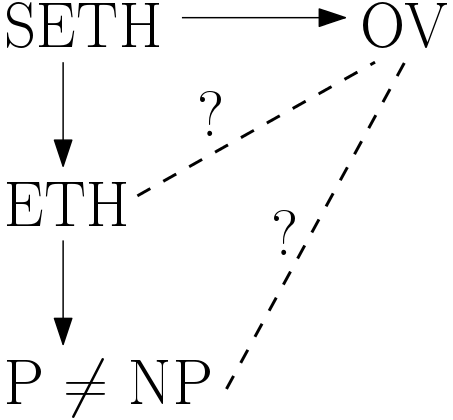
\includegraphics[scale=0.6]{sethOVDiag.png}
%	\caption{The relationships between SETH (strong exponential time hypothesis), ETH (exponential time hypothesis), OV (orthogonal vectors) and P vs NP. The dotted lines signify that we don't know the relationship}
%	\label{fig:sethOVRelationship}
%\end{figure}


%\subsection{Previous Works}
%There has been much prior work leading up to our results. First, there are a few results using assumptions from fine-grained complexity and applying them to cryptography. Second, there has been work with the kind of assumptions that we will be using. 
%
%%TODO: The organization of this section needs work...
%%TODO: merkle puzzles first as weak crypto?
%%TODO: talk about Ball et al stuff first as they try to answer this question, then Vinod's paper, Subset Sum -> k-Sum etc (similar assumptions), and SS -> PKC
%
%
%\subsubsection{Fine-Grained Cryptography}
%Ball et al. \cite{avgCaseFineGrained,eprintAvgCaseFG} considered the key hard problems from fine-grained complexity and showed that one can obtain problems that are hard on average, in a fine-grained sense, using fine-grained worst case to average case reductions. They established useful definitions of fine-grained one-way functions, and derived the first proof-of-work in the fine-grained setting, based on a {\em worst-case} assumption from fine-grained complexity. However, their approach was not sufficient to give a construction of one-way-functions (or public-key cryptography), and indeed Ball et al. proved a limitation of their approach in this regard - extending their approach would falsify the Nondeterministic Strong Exponential Time Hypothesis of Carmosino et al. \cite{CarmosinoGIMPS16}. Because of this seeming barrier, one would either need to develop brand new techniques, or use a different hardness assumption.
%
%
%%These notions are similar to ours in that they make stronger assumptions on the power of an adversary, but while they rely on circuit complexity, which allows them to make unconditional statements, we rely on the more general computational complexity of problems.
%
%
%\paragraph{Fine-Grained Key Exchanges.} Fine-grained cryptography is a relatively unexplored area, even though it had its start in the 1970's with Merkle puzzles: the gap between honestly participating in the protocol versus breaking the security guarantee was only quadratic \cite{Merkle78}. Merkle originally did not describe a plausible hardness assumption under which the security of the key exchange can be based. 30 years later, Biham, Goren, and Ishai showed how to implement Merkle puzzles by making an assumption of the existence of either a random oracle or an exponential gap one way function \cite{BGI08}. That is, Merkle puzzles were built under the assumption that a one-way function exists which takes time $2^{n(1/2+\delta)}$ to invert for some $\delta>0$. So while prior work indeed succeeded in building a fine-grained key-exchange, it need for a very strong variant of OWFs to exist. It is thus very interesting in particular to obtained fine-grained public key encryption schemes based on a fine-grained assumption (and hence might even work in Pessiland and below).
%
%\paragraph{Another notion of Fine-Grained Cryptography.} In 2016, work by Degwekar, Vaikuntanathan, and Vasudevan \cite{DVV16} discussed fine-grained complexity with respect to both honest parties and adversaries restricted to certain circuit classes. They obtained constructions for some cryptographic primitives (including PKE) when restricting an adversary to a certain circuit class. From the assumption $\mathsf{NC}1 \neq \xor L/\poly$ they show Alice and Bob can be in $AC^0[2]$ while being secure against $\mathsf{NC}1$ adversaries. While \cite{DVV16} has some unconditional constructions, their security relies on the circuit complexity of the adversary, and does not apply to arbitrary time-bounded adversaries as is usually the case in cryptography. That is, this restricts the types of algorithms an adversary is allowed to use beyond just how much runtime these algorithms can have. It would be interesting to get similar results in the low-polynomial time regime, without circuit complexity assumptions.
%
%
%
%\begin{figure}
	%\begin{center}
		%\begin{tabular}{| l | l | l | l | l |}
			%\hline
			%Paper & Assumptions & Crypto & Runtime & \begin{tabular}{l} Power of\\ Adversary
			%\end{tabular} \\\hline
			%\cite{Merkle78} & Random Oracles* & Key Exchange & $O(N)$ & $O(N^2)$\\\hline
			%\cite{BGI08} & Exponentially-Strong OWFs & Key Exchange & $O(N)$ & $O(N^2)$ \\\hline
			%\cite{eprintAvgCaseFG} & WC 3-sum, OV, APSP, or SETH & Proof of Work & $O(N^2)$ & N/A \\\hline
			%[This work] & \zkclique~or $k$-sum & \begin{tabular}{l} OWFs,\\
				%Key Exchange \& PKE
			%\end{tabular} &\begin{tabular}{l}
			%$O(N)$\\
			%$O(N)$
		%\end{tabular} & \begin{tabular}{l}
		%$O(N^{1 + \delta})$\\
		%$O(N^{1.5 - \delta})$
	%\end{tabular} \\\hline
	%\cite{DVV16} & $\mathsf{NC}1 \neq \xor L/\poly$ & \begin{tabular}{l}
		%OWFs, and PRGs\\
		%with sublinear \\
		%stretch, CRHFs, \\
		%and PKE\\ \\
	%\end{tabular} &$\mathsf{NC}1$ &$\mathsf{NC}1$\\
	%&$\mathsf{NC}1 \neq \xor L/\poly$ &\begin{tabular}{l} PKE and CRHFs\\ \\
	%\end{tabular}  & $\mathsf{AC}^0[2]$&$\mathsf{NC}1$ \\
	%& Unconditional &\begin{tabular}{l}
		%PRGs with poly\\
		%stretch, Symmetric\\
		%encryption,\\
		%and CRHFs\\
	%\end{tabular}  & $\mathsf{AC}^{0}$ & $\mathsf{AC}^0$\\\hline
%\end{tabular}
%\caption{\label{fig:comparison} A table of previous works' results in this area. There have been several results characterizing different aspects of fine-grained cryptography. *It was \cite{BGI08} who showed that Merkle's construction could be realized with a random oracle. However, Merkle presented the construction.  }
%\end{center}
%\end{figure}
%
%
%
%\subsubsection{Similar Assumptions}
%This paper uses many assumptions that, while solvable in polynomial time, are variants of natural NP-hard problems, in which the size of the solution is a fixed constant. For instance, for constant $k$, $k$-SUM is the variant of Subset Sum, where we are given $n$ numbers and we need to find exactly $k$ elements that sum to a given target, and Zero-$k$-Clique is the variant of Zero-Clique, in which we are given a graph and we need to find exactly  $k$ nodes that form a clique whose edge weights sum to zero.
%
%With respect to Subset Sum, Impagliazzo and Naor showed how to directly obtain OWFs and PRGs assuming that Subset Sum is hard on average \cite{IN02}. The OWF is $f(\vec a, \vec s) = \vec a \cdot \vec s$, where $\vec a$ is the list of elements (chosen uniformly at random from the range $R$) and $s \in \{0,1\}^n$ represents the set of elements we add together.
%In addition to Subset Sum, OWFs have also been constructed from planted Clique, SAT, and Learning-Parity with Noise \cite{Lindell,JP00}. The constructions from \cite{Lindell} come from a definition of a ``plantable'' NP-hard problem that is assumed to be hard on average.
%
%%Although our OWFs are essentially equivalent to scaled-down, polynomial-time solveable characterizations of these problems, we also formalize the property that allows us to get these fine-grained OWFs (plantability). We combine these NP constructions and formalizations to lay the groundwork for fine-grained cryptography.
%
%In more recent work, Subset Sum was also shown to directly imply public-key cryptography \cite{LPS10}. The construction takes ideas from Regev's LWE construction, turning a vector of subset sum elements into a matrix by writing each element out base $q$ in a column. The subset is still represented by a 0-1 matrix, and error is handled by the lack of carrying digits. It is not clear how to directly translate this construction into the fine-grained world, and even less clear what the benefit would be; directly converting from Subset Sum to $k$-Sum just significantly weakens the security without added benefit. A very desirable goal is to obtain novel cryptographic approaches exploiting the fine-grained nature of these problems, going beyond just recasting normal cryptography in the fine-grained world.
%
%

%%%%%%%%%%%%%%%%%%%new work%%%%%%%%%%%%%

\subsection{Our contributions}
%***NEEDS to CHANGE***
%Our main result is a weak key-exchange from a merely polynomial time fine-grained assumption, exploring cryptographic protocols that may maintain security even if $P=NP$. We also obtain a fine-grained version of hardcore bits.

Our main result is a fine-grained key-exchange that can be formed from any problem that meets three structural conditions in the word-RAM model of computation. This addresses the question of what properties are sufficient to produce fine-grained Public Key Encryption schemes (PKEs).
%We show that three properties we define are sufficient to build a fine-grained PKE.


%We describe the assumptions we use and then describe our public key exchange. 
%Then, we explore fine-grained OWFs, showing that hardcore bits, and other basic functionality are not immediate in the fine-grained cryptography world, and also providing a notion of fine-grained hardcore bits that we can achieve. 

For our key exchange, we describe a set of properties, and any problem that has those properties implies a polynomial gap PKE. An informal statement of our main theorem is as follows.\\


\begin{theoremNon}[Fine-Grained Key-Exchange (informal)]
Let $P$ be a computational problem for which a random instance can be generated in $O(n^g)$ time for some $g$, and that
requires $n^{k-o(1)}$ time to be solved on average for some fixed $k>g$.
Additionally, let $P$ have three key structural properties of interest: (1) ``plantable'': we can generate a random-looking instance, choosing either to have or not to have a solution in the instance, and if there is a solution, we know what/where it is; (2)
``average-case list-hard'':  
given a list of $n$ random instances
of the problem, returning which one of the instances has a solution requires essentially
solving all instances;
(3) ``splittable'': when given an instance with a solution, we can
split it in $O(n^g)$ time into two slightly smaller instances that both have solutions.

Then a public key-exchange can be built such that Alice and Bob exchange a $\lg(n)$ bit key in time $n^{2k-g}$, where as Eve must take $\tilde{\Omega}(n^{3k-2g})$ time to learn Alice and Bob's key.
\end{theoremNon}\\

Notice that as long as there is a gap between the time to generate a random instance and the time to solve an instance on average, there is a gap between $N=n^{2k-g}$ and $n^{3k-2g}=N^{3/2 - 1/(4(k/g)-2)}$ and the latter goes to $N^{3/2}$, as $k/g$ grows.
The key exchange requires no interaction, and we get a \emph{fine-grained} public key cryptosystem.
While our key exchange construction provides a relatively small gap between the adversary and the honest parties ($O(N^{1.5})$ vs $O(N)$),  the techniques required to prove security of this scheme are novel and the result is generic as long as the three assumptions are satisfied. In fact, we will show an alternate method to achieve a gap approaching $O(N^2)$ in the full version of this paper.


Our main result above is stated formally and in more generality in Theorem \ref{thm:fg-pkc}. We will explain the formal meaning of our structural properties  \emph{plantable}, \emph{average-case list-hard}, and \emph{splittable} later. 

%(3k-2g)/(2k-g) = *3/2*(2k-g) -0.5g)

We also investigate what plausible average-case assumptions one might be able to make about the key problems from fine-grained complexity so that the three properties from our theorem would be satisfied.
We consider the \zkclique~problem as it is one of the hardest worst-case problems in fine-grained complexity. For instance, it is known that if \zThclique~is in $O(n^{3-\eps})$ time for some $\eps>0$, then both the \ThSum~and the APSP hypotheses are violated \cite{icm-survey,WilliamsW13j}. It is important to note that while fine-grained problems like \zkclique~and \kSum~are suspected to take a certain amount of time in the worst case, when making these assumptions for any constant $k$ does not seem to imply $P \neq NP$ since all of these problems are still solveable in polynomial time.\footnote{Assuming the hardness of these problems for more general $k$ will imply $P \neq NP$, but that is not the focus of our work.}

An instance of \zkclique~is a complete $k$-partite graph $G$, where each edge is given a weight in the range $[0,R-1]$ for some integer $R$. The problem asks whether there is a $k$-clique in $G$ whose edge weights sum to $0$, modulo $R$. A standard fine-grained assumption (see e.g. \cite{icm-survey}) is that in the worst case, for large enough $R$, say $R\geq 10n^{4k}$, \zkclique~requires $n^{k-o(1)}$ time to solve. 
\zkclique~has no non-trivial average-case algorithms for natural distributions (uniform for a range of parameters, similar to \kSum~and Subset Sum). Thus, \zkclique~is a natural candidate for an average-case fine-grained hard problem.
\\

%\begin{theoremNon}[Fine-Grained Key-Exchange (intuitive)]
%	If the zero-$k$-Clique problem is $n^{k-o(1)}$ hard on average then a public key-exchange can be built such that Alice and Bob exchange a $\lg(n)$ bit key in time $n^{2k-2}$, whereas Eve must take $\tilde{\Omega}(n^{3k-4})$ time to learn Alice and Bob's key. 
%\end{theoremNon}
%\\



%Our contribution to this line of work is the first fine-grained key exchange based on a fine-grained combinatorial assumption (see Section \ref{sec:averageCaseAssumptions} for details on our assumption). 

%Because our construction provides a non-interactive key exchange, we also build a public-key cryptosystem out of assumptions that are both combinatorial and related to the assumptions used for one-way functions, as opposed to those used for trap-door functions.

Our other contribution addresses an open question from Ball et al.: can a fine-grained one-way function be constructed from worst case assumptions? While we do not fully achieve this, we generate new plausible average-case assumptions from fine-grained problems that imply fine-grained one-way functions. %We also explore how these fine-grained OWFs can generate fine-grained hardcore bits. The standard Goldreich-Levin construction \cite{hardCoreBitsAndXorLemmaFromGL} does not directly work, so we devise a natural variant of fine-grained hardcore bits and develop methods to generate them.


\subsection{Previous Works}
There has been much prior work leading up to our results. First, there are a few results using assumptions from fine-grained complexity and applying them to cryptography. Second, there has been work with the kind of assumptions that we will be using. 

%TODO: The organization of this section needs work...
%TODO: merkle puzzles first as weak crypto?
%TODO: talk about Ball et al stuff first as they try to answer this question, then Vinod's paper, Subset Sum -> k-Sum etc (similar assumptions), and SS -> PKC


\subsubsection{Fine-Grained Cryptography}
Ball et al. \cite{avgCaseFineGrained,eprintAvgCaseFG} produce fine-grained wost-case to average-case reductions. Ball et al. leave an open problem of producing a one-way-function from a worst case assumption. They prove that from some fine-grained assumptions building a one-way-function would falsify NSETH \cite{CarmosinoGIMPS16}\cite{avgCaseFineGrained}.
%Ball et al. \cite{avgCaseFineGrained,eprintAvgCaseFG} considered the key hard problems from fine-grained complexity and showed that one can obtain problems that are hard on average, in a fine-grained sense, using fine-grained worst-case to average-case reductions. They established useful definitions of fine-grained one-way functions, and derived the first proof-of-work in the fine-grained setting, based on a {\em worst-case} assumption from fine-grained complexity. However, their approach was not sufficient to give a construction of one-way-functions (or public-key cryptography), and indeed Ball et al. proved a limitation of their approach in this regard - extending their approach would falsify the Nondeterministic Strong Exponential Time Hypothesis of Carmosino et al. \cite{CarmosinoGIMPS16}. Because of this seeming barrier, one would either need to develop brand new techniques, or use a different hardness assumption.
We avoid their barrier in this paper by producing a construction of both fine-grained OWFs and fine-grained PKE from an \emph{average-case} assumption.
%We choose to do the latter in this paper, producing a construction of both fine-grained OWFs and fine-grained PKE from an \emph{average-case} assumption. So, the question of how to build OWFs from worst case fine-grained complexity assumptions that was left open by Ball et al. is still open. However, our demonstration of explicit constructions for a fine-grained PKE from polynomial problems begins to classify what polynomial time assumptions result in public key cryptography. %opens the possibility of cryptography when no strong OWFs exist. 


%However, Merkel puzzle constructions require a OWF that is not invertible in $2^{n(\frac{1}{2}+\epsilon)}$ time for some $\epsilon>0$. So while this is a fine-grained exponential assumption, we only require a fine-grained polynomial assumption.




\paragraph{Fine-Grained Key Exchanges.} Fine-grained cryptography is a relatively unexplored area, even though it had its start in the 1970's with Merkle puzzles: the gap between honestly participating in the protocol versus breaking the security guarantee was only quadratic \cite{Merkle78}. Merkle originally did not describe a plausible hardness assumption under which the security of the key exchange can be based. 30 years later, Biham, Goren, and Ishai showed how to implement Merkle puzzles by making an assumption of the existence of either a random oracle or an exponential gap one way function \cite{BGI08}. That is, Merkle puzzles were built under the assumption that a one-way function exists which takes time $2^{n(1/2+\delta)}$ to invert for some $\delta>0$. So while prior work indeed succeeded in building a fine-grained key-exchange, it needed a very strong variant of OWFs to exist. It is thus very interesting to obtain fine-grained public key encryption schemes based on a fine-grained assumption (that might even work in Pessiland and below).

%Considering Merkle Puzzles and other cryptographic assumptions, one may be concerned that a fine-grained assumption is as strong as, say, assuming that exponentially-hard OWFs exist. However, these two assumptions are essentially orthogonal to each other, and in some senses standard cryptographic assumptions are stronger. For example, the standard notion of OWFs trivially imply that fine-grained OWFs exist, but there is no known way of showing the reverse.

% Merkel Puzzles
%The known constructions of Merkle puzzles produce fine-grained PKE from fine-grained exponential OWFs \cite{Merkle78,BGI08,optimalMerklePuzzles}. We are able to build a only slightly weaker PKE from a \textit{polynomial} time hardness assumption. Furthermore, we show that a class of  polynomial time fine-grained assumptions lead to fine-grained PKEs.%As we mentioned earlier, our assumption might still hold even if exponential OWFs do not exist.
%TODO: make sure this meshes with the above

\paragraph{Another notion of Fine-Grained Cryptography.} In 2016, work by Degwekar, Vaikuntanathan, and Vasudevan \cite{DVV16} discussed fine-grained complexity with respect to both honest parties and adversaries restricted to certain circuit classes. They obtained constructions for some cryptographic primitives (including PKE) when restricting an adversary to a certain circuit class. From the assumption $\mathsf{NC}1 \neq \xor L/\poly$ they show Alice and Bob can be in $AC^0[2]$ while being secure against $\mathsf{NC}1$ adversaries. While \cite{DVV16} obtains some unconditional constructions, their security relies on the circuit complexity of the adversary, and does not apply to arbitrary time-bounded adversaries as is usually the case in cryptography. That is, this restricts the types of algorithms an adversary is allowed to use beyond just how much runtime these algorithms can have. It would be interesting to get similar results in the low-polynomial time regime, without restricting an adversary to a certain circuit class. Our results achieve this, though not unconditionally.

\paragraph{Tight Security Reductions and Fine-Grained Crypto.}
Another area the world of fine-grained cryptography collides with is that of tight security reductions in cryptography. Bellare et.al. coined the term ``concrete'' security reductions in \cite{BellareKR94,BellareGR95}. Concrete security reductions are parametrized by time ($t$), queries ($q$), size ($s$), and success probability ($\eps$). 
%This definition stated that a program (adversary) could only run in time $t$, making $q$ queries of size at most $\ell$, to some oracle for a function, can only succeed with probability at most $\epsilon$ in solving some problem.
This line of work tracks how a reduction from a problem to a  construction of some cryptographic primitive effects the four parameters of interest.  
%This line of work relies on seeing how exactly a reduction from a problem that is $(t,q,\ell,\epsilon)$-secure to a construction of some cryptographic primitive is comparably secure, keeping track of how $t$, $q$, $\ell$, and $\epsilon$ change. 
This started a rich field of study connecting theory to practical cryptographic primitives (such as PRFs, different instantiations of symmetric encryption, and even IBE for example \cite{BellareCK96,BellareDJR97,KatzW03,BellareR09}). %Since we are not guaranteed much in terms of security or even a negligible advantage in our fine-grained setting, 
In fine-grained reductions we also need to track exactly how our adversary's advantage changes throughout our reductions, however, we also track the running time of the honest parties. % --- at least up to the nearest polynomial. However, we also seek to convey the security in our constructions in a way that makes it relatively easy to compose schemes without needing to worry too much about runtime. 
So, unlike in the concrete security literature, when the hard problems are polynomially hard (perhaps because $P=NP$), we can track the gap in running times between the honest and dishonest parties. This allows us to build one way functions and public key cryptosystems when the hard problems we are given are only polynomially hard. 
%So, unlike in the concrete security literature, we ignore log factors and instead focus on $\~O$ notation.
%%%TODO: this is not a convincing differece between their work and ours

\vspace{-0.5cm}

\begin{figure}
	\begin{center}
		\begin{tabular}{| l | l | l | l | l |}
			\hline
			Paper & Assumptions & Crypto & Runtime & \begin{tabular}{l} Power of\\ Adversary
			\end{tabular} \\\hline
			\cite{Merkle78} & Random Oracles* & Key Exchange & $O(N)$ & $O(N^2)$\\\hline
			\cite{BGI08} & Exponentially-Strong OWFs & Key Exchange & $O(N)$ & $O(N^2)$ \\\hline
			\cite{eprintAvgCaseFG} & WC \ThSum, OV, APSP, or SETH & Proof of Work & $O(N^2)$ & N/A \\\hline
			[This work] & \zkclique~or \kSum& \begin{tabular}{l} OWFs,\\
				Key Exch. \& PKE
			\end{tabular} &\begin{tabular}{l}
			$O(N)$\\
			$O(N)$
		\end{tabular} & \begin{tabular}{l}
		$O(N^{1 + \delta})$\\
		$O(N^{1.5 - \delta})$
	\end{tabular} \\\hline
	\cite{DVV16} & $\mathsf{NC}1 \neq \xor L/\poly$ & \begin{tabular}{l}
		OWFs, and PRGs\\
		with sublinear \\
		stretch, CRHFs, \\
		and PKE\\ \\
	\end{tabular} &$\mathsf{NC}1$ &$\mathsf{NC}1$\\
	&$\mathsf{NC}1 \neq \xor L/\poly$ &\begin{tabular}{l} PKE and CRHFs\\ \\
	\end{tabular}  & $\mathsf{AC}^0[2]$&$\mathsf{NC}1$ \\
	& Unconditional &\begin{tabular}{l}
		PRGs with poly\\
		stretch, Symmetric\\
		encryption,\\
		and CRHFs\\
	\end{tabular}  & $\mathsf{AC}^{0}$ & $\mathsf{AC}^0$\\\hline
\end{tabular}
\caption{\label{fig:comparison} A table of previous works' results in this area. There have been several results characterizing different aspects of fine-grained cryptography. *It was \cite{BGI08} who showed that Merkle's construction could be realized with a random oracle. However, Merkle presented the construction.  }
\end{center}
\end{figure}
%\vspace{-1.22cm}
\subsubsection{Similar Assumptions}
This paper uses hypotheses on the running times of problems that, while solvable in polynomial time, are variants of natural NP-hard problems, in which the size of the solution is a fixed constant. For instance, \kSum~is the variant of Subset Sum, where we are given $n$ numbers and we need to find exactly $k$ elements that sum to a given target, and \zkclique~is the variant of Zero-Clique, in which we are given a graph and we need to find exactly $k$ nodes that form a clique whose edge weights sum to zero.

With respect to Subset Sum, Impagliazzo and Naor showed how to directly obtain OWFs and PRGs assuming that Subset Sum is hard on average \cite{IN02}. The OWF is $f(\vec a, \vec s) = (\vec a, \vec a \cdot \vec s)$, where $\vec a$ is the list of elements (chosen uniformly at random from the range $R$) and $s \in \{0,1\}^n$ represents the set of elements we add together.
In addition to Subset Sum, OWFs have also been constructed from planted Clique, SAT, and Learning-Parity with Noise \cite{Lindell,JP00}. The constructions from the book of Lindell and the chapter written by Barak \cite{Lindell} come from a definition of a ``plantable'' NP-hard problem that is assumed to be hard on average.

Although our OWFs are equivalent to scaled-down, polynomial-time solvable characterizations of these problems, we also formalize the property that allows us to get these fine-grained OWFs (plantability). We combine these NP constructions and formalizations to lay the groundwork for fine-grained cryptography.

In the public-key setting, there has been relatively recent work taking NP-hard problems and directly constructing public-key cryptosystems \cite{ABW10}. They take a problem that is NP-hard in its worst case and come up with an average-case assumption that works well for their constructions. Our approach is similar, and we also provide evidence for why our assumptions are correct.

In recent work, Subset Sum was also shown to directly imply public-key cryptography \cite{LPS10}. The construction takes ideas from Regev's LWE construction \cite{Regev05}, turning a vector of subset sum elements into a matrix by writing each element out base $q$ in a column. The subset is still represented by a 0-1 matrix, and error is handled by the lack of carrying digits. It is not clear how to directly translate this construction into the fine-grained world. First, directly converting from Subset Sum to \kSum~just significantly weakens the security without added benefit. More importantly, the security reduction has significant polynomial overhead, and would not apply in a very pessimistic Pessiland where random planted Subset Sum instances can be solved in quadratic time, say.

While it would be interesting to reanalyze the time-complexity of this construction (and others) in a fine-grained way, this is not the focus of our work. Our goal is to obtain novel cryptographic approaches exploiting the fine-grained nature of the problems, going beyond just recasting normal cryptography in the fine-grained world, and obtaining somewhat generic constructions.


\subsection{Technical Overview}
Here we will go into a bit more technical detail in describing our results. First, we need to describe our hardness assumptions. Then, we will show how to use them for our fine-grained key exchange, and finally, we will talk briefly about fine-grained OWFs and hardcore bits.

\paragraph{Our Hardness Assumption} %TODO: Be precise about modulus etc

We generate a series of properties where if a problem has these properties then a fine-grained public key-exchange can be built.

One property we require is that the problem is hard on average, in a fine-grained sense. Intuitively, a problem is average case indistinguishably hard if given an instance that is drawn with probability $1/2$ from instances with no solutions and with probability $1/2$ from instances with one solution, it is computationally hard on average to distinguish whether the instance has $0$ or $1$ solutions.
The rest of the properties are structural; we need a problem that is \emph{plantable}, \emph{average-case list-hard}, and \emph{splittable}. Informally,

\begin{itemize}
	\item The plantable property roughly says that one can efficiently choose to generate either an instance without a solution or one with a solution, knowing where the solution is; %A problem is plantable if, we can generate a random-looking instance, choosing either to have or not to have a solution in the instance, and if there is a solution, we know what/where it is;
	%when given a random instance without a solution, we can \emph{plant} one, and have the resulting output ``look'' random;
	\item The average case list-hard property says that if one is given a list of instances where all but one of them are drawn uniformly over instances with no solutions, and a random one of them is actually drawn uniformly from instances with one solution, then it is computationally hard to find the instance with a solution;
	\item Finally, the splittable property says that one can generate from one average case instance, two new average case instances that have the same number of solutions as the original one. %A problem is splittable if when given an instance with a solution, we can split it into two slightly smaller instances that \emph{both} have solutions.
\end{itemize}
These are natural properties for problems and hypotheses to have. We will demonstrate in Section \ref{sec:zkcIsAllTheThings} that \zkclique~has all of these properties. We need our problem to have all three of these qualities for the key exchange. For our one-way function constructions we only need the problem to be plantable.

%The strong version of our \zkclique~assumption satisfies all of three of these properties. %For the remainder of this overview, we will be using the assumption that we can generate a planted \zkclique~instance in time $O(n^2)$ and it takes $O(n^k)$ for any randomized adversary to find the clique. In section \ref{sec:fg-owfs}, we show that we can relax this assumption for constructing both key exchanges and fine-grained OWFs.

%Usefully, our properties also immediately imply the existence of a fine-grained one-way function based on the problem that satisfies them.

The structural properties are quite generic, and in principle, there could be many problems that satisfy them. We exhibit one: the \zkclique~problem.

Because no known algorithmic techniques seem to solve \zkclique~even when the weights are selected independently uniformly at random from $[0,cn^k]$ for a constant $c$, folklore intuition dictates that the problem might be hard on average for this distribution: here, the expected number of $k$-Cliques is $\Theta(1)$, and solving the decision problem correctly on a large enough fraction of the random instances seems difficult.
This intuition was formally proposed by Pettie~\cite{avgCase3Sum} for the very related \kSum~problem which we also consider.

We show that the \zkclique~problem, together with the assumption that it is fine-grained hard to solve on average, satisfies all of our structural properties, and thus, using our main theorem, one can obtain a fine-grained key exchange based on 
\zkclique.

\textit{Key Exchange Assumption.} We assume that when given a complete $k$-partite graph with $kn$ nodes and random weights $[0,R-1]$, $R = \Omega(n^k)$, any adversary running in time $n^{k-\Omega(1)}$ time cannot distinguish an instance with a zero-$k$-clique solution from one without with more than $2/3$ chance of success.
In more detail, consider a distribution where with probability $1/2$ one generates a random instance of size $n$ with no solutions, and with probability $1/2$ one generates a random instance of size $n$ with exactly one solution. (We later tie in this distribution to our original uniform distribution.) Then, consider an algorithm that can determine with probability $2/3$ (over the distribution of instances) whether the problem has a solution or not.
%We first hypothesize that any such algorithm for \kSum~or \zkclique~must take super-linear time. From this weak assumption we can get one-way functions. 
We make the conjecture that such a $2/3$-probability distinguishing algorithm for \zkclique, which can also exhibit the unique zero clique whenever a solution exists, 
requires time $n^{k-o(1)}$.



\paragraph{Public Key Exchange}

So, what does the existence of a problem with our three properties, \emph{plantable}, \emph{average-case list-hard}, and \emph{splittable}, imply?

The intuitive statement of our main theorem is that, if a problem has the three properties, and is $n^k$ hard to solve on average and can be generated in $n^g$ time (for \zkclique~$g=2$), then a key exchange exists that takes $O(N)$ time for Alice and Bob to execute, and requires an eavesdropper Eve $\tilde{\Omega}(N^{(3k-2g)/(2k-g)})$ time to break. When $k>g$ Eve takes super linear time in terms of $N$. When $k=3$ and $g=2$, an important case for the \zkclique~problem, Eve requires $\tilde{\Omega}(N^{5/4})$ time. 

For the rest of this overview we will describe our construction with the problem \zkclique. 

To describe how we get our key exchange, it is first helpful to consider Merkle Puzzles \cite{Merkle78,BGI08,optimalMerklePuzzles}. The idea is simple: let $f$ be a one way permutation over $n$ bits (so a range of $2^n$ values) requires $2^{n(\frac{1}{2}+\epsilon)}$ time to invert for some constant $\epsilon>0$. Then, Alice and Bob could exchange a key by each computing $f(v)$ on  $10\cdot2^{n/2}$ random element $v \in [2^{n}]$ and sending those values $f(v)$ to each other. With .9 probability, Alice and Bob would agree on at least one pre-image, $v$. It would take an eavesdropper Eve $\Omega(2^{n(\frac{1}{2}+\epsilon)})$ time before she would be able to find the $v$ agreed upon by Alice and Bob. So, while Alice and Bob must take $O(2^{n/2})$ time, Eve must take $O(2^{n(\frac{1}{2}+\epsilon)})$ time to break it. 

%Specifically, assume there exists a one way function, $f$, over $\{0,1\}^n$ that can be computed in polynomial time, but requires $2^{n(\frac{1}{2}+\epsilon)}$ time to invert. Then, using Merkle Puzzles, the two honest parties, Alice and Bob could do $N=\Theta^*(2^{n/2})$ work to exchange an index of size $\lg(N)=n$. If an eavesdropper Eve wanted to also learn the key, she would need to put in $N^{1+2\epsilon}=\Omega^*(2^{n(\frac{1}{2}+\epsilon)})$ work. 

%\emph{fine-grained} exponential assumption. The assumption is simultaneously exponential and sensitive to multiplicative constants. Notably, a one way permutation that requires $2^{n\frac{1}{3}}$ time to invert does not imply the existence of a fine-grained key-exchange via this strategy. 

Our construction will take on a similar form: Alice and Bob will send several problems to each other, and some of them will have planted solutions. By matching up where they both put solutions, they get a key exchange.

Concretely, Alice and Bob will exchange $m$ instances of the \zkclique~problem and in $\sqrt{m}$ of them (chosen at random), plant solutions. The other $m - \sqrt{m}$ will not have solutions (except with some small probability). These $m$ problems will be indexed, and we expect Alice and Bob to have both planted a solution in the same index. Alice can check her $\sqrt{m}$ indices against Bob's, while Bob checks his, and by the end, with constant probability, they will agree on a single index as a key. In the end, Alice and Bob require $O(mn^g + \sqrt{m}n^{k})$ time to exchange this index.  Eve must take time $\tilde{\Omega}(n^{k}m)$. When  $m = n^{2k-2g}$, Alice and Bob take $O(n^{2k-g})$ time and Eve takes $\tilde{\Omega}(n^{3k-2g})$. We therefore get some gap between the running time of Alice and Bob as compared to Eve for any value of $k\geq g$. Furthermore, for all $\delta>0$ there exists some large enough $k$ such that the difference in running time is at least $O(T(n))$ time for Alice and Bob and $\tilde{\Omega}(T(n)^{1.5-\delta})$ time for Eve. Theorem \ref{thm:fg-pkc} is the formal theorem statement.



\begin{figure}[h]
	\centering
	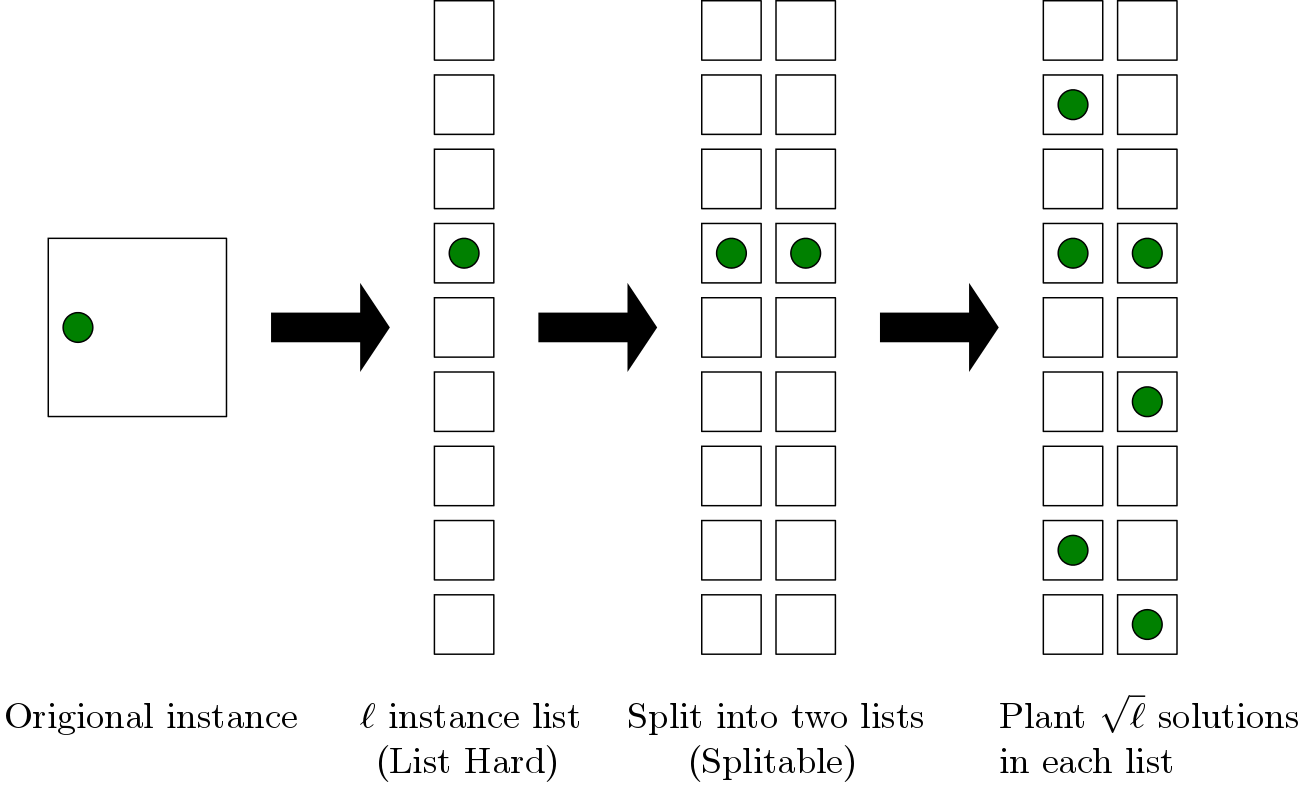
\includegraphics[scale=0.6]{fgcrypto/FullReduction.png}
	\caption{A depiction of our reduction showing hardness for our fine-grained key exchange.}
	\label{fig:wholeReductionBoxes}
\end{figure}

To show hardness for this construction we combine techniques from both fine-grained complexity and cryptography (see Figure \ref{fig:wholeReductionBoxes}). We take a single instance and use a self-reduction to produce a list of $\ell$ instances where one has a solution whp if the original instance has a solution. In our reductions $\ell$ will be polynomial in the input size. Then, we take this list and produce two lists that have a solution in the same location with high probability if the original instance has a solution. Finally, we plant $\sqrt{\ell}$ solutions into the list, to simulate Alice and Bob's random solution planting. 

%\xxx{Rio: Need to put a theorem statement in here}
%\begin{theorem}[Fine-Grained Key-Exchange (informal)]
%Let $P$ be an average case problem that can be generated and planted in time $n^2$, but requires $n^{k-o(1)}$ to be solved where $k>2$. Additionally, let $P$ be \emph{plantable}, \emph{average-case list-hard}, and \emph{splittable}.

%Then a public key-exchange can be built such that Alice and Bob exchange a $\lg(n)$ bit key in time $n^{2k-2}$, where as Eve must take $\tilde{\Omega}(n^{3k-4})$ time to learn Alice and Bob's key. 
%\end{theorem}


%We present a set of three general properties where if a problem has those properties then a fine-grained key exchange exists. These properties are that the problem must be \emph{plantable}, \emph{average }


\paragraph{One Way Functions}
%\xxx{Rio: Need to rewrite to put in context of other OWF definitions. Also note the Yao part.}
First, and informally, a fine-grained OWF is a function on $n$ bits that requires $\~O(T(n)^{1-\delta})$ time to evaluate for some constant $\delta > 0$, and if any adversary attempts to invert $f$ in time $\~O(T(n)^{1 - \delta'})$ for \emph{any} constant $\delta' > 0$, she only succeeds with probability at most $\epsilon(n)$, where $\epsilon$ is considered ``insignificant.''

Ball et al. \cite{avgCaseFineGrained} defined fine-grained OWFs, keeping track of the time required to invert and the probability of inversion in two separate parameters. We streamline this definition by fixing the probability an adversary inverts too an insignificant function of input size, which we define in Section \ref{sec:prelims}. %It will turn out that this notion of insignificance will extend to our definition of hardcore bits.

For this overview, we will focus on the intuition of using specific problems \kSum-$R$ (\kSum~modulo $R$) or \zkclique-$R$ (\zkclique~modulo $R$) to get fine-grained OWFs, though in section \ref{sec:fg-owfs}, we construct fine-grained OWFs from a general class of problems. Let $N$ be the size of the input to these problems. Note that if $R$ is too small (e.g. constant), then these problems are solvable quickly and the assumptions we are using are false. So, we will assume $R = \Omega(n^k)$.

\textit{OWF Assumptions.} Much like for our key exchange, our assumptions are about the difficulty of distinguishing an instance of \kSum~or \zkclique~with probability more than $2/3$ in time faster than $n^{k/2}$ or $n^k$ respectively. Formally, randomly generating a \kSum-$R$ instance is creating a $k$ lists of size $n$ with values randomly chosen from $[0,R-1]$. Recall that a random \zkclique~instance is a complete $k$-partite graph where weights are randomly chosen from $[0,R-1]$. Our `weak' \kSum-$R$ and \zkclique-$R$ assumptions state that for any algorithm running in $O(n)$ time, it cannot distinguish between a randomly generated instance with a planted solution and one without with probability greater than $2/3$.

Note that these assumptions are much weaker than the previously described key-exchange assumption, where we allowed the adversary $O(n^{k-\Omega(1)})$ time instead of just super-linear.

\begin{theorem}[Fine-Grained OWFs (informal)]
	If for some constant $\delta>0$ and range $R = \Omega(n^k)$ either \kSum-$R$ requires $\Omega(N^{1+\delta})$ time to solve with probability $>2/3$ or \zkclique-$R$ requires $\Omega(N^{(1+\delta)})$ time to solve with probability $>2/3$  then a fine-grained OWF exists.
\end{theorem}
The formal theorem is Theorem \ref{thm:FGOWFs-exist} and is proved in Appendix \ref{sec:building-fgowfs}.

Intuitively our construction of a fine-grained OWF runs a planting procedure on a random instance in time $O(N)$. By our assumptions finding this solution takes time $\Omega(N^{1+\delta})$ for some constant $\delta > 0$, and thus inverting this OWF takes $\Omega(N^{1+\delta})$.

We also get a notion of hardcore bits from this. Unlike in traditional crypto, we can't immediately use Goldreich-Levin's hardcore bit construction \cite{hardCoreBitsAndXorLemmaFromGL}. Given a function on $N$ bits, the construction requires at least $\Omega(N)$ calls to the adversary who claims to invert the hardcore bit. When one is seeking super-polynomial gaps between computation and inversion of a function, factors of $N$ can be ignored. However, in the fine-grained setting, factors of $N$ can completely eliminate the gap between computation and inversion, and so having a notion of fine-grained hardcore bits is interesting.

We show that for our concrete constructions of fine-grained OWFs, there is a subset of the input of size $O(\lg(N))$ (or any sub-polynomial function) which itself requires $\Omega(N^{1+\delta})$ time to invert. From this subset of bits we can use Goldreich-Levin's hardcore bit construction, only losing a factor of $N^{o(1)}$ which is acceptable in the fine-grained setting.

\begin{theorem}[Hardcore Bits (informal)]
	If for some constant $\delta>0$ and range $R = \Omega(n^k)$ either \kSum-$R$ requires $\Omega(N^{1+\delta})$ time to solve with probability $>2/3$ or \zkclique-$R$ requires $\Omega(N^{1+\delta})$ time to solve with probability $>2/3$  then a fine-grained OWF exists with a hardcore bit that can not be guessed with probability greater than $\frac 1 2 +1/q(n)$ for any $q(n) = n^{o(1)}$.
\end{theorem}
The formal theorem is Theorem \ref{thm:fine-grained-GL} and is proved in Appendix \ref{sec:fg-hardcore-bits}.

Intuitively, solutions for \kSum-$R$ and \zkclique-$R$ can be described in $O(\log(n))$ bits --- we just list the locations of the solution. Given a solution for the problem, we can just change one of the weights and use the solution location to produce a correct preimage. So, now using Goldreich-Levin, we only need to make $O(\log(n))$ queries during the security reduction.

%%%%%%%%%%%%%%%%%OLD STUFF%%%%%%%%%%%%%%%%%%%


%Prior approaches needed to assume that a problem is super-polynomially hard to solve (like inverting an exponentially strong one-way function), or that random oracles exist. Our work identifies a handful of structural properties, so that if a computational problem satisfies them, then we can build a fine-grained key exchange from it.


%In addition to our constructions, we explore average-case to average-case reductions between fine-grained problems. In particular, we are able to show a reduction from an instance of average-case \zkclique~to breaking our key exchange. %Interestingly, this reduction fails in the worst case! 
%This motivates further research into getting better average-case reductions for fine-grained problems, and even worst-case to average-case reductions for these problems in general.

%Along that line of reasoning, Ball, Rosen, Sabin, and Vasudevan published a work establishing the definition of fine-grained one-way functions, and importantly got the first worst-case to average-case reduction from one fine-grained problem to another \cite{avgCaseFineGrained}. However, while they were able to make progress in worst-case to average-case reduction, they were unable to construct one-way functions based off of these problems, and even presented barriers for why one would be difficult or impossible to construct.
%



\subsection{Organization of Paper}

In section \ref{sec:prelims} we define our notions of fine-grained crypto primitives, including fine-grained OWFs, fine-grained hardcore bits, and  fine-grained key exchanges. In section \ref{sec:averageCaseAssumptions}, we describe a few classes of general assumptions (plantable, splittable, and average-case list hard), and then describe the concrete fine-grained assumptions we use (\kSum~and \zkclique). Next, in section \ref{sec:justifyAssumptions} we show that the concrete assumptions we made imply certain subsets of the general assumptions. 
%Then, in our next two sections, we describe how to use our general assumptions to get our fine-grained crypto primitives. 
In section \ref{sec:FineGrainedKeyExchange}, we show that using an assumption that is plantable, splittable, and average-case list hard, we can construct a fine-grained key exchange.
%Finally, we conclude with some open problems in this area in section \ref{sec:future work}.

In the supplementary appendix section \ref{sec:fg-owfs}, we show how to use a plantable problem to get a fine-grained OWF.
In supplementary materials section \ref{sec:kcliqueksumAllTHeThings} we show that \zkclique~has all of the desired properties (plantable, splittable, and average-case list hard).


\section{Preliminaries: Model of Computation and\texorpdfstring{\\}{}
	Definitions}\label{sec:prelims}
%\section{Preliminaries: Model of Computation and Definitions}\label{sec:prelims}

The running times of all algorithms are analyzed in the word-RAM model of computation, where simple operations such as $+, -, \cdot, \,$ bit-shifting, and memory access all require a single time-step.

Just as in normal exponential-gap cryptography we have a notion of probabilistic polynomial-time (PPT) adversaries, we can similarly define an adversary that runs in time less than expected for our fine-grained polynomial-time solvable problems. This notion is something we call probabilistic fine-grained time (or $\PFT{}$). Using this notion makes it easier to define things like OWFs and doesn't require carrying around time parameters through every reduction.

\begin{definition}
	An algorithm $\cA$ is an $T(n)$ probabilistic fine-grained time, $\PFT{T(n)}$, algorithm if there exists a constant $\delta > 0$ such that $\cA$ runs in time $O(T(n)^{1-\delta})$.
\end{definition}
Note that in this definition, assuming $T(n) = \Omega(n)$, any sub-polynomial factors can be absorbed into $\delta$.

Additionally, we will want a notion of \emph{negligibility} that cryptography has. Recall that a function $\negl(n)$ is negligible if for all polynomials $Q(n)$ and sufficiently large $n$, $\negl(n) < 1/Q(n)$. We will have a similar notion here, but we will use the words \emph{significant} and \emph{insignificant} corresponding to non-negligible and negligible respectively.


\begin{definition}
	A function $\sig(n)$ is \emph{significant} if 
	\[\sig(n) \ge \frac{1}{p\left(n\right)}\]
	for all polynomials $p$. A function $\insig(n)$ is \emph{insignificant} if for all significant functions $\sig(n)$ and sufficiently large $n$,
	\[\insig(n) < \sig(n).\]
\end{definition}

Note that for every polynomial $f$, $1/f(n)$ is insignificant. Also notice that if a probability is significant for an event to occur after some process, then we only need to run that process a sub-polynomial number of times before the event will happen almost certainly. This means our run-time doesn't increase even in a fine-grained sense; i.e. we can boost the probability of success of a randomized algorithm running in $\~O(T(n))$ from $1/\log(n)$ to $O(1)$ just by repeating it $O(\log(n))$ times, and still run in $\~O(T(n))$ time (note that ` $\tilde\ $ ' suppresses all sub-polynomial factors in this work).

\subsection{Fine-Grained Symmetric Crypto Primitives}

Ball et all defined fine-grained one-way functions (OWFs) in their work from 2017 \cite{avgCaseFineGrained}. They parameterize their OWFs with two functions: an inversion-time function $T(n)$ (how long it takes to \emph{invert} the function on $n$ bits), and an probability-of-inversion function $\epsilon$; given $T(n)^{1-\delta'}$ time, the probability any adversary can invert is $\epsilon(T(n)^{1-\delta'})$. The computation time is implicitly defined to be anything noticeably less than the time to invert: there exists a $\delta > 0$ and algorithm running in time $T(n)^{1-\delta}$ such that the algorithm can evaluate $f$.

%\begin{definition}[$(\alpha, \epsilon)$-one-way functions]
%	A function $f:\{0,1\}^* \to \{0,1\}^*$ is \emph{$(t, \epsilon)$-one-way} if, for some $\delta > 0$, it can be evaluated on $n$ bits in $O(T(n))$ time, but for any $\delta' > 0$ and any adversary $\cA$ running in $O(T(n)^{1 - \delta'})$ time and all sufficiently large $n$,
%	\[\Pr_{x \gets \{0,1\}^n}\left[\cA(f(x)) \in f\inv(f(x))\right] \le \epsilon(n, \delta').\]
%\end{definition}

\begin{definition}[$(\delta, \epsilon)$-one-way functions]
	A function $f:\{0,1\}^* \to \{0,1\}^*$ is \emph{$(\delta, \epsilon)$-one-way} if, for some $\delta > 0$, it can be evaluated on $n$ bits in $O(T(n)^{1 - \delta})$ time, but for any $\delta' > 0$ and for any adversary $\cA$ running in $O(T(n)^{1 - \delta'})$ time and all sufficiently large $n$,
	\[\Pr_{x \gets \{0,1\}^n}\left[\cA(f(x)) \in f\inv(f(x))\right] \le \epsilon(n, \delta).\]
\end{definition}

Using our notation of $\PFT{T(n)}$, we will similarly define OWFs, but with one fewer parameter. We will only be caring about $T(n)$, the time to invert, and assume that the probability an adversary running in time less than $T(n)$ inverts with less time is insignificant. We will show later, in section \ref{sec:fg-owfs}, that we can compile fine-grained one-way functions with probability of inversion $\epsilon \le 1-\frac{1}{n^{o(1)}}$ into ones with insignificant probability of inversion. So, it makes sense to drop this parameter in most cases.

\begin{definition}\label{def:fg-owf}
	A function $f:\{0,1\}^* \to \{0,1\}^*$ is $T(n)$ fine-grained one-way (is an $T(n)$-FGOWF) if there exists a constant $\delta > 0$ such that it takes time $T(n)^{1-\delta}$ to evaluate $f$ on any input, and there exists a function $\eps(n) \in \insig(n)$, and for all $\PFT{T(n)}$ adversaries $\cA$,
	\[ \Pr_{x \gets \{0,1\}^n}\left[\cA(f(x)) \in f\inv(f(x))\right] \le \eps(n). \]
\end{definition}

With traditional notions of cryptography there was always an exponential or at least super-polynomial gap between the amount of time required to evaluate and invert one-way functions. In the fine-grained setting we have a polynomial \emph{gap} to consider.
\begin{definition}\label{def:gap}
	The (relative) \emph{gap} of an $T(n)$ fine-grained one-way function $f$ is the constant $\delta > 0$ such that it takes $T(n)^{1-\delta}$ to compute $f$ but for all $\PFT{T(n)}$ adversaries $\cA$,
	\[ \Pr_{x \gets \{0,1\}^n}\left[\cA(f(x)) \in f\inv(f(x))\right] \le \insig(n). \]
\end{definition}

\subsection{Fine-Grained Asymmetric Crypto Primitives}
In this paper, we will propose a fine-grained key exchange. First, we will show how to do it in an interactive manner, and then remove the interaction. Removing this interaction means that it implies fine-grained public key encryption! Here we will define both of these notions: a fine-grained non-interactive key exchange, and a fine-grained, CPA-secure public-key cryptosystem.

First, consider the definition of a key exchange, with interaction. This definition is modified from \cite{BGI08} to match our notation.
We will be referring to a transcript generated by Alice and Bob and the randomness they used to generate it as a ``random transcript''. 

\begin{definition}[Fine-Grained Key Exchange]\label{def:fgkeyxc}
	A $\fgkeyxc{T(n)}{\alpha}{\gamma}$ is a protocol, $\Pi$, between two parties $A$ and $B$ such that the following properties hold
	\begin{itemize}
		\item Correctness. At the end of the protocol, $A$ and $B$ output the same bit ($b_A = b_B$) except with probability $\gamma$;
		\[ \Pr_{\Pi, A, B}[b_A = b_B] \ge 1 - \gamma \]
		This probability is taken over the randomness of the protocol, $A$, and $B$.
		
		\item Efficiency. There exists a constant $\delta > 0$ such that the protocol for both parties takes time $\~O(T(n)^{1 - \delta})$.
		
		\item Security. Over the randomness of $\Pi$, $A$, and $B$, we have that for all $\PFT{T(n)}$ eavesdroppers $E$ has advantage $\alpha$ of guessing the shared key after seeing a random transcript.  Where a transcript of the protocol $\Pi$ is denoted $\Pi(A,B)$.
		\[ \Pr_{A,B}[E(\Pi(A,B)) = b_B] \le \frac 1 2 + \alpha \]
	\end{itemize}
	A $\strongfgkeyxc{T(n)}$ is a $\fgkeyxc{T(n)}{\alpha}{\gamma}$ where $\alpha$ and $\gamma$ are insignificant. The key exchange is considered \emph{weak} if it is not strong.
\end{definition}

%We will show that via simple boosting techniques, as long as $1 - \gamma > \frac 1 2 + \alpha$ (by at least a constant), we can get a $\fgkeyxc{T(n)}{\insig(n)}{\insig(n)}$.

%\xxx{Rio: I think we might want to remove this definition in favor of just stating that we can remove interaction to get a FG PK Cryptosystem.}

%Our definition of non-interactive key exchange formalizes the (lack of) communication that our parties make and makes it easier to convert it into a full-blown public key system. Notice that the definition of security in this sense is the same as before, and although sometimes the exchange will fail (produce different keys for each party), we can bootstrap using the same boosting techniques to increase the correctness in the interactive version. We can also get multi-bit keys through repetition.
%
%\begin{definition}
%	A non-interactive $\fgkeyxc{T(n)}{\alpha}{\gamma}$ consists of three algorithms: $\setup$, $\keygen$, and $\sharedKey$.
%	\begin{description}
%		\item [$\setup(1^n)$] Outputs a set of public parameters $\mpk$.
%		\item [$\keygen(ID, \mpk)$] Outputs a public-secret key pair $(pk, sk)$.
%		\item [$\sharedKey(ID_1, pk_1, ID_2, sk_2)$] Outputs the shared key $k$.
%
%	\end{description}
%	It must have the following correctness, efficiency, and security properties:
%	\begin{itemize}
%		\item Correctness. So,
%		\[ \Pr_{\keygen, \sharedKey}[\sharedKey(ID_1, pk_1, ID_2, sk_2) = \sharedKey(ID_2, pk_2, ID_1, sk_1)] \ge 1 - \gamma \]
%		
%		\item Efficiency. There exists a constant $\delta > 0$ such that all algorithms, $\setup$, $\keygen$ and $\sharedKey$ take time at most $\~O(T(n)^{1 - \delta})$.
%		\item Security. Over the randomness of $\setup$, $\keygen$, and $\sharedKey$, we have that for all $\PFT{T(n)}$ eavesdroppers $E$ has advantage $\alpha$ of guessing the shared key after seeing two random public keys:
%		\[ \Pr_{\setup, \keygen, \sharedKey}[E(pk_1, pk_2) = \sharedKey(pk_1, sk_2) \mid (pk_1, sk_1), (pk_1, sk_2) \gets \keygen(\mpk)] \le \frac 1 2 + \alpha \]
%	\end{itemize}
%\end{definition}

%Note that non-interactive key exchange implies public key cryptography.  
This particular security guarantee protects against chosen plaintext attacks. But first, we need to define what we mean by a fine-grained public key cryptosystem.

\begin{definition}\label{def:fg-pkc}
	An \emph{$T(n)$-fine-grained public-key cryptosystem} has the following three algorithms.
	\begin{description}
		\item $\keygen(1^\secp)$ Outputs a public-secret key pair $(pk,sk)$.
		\item $\enc(pk, m)$ Outputs an encryption of $m$, $c$.
		\item $\dec(sk, c)$ Outputs a decryption of $c$, $m$.
	\end{description}
	These algorithms must have the following properties:
	\begin{itemize}
		\item They are efficient. There exists a constant $\delta > 0$ such that all three algorithms run in time $O\left(T(n)^{1-\delta}\right)$.
		\item They are correct. For all messages $m$,
		\[ \Pr_{\keygen,\enc,\dec}[\dec(sk, \enc(pk,m)) = m \vert (pk,sk) \gets \keygen(1^\lambda)] \ge 1 - \insig(n). \]
	\end{itemize}

The cryptosystem is \emph{CPA-secure} if any $\PFT{T(n)}$ adversary $\cA$ has an insignificant advantage in winning the following game:
	\begin{enumerate}
		\item Setup. A challenger $\cC$ runs $\keygen(1^n)$ to get a pair of keys, $(pk, sk)$, and sends $pk$ to $\cA$.
		\item Challenge. $\cA$ gives two messages $m_0$ and $m_1$ to the challenger. The challenger chooses a random bit $b \getsr \{0,1\}$ and returns $c \gets \enc(pk, m_b)$ to $\cA$.
		\item Guess. $\cA$ outputs a guess $b'$ and wins if $b' = b$.
	\end{enumerate}
\end{definition}


%\section{Techniques}
%TODO: ummmm...?

\section{Average Case Assumptions}\label{sec:averageCaseAssumptions}
% !TEX root = ../main.tex

%\section{Average Case Assumptions}
%\label{sec:averageCaseAssumptions}
Below we will describe four general properties so that any assumed-to-be-hard problem that satisfies them can be used in our later constructions of one-way functions and cryptographic key exchanges. We will also propose two concrete problems with believable fine-grained hardness assumptions on it, and we will prove that these problems satisfy some, if not all, of our general properties.

%
%We build a variety of cryptographic primitives from hypotheses. We define classes of hypotheses under which our constructions hold and also define specific believable hypotheses that meet these conditions. We begin by defining the general classes, then we define the concrete hypotheses, finally we prove that the concrete hypotheses meet the conditions needed. 

Let us consider a search or decision problem $P$. Any instance of $P$ could potentially have multiple witnesses/solutions. We will restrict our attention only to those instances with no solutions or with exactly one solution. We define the natural uniform distributions over these instances below.

%Let us fix a size $n$ of the instances we consider. We will consider the set $S_0$ of instances of size $n$ that have no solutions, and the set $S_1$ of instances of size $n$ that have exactly $1$ solution. 

%
%Below we define distributions over decision problems. These problems can potentially have more than one solution/witness. We will limit our consideration to the distributions over instances with no solutions and instances with a unique solution/witness.

\begin{definition}[General Distributions] Fix a size $n$ and a search problem $P$.
	Define $D_0(P,n)$ as the uniform distribution over the set $S_0$, the set of all $P$-instances of size $n$ that have no solutions/witnesses.
	Similarly, let $D_1(P,n)$ denote the uniform distribution over the set $S_1$, the set of all $P$-instances of size $n$ that have exactly one unique solution/witness. When $P$ and $n$ are clear from the context, we simply use $D_0$ and $D_1$.
\end{definition}

%\begin{definition}[General Distributions]
%We are considering problems that are search problems. These problems can potentially have more than one solution/witness. We will limit our consideration to the distributions over instances with no solutions and instances with a unique solution/witness. 
%
%For a given search problem, $P$, we will consider the uniform distribution over all instances that have no solutions/witnesses, we will call this distribution $D_{0}$.
%
%For a give search problem, $P$, we will consider the uniform distribution over all instances that have one unique solution/witness, we will call this distribution $D_{1}$.
%\end{definition}

\subsection{General Useful Properties}
We now turn our attention to defining the four properties that a fine-grained hard problem needs to have, in order for our constructions to work with it.
%We will define general properties needed in a problem and hypothesis for it to be usable for our fine-grained one way functions and our fine-grained key exchange. These classes will be \plantable, average case self reducible and splittable.

To be maximally general, we present definitions often with more than one parameter. The four properties are: {\em average case indistinguishably hard, plantable, average case list-hard} and {\em splittable}. 

%These are natural properties for problems and hypotheses to have. We will demonstrate in section \ref{sec:zkclique-has-everything} that zero $k$-clique has all of these properties.

We state the formal definitions. In these definitions you will see constants for probabilities. Notably $2/3$ and $1/100$. These are arbitrary in that the properties we need are simply that $1/2 <2/3$ and $2/3$ is much less than $1-1/100$. We later boost these probabilities and thus only care that there are constant gaps.


\begin{definition}[Average Case Indistinguishably Hard]
\label{def:acih}
For a decision or search problem $P$ and instance size $n$, let $D$ be the distribution drawing with probability $1/2$ from $D_{0}(P,n)$ and $1/2$ from $D_{1}(P,n)$.

Let $val(I)=0$ if $I$ is from the support of $D_0$ and let  $val(I)=1$ if $I$ is from the support of $D_1$.

$P$ is Average Case Indistinguishably Hard in time $T(n)$ ($T(n)$-\ACIH) if $T(n)=\Omega(n)$ and
for any  $\PFT{ T(n)}$ algorithm $A$
\[ \Pr_{I \sim D}[A(I) = val(I)] \le 2/3 .\]
\end{definition}

We also define a similar notion for search problems. Intuitively, it is hard to find a `witness' for a problem with a solution, but we need to define what a witness is and how to verify a witness in the fine-grained world.

\begin{definition}[Average Case Search Hard]
	\label{def:acsh}
	For a search problem $P$ and instance size $n$, let $D_1 = D_{1}(P,n)$.
	
	Let $wit(I)$ denote an arbitrary witness of an instance $I$ with at least one solution.
	
	$P$ is Average Case Search Hard in time $T(n)$ if $T(n)=\Omega(n)$ and
	\begin{itemize}
		\item there exists a $\PFT{T(n)}$ algorithm $V$ (a fine-grained verifier) such that $V(I, wit(I)) = 1$ if $I$ has a solution and $wit(I)$ is a witness for it and $0$ otherwise
		\item and for any  $\PFT{ T(n)}$ algorithm $A$
		\[ \Pr_{I \sim D_1}[A(I) = wit(I)] \le 1/100. \]
	\end{itemize}
\end{definition}

Note that \ACIH~implies \ACSH, but not the other way around. In fact, given difficulties in dealing with problems in the average case, getting search-to-decision reductions seems very difficult.

Our next definition describes a fine-grained version of a problem (or relation) being `plantable' \cite{Lindell}. The definition of a plantable problem from Lindell's book states that a plantable NP-hard problem is hard if there exists a PPT sampling algorithm $G$. $G$ produces both a problem instance and a corresponding witness $(x,y)$, and over the randomness of $G$, any other PPT algorithm has a negligible chance of finding a witness for $x$.

There are a couple of differences between our definition and the plantable definition from Lindell's book the  \cite{Lindell}. First, we will of course have to put a fine-grained spin on it: our problem is solvable in time $T(n)$ and so we will need to be secure against $\PFT{T(n)}$ adversaries. Second, we will be focusing on a decision-version of our problems, as indicated by definition \ref{def:acih}. Intuitively, our sampler ($\Generate$) will also take in a bit $b$ to determine whether or not it produces an instance of the problem that has a solution or does not.

\begin{definition}[Plantable ($(G(n), \epsilon)$-Plantable)]
	\label{def:plantable}
	A $T(n)$-\ACIH~or $T(n)$-\ACSH~\\problem $P$ is \emph{plantable} in time $G(n)$ with error $\epsilon$ if there exists a randomized algorithm $\Generate$ that runs in time $G(n)$ such that on input $n$ and $b \in \{0,1\}$, $\Generate(n,b)$ produces an instance of $P$ of size $n$ drawn from a distribution of total variation distance at most $\epsilon$ from $D_{b}(P, n)$.
	
	If it is a $T(n)-\ACSH$ problem, then $\Generate(n, 1)$ also needs to output a witness $wit(I)$, in addition to an instance $I$.
\end{definition}

% We are using the solution searching version. So, when there are no solutions you can spit out garbage. We only care about the instance that has the solution 
%
We now introduce the List-Hard property. Intuitively, this property states that when given a list of length $\ell(n)$ of instances of $P$, it is almost as hard to determine if there exists one instance with a solution as it is to solve an instance of size $\ell(n) \cdot n$.

%A problem being Average Case List Hard intuitively says that an efficient and average case self-reduction exists. We demonstrate this for zero k-clique. 


\begin{definition}[Average Case List-hard  ($(T(n),\ell(n),\delta_{LH})$-\ACLH)]\label{def:aclh}
	A $T(n)$-\\
	\ACIH~or $T(n)$-\ACSH~problem $P$ is \emph{Average Case List Hard} in time $T(n)$ with list length $\ell(n)$ if $\ell(n) = n^{\Omega(1)}$, and for every $\PFT{\ell(n) \cdot T(n)}$ algorithm $A$, given a list of $\ell(n)$ instances, $\mathbf I = I_1,I_2,\ldots,I_{\ell(n)}$, each of size $n$
	distributed as follows: $i \getsr [\ell(n)]$ and $I_i \sim D_1(P,n)$ and for all $j \neq i$, $I_j \sim D_0(P,n)$;
	\[ \Pr_{\mathbf I}[A(\mathbf I) = i] \le \delta_{LH}. \]
\end{definition}

It's worth noting that this definition is nontrivial only if $\ell(n) = n^{\Omega(1)}$. Otherwise $\ell(n) T(n) = \~O(T(n))$, since $\ell(n)$ would be sub-polynomial.

%Recall that this $1/100$ is arbitrary and only needs to be sufficiently smaller than $1/3$.

We now introduce the splittable property. Intuitively a splittable problem has a process in the average case to go from one instance $I$ into a pair of average looking problems with the same number of solutions. We use the splittable property to enforce that a solution is shared between Alice and Bob, which becomes the basis of Alice and Bob's shared key (see Figure \ref{fig:wholeReductionBoxes}). 
%We use this property in the proof that our crypto system is hard. We can be more general than this, allowing the generation of many pairs some of which may be wrong. 


\begin{definition}[(Generalized) Splittable]\label{def:gen-split}
	A $T(n)$-\ACIH~problem $P$ is generalized splittable with error $\epsilon$, to the problem $P'$ if there exists a $\PFT{T(n)}$ algorithm $\Split$ and a constant $m$ such that
	\begin{itemize}
		\item when given a $P$-instance $I \sim D_{0}(P,n)$, $\Split(I)$ produces a list of length $m$ of pairs of instances  $\{(I_1^1,I_2^1),\ldots,(I_1^m,I_2^m)\}$ where  $\forall i\in [1,m]$ $I_1^i,I_2^i$ are drawn from a distribution with total variation distance at most $\epsilon$ from $D_{0}(P',n)\times D_0(P',n)$.
		\item when given an instance of a problem $I \sim D_{1}(P,n)$, $\Split(I)$ produces a list of length $m$ of pairs of instances  $\{(I_1^1,I_2^1),\ldots,(I_1^m,I_2^m)\}$ where $\exists i\in[1,m]$ such that $I_1^i,I_2^i$ are drawn from a distribution with total variation distance at most $\epsilon$ from $D_{1}(P',n)\times D_1(P',n)$.
	\end{itemize}
%	A $T(n)$-\ACIH~ or $T(n)$-\ACSH~problem $P$ is splittable with error $\epsilon$ to a problem $P'$ if there exists a $\PFT{T(n)}$ algorithm $\Split$ such that
%	\begin{itemize}
%		\item when given an instance of a problem $I \sim D_{0}(P,n)$, $\Split(I)$ produces two instances $I_1,I_2$ from a distribution with total variation distance at most $\epsilon$ from $D_{0}(P',n)\times D_0(P',n)$.
%		\item when given an instance of a problem $I \sim D_{1}(P,n)$, $\Split(I)$ produces two instances $I_1,I_2$ from a distribution with total variation distance at most $\epsilon$ from $D_{1}(P',n)\times D_1(P',n)$.
%	\end{itemize}
\end{definition}

Now we will give a slightly different definition of splittable, one that relies of the structure of witnesses. In essence, instead of splitting an instance with a solution into two instances with solutions, we split it into two instances with solutions that share a witness, hence we call it `correlated.' This is much more specialized and used in our later construction based off of \zkclique~in Section \ref{sec:n2-gap-keyxc}.

Let $\Cor = \{ (I_0, I_1) : val(I_0) = val(I_1) = 1 \land wit(I_0) = wit(I_1) \}$, the set of witness-correlated single-solution pairs of problem instances, and let $D_\Cor$ be the uniform distribution on $\Cor$.

\begin{definition}[Correlated Splittable]\label{def:cor-split}
	A $T(n)$-\ACIH~problem $P$ is correlated splittable with error $\epsilon$, to the problem $P'$ if there exists a $\PFT{T(n)}$ algorithm $\Split$ and a constant $m$ such that
	\begin{itemize}
		\item when given a $P$-instance $I \sim D_{0}(P,n)$, $\Split(I)$ produces a list of length $m$ of pairs of instances  $\{(I_1^1,I_2^1),\ldots,(I_1^m,I_2^m)\}$ where  $\forall i\in [1,m]$ $I_1^i,I_2^i$ are drawn from a distribution with total variation distance at most $\epsilon$ from $D_{0}(P',n)\times D_0(P',n)$.
		\item when given an instance of a problem $I \sim D_{1}(P,n)$, $\Split(I)$ produces a list of length $m$ of pairs of instances  $\{(I_1^1,I_2^1),\ldots,(I_1^m,I_2^m)\}$ where $\exists i\in[1,m]$ such that $I_1^i,I_2^i$ are drawn from a distribution with total variation distance at most $\epsilon$ from $D_\Cor$.
	\end{itemize}
\end{definition}

Notice that Correlated Splittable has the same guarantees for instances drawn from $D_0$ as Generalized Splittable. In Section \ref{sec:zkcsplittable}, we will show that \zkclique~is both Generalized and Correlated Splittable (though with different $\Split$ algorithms, since the two definitions are incompatible).

\subsection {Concrete Hypothesis}

\paragraph{Problem Descriptions}
Two key problems within fine-grained complexity are the \kSum~problem and the \zkclique~problem. 

Given $k$ lists of $n$ numbers $L_1,\ldots,L_k$, the \kSum~problem asks, are there $a_1\in L_1,\ldots, a_k\in L_k$ so that $\sum_{j=1}^k a_j=0$. The fastest known algorithms for \kSum~run in $n^{\lceil k/2\rceil -o(1)}$ time, and this running time is conjectured to be optimal, in the worst case (see e.g. \cite{Patrascu10,AbboudW14pop,icm-survey}). 

The \zkclique~problem is, given a graph $G$ on $n$ vertices and integer edge weights, determine whether $G$ contains $k$ vertices that form a $k$-clique so that the sum of all the weights of the clique edges is $0$. The fastest known algorithms for this problem run in $n^{k-o(1)}$ time, and this is conjectured to be optimal in the worst case (see e.g. \cite{BackursT16}, \cite{abboud2014consequences}, \cite{sparseGraphsLVWW}, \cite{treeEditDistance}). As we will discuss later, \zkclique~and \kSum~are related. In particular, it is known \cite{virgi10} that if \ThSum~requires $n^{2-o(1)}$ time, then \zThclique~requires $n^{3-o(1)}$ time. \zThclique~is potentially even harder than \ThSum, as other problems such as All-Pairs Shortest Paths are known to be reducible to it, but not to \ThSum.


A folklore conjecture states that when the \ThSum~instance is formed by drawing $n$ integers uniformly at random from $\{-n^3, \dots, n^3\}$ no $\PFT{n^2}$ algorithm can solve \ThSum~on a constant fraction of the instances. 
This, and more related conjectures were explicitly formulated by Pettie \cite{avgCase3Sum}. 

We propose a new hypothesis capturing the folklore intuition, while drawing some motivation from other average case hypotheses such as Planted Clique. For convenience, we consider the \kSum~and \zkclique~problems modulo a number;
this variant is at least as hard to solve as the original problems over the integers: we can reduce these original problems to their modular versions where the modulus is only $k$ (for \kSum) or $\binom k 2$ (for \zkclique) times as large as the original range of the numbers.

We will discuss and motivate our hypotheses further in Section \ref{sec:justifyAssumptions}.

\begin{definition}
	An instance of the \kSum~problem over range $R$, \kSum-$R$, consists of $kn$ numbers in $k$ lists $L_1, \ldots, L_k$. The numbers are chosen from the range $[0,R-1]$. 
	A solution of a \kSum-$R$ instance is a set of $k$ numbers $a_1 \in L_1$, \ldots, $a_k \in L_k$ such that their sum is zero mod $R$, $\sum_{i=1}^k a_i \equiv 0 \mod R$. 
\end{definition}

We will also define the uniform distributions over \kSum~instances that have a certain number of solutions. 
We define two natural distributions over \kSum-$R$ instances.

\begin{definition}
Define $D^{ksum}_{\textrm{uniform}}[R,n]$ be the distribution of instances obtained by picking each integer in the instance uniformly at random from the range $[0,R-1]$.

Define $D^{ksum}_{0}[R,n] = D_0($ \kSum-$R, n)$ to be the uniform distribution over \kSum-$R$ instances with no solutions. Similarly, let $D^{ksum}_{1}[R,n] = D_1($ \kSum-$R, n)$ to be the uniform distribution over \kSum-$R$ instances with $1$ solution.

The distribution $D_{ksum}[R,i,n]$ is the uniform distribution over \kSum~instances with $n$ values chosen modulo $R$ and where there are exactly $i$ distinct solutions. 

Let $D^{ksum}_{0}[R,n] = D_{ksum}[R, 0, n]$, and $D^{ksum}_{1}[R,n] = D_{ksum}[R, 1, n]$.
\end{definition}


%
%We consider the zero k-clique problem and define the average case assumption for the $k$-clique problem. In the worst case, the zero $k$-clique problem is, given any complete weighted $k$-partite graph on $kn$ nodes, determine if there exists a zero-weighted $k$-clique; the average case has the weights chosen uniformly over some range. The first statement of the worst case hardness for zero 3-clique (zero triangle) was by Vassilevska Williams and Williams \cite{3cliqueIntro}. The zero k-clique assumption has been used in many papers \cite{BackursT16,abboud2014consequences,sparseGraphsLVWW,treeEditDistance}.

We now proceed to define the version of \zkclique~that we will be using. In addition to working modulo an integer, we restrict our attention to $k$-partite graphs. In the worst case, the \zkclique~on a general graph reduces to \zkclique~on a complete $k$-partite graph \footnote{This reduction is done using color-coding (\cite{colorcoding}), an example of this lemma exists in the paper ``Tight Hardness for Shortest Cycles and Paths in Sparse Graphs'' \cite{sparseGraphsLVWW}.}\cite{colorcoding}. 

%TODO: we can show the avg case search version of k-partite problem is as hard as the general graph problem 

\begin{definition}
An instance of \zkclique-$R$ consists of a $k$-partite graph with $kn$ nodes and 
partitions $P_1, \ldots, P_k$. The $k$-partite graph is complete: there is an edge between a node  $v\in P_i$ and a node $u \in P_j$ if and only if $i \ne j$. Thus, every instance has $\binom k 2 n^2$ edges. The weights of the edges come from the range $[0,R-1]$.

%Weights are assigned to each of these edges uniformly at random from the range $[0,R-1]$. 
	
	A solution in a \zkclique-$R$ instance is a set of $k$ nodes $v_1 \in P_1, \ldots, v_k \in P_k$ such that the sum of all the weights on the $\binom{k}{2}$ edges in the $k$-clique formed by $v_1,\ldots,v_k$ is congruent to zero mod $R$: $\sum_{i \in [1,k]}\sum_{j \in [1,k] \text{ and } j\ne i} w(v_i,v_j) \equiv 0 \mod R$. A solution is also called a  zero $k$-clique. 
\end{definition}

We now define natural distributions over \zkclique-$R$ instances, similar to those we defined for \kSum-$R$.
We will additionally define the distributions of these instances in which a certain number of solutions appear. 

\begin{definition}
Define $D^{zkc}_{\textrm{uniform}}[R,n]$ to be the distribution of instances obtained by picking each integer edge weight in the instance uniformly at random from the range $[0,R-1]$.

Define $D^{zkc}_{0}[R,n] = D_0($\zkclique-$R, n)$ to be the uniform distribution over \zkclique-$R$ instances with no solutions. Similarly, let $D^{zkc}_{1}[R,n] = D_1($\zkclique-$R, n)$ to be the uniform distribution over \zkclique-$R$  instances with $1$ solution.

The distribution is $D_{zkc}[R,i,n]$ the uniform distribution over zero k-clique instances on $kn$ nodes with weights chosen modulo $R$ and where there are exactly $i$ distinct zero k-cliques in the graph.
Let $D^{zkc}_{0}[R,n] = D_{zkc}[R,0,k]$  and $D^{zkc}_{1}[R,n] = D_{zkc}[R,1,k]$.
\end{definition}

\paragraph{Weak and Strong Hypotheses}
The strongest hypothesis that one can make is that the average case version of a problem takes essentially the same time to solve as the worst case variant is hypothesized to take. The weakest but still useful hypothesis that one could make is that the average case version of a problem requires {\em super-linear} time. We formulate both such hypotheses and derive meaningful consequences from them.


We state the weak versions in terms of decision problems and the strong version in terms of search problems. This is for convenience of presenting results. Our fine-grained one-way functions and fine-grained key exchanges can both be built using the search variants. We make these choices for clarity of presentation later on. 

\begin{definition}[\Weakksum]\label{def:weak-k-sum}
	There exists some large enough constant $c$ such that for all constants $c'>c$, distinguishing\\$D^{ksum}_{0}[c'R,n]$ and $D^{ksum}_{1}[c'R,n]$ is
$n^{1+\delta}$-\ACIH~ for some $\delta>0$.
\end{definition}

\begin{definition}[\Weakzkc]
	There exists some large enough constant $c$ such that for all constants $c'>c$, distinguishing $D^{zkc}_{0}[c'R,n]$ and $D^{zkc}_{1}[c'R,n]$ is
	$n^{2+\delta}$-\ACIH~ for some $\delta>0$.
	
	Notice that the \zkclique-$R$ problem is of size $O(n^2)$.
\end{definition}

%We now make a stronger statement, in that we allow larger ranges to be conjectured over. We focus on a search version of the problem where we require that a witness clique is returned. We conjecture that when the instances are drawn from $D_1$, for a large enough range, it is hard to return the unique witness clique.

%***V: this needs to be rephrased***
% However, we instead state the problem as a search problem. Making the statement more plausible. Specifically, if a search algorithm existed then a distinguisher would exist. (Consider running the search algorithm, we can check if the returned clique is a valid zero k-clique in $O(1)$ time.)

\begin{definition}[\Strongzkc for range $n^{ck}$]\label{def:strongzkc}
	For all $c>1$, given an instance $I$ drawn from the distribution $D^{zkc}_{1}[n^{ck},n]$ where the witness (solution) is the single zero $k$-clique is formed by nodes $\{v_1,\ldots,v_k\}$, finding $\{v_1, \ldots, v_k\}$ is $n^k$-\ACSH.
\end{definition}


Some may find the assumption with range $n^k$ to be the most believable assumption. This is where the probability of a \zkclique~existing at all is a constant. %We claim that finding zero $k$ cliques here is hard. 
\begin{definition}[\RandomZKC]
	Let $sol(I)$ be a function over instances of \zkclique~problems where $sol(I)=0$ if there are no zero $k$-cliques and $sol(I)=1$ if there is at least one zero $k$-clique. Let $wit(I)$ be a zero $k$-clique in $I$, if one exists.
	%Let $Pr[sol(I)=0]=p_0.$ 
	Given an instance $I$ drawn from the distribution $D^{zkc}_{\textrm{uniform}}[n^k,n]$ there is some large enough $n$ such that
	for any  $\PFT{n^k}$ algorithm $\cA$
	\[ \Pr_{I \sim D}[\cA(I) = wit(I)| sol(I)=1] \le 1/200. \]
\end{definition}

Our constructions will work by assuming \Strongzkc~over a relatively large range: $R = \Omega(n^{8k})$. Fortunately, we are able to prove that finding zero-$k$-cliques over smaller ranges is as hard as finding them over larger ones.
So, if you believe that \zkclique~is hard over a range where an uniformly sampled instance is expected to have almost one solution (e.g. a small range like $O(n^{1.01\cdot k})$), we can show that this implies larger ranges, which are used extensively in our constructions, are also hard.

\begin{theorem}\label{thm:rangeExtendThm}
\Strongzkc for range $R=n^{c k}$ is implied by the Random Edge \RandomZKC if $c>1$ is a constant.\footnote{Thank you to Russell Impagliazzo for discussions related to the sizes of ranges $R$.}
\end{theorem}
\begin{proof}
	Create $n^{(1-1/c)}$ random partitions of the nodes where each partition is of size $n^{1/c}$. Then generate $n^{(1-1/c)k}$ graphs by choosing every possible choice of $k$ partitions.
	
	This results in $n^{(1-1/c)k}$ problems of size  $n^{1/c}$ with range $n^k$. 
	
	If an algorithm $A$ violated \Strongzkc for range $n^{c k}$ then it must have some running time of the form $O(n^{k-\delta})$ for $\delta > 0$. We could run $A$ on all $n^{(1-1/c)k}$ problems, resulting in a running time of $n^{k/c-\delta/c}n^{(1-1/c)}k = O(n^{k-\delta/c})$ for the Random Edge problem. If we find a valid zero-$k$-clique then we return $1$. If we don't we return $0$ with probability $1/2$ and $1$ with probability $1/2$.
	
	Let $p_1$ be the probability that any one of the $n^{k/c}$ has exactly one zero clique, conditioned on $val(I)=1$ (that there is at least one solution). 
	
	If \Strongzkc is violated then we return the correct answer with the probability at least $p_1 \frac{1}{100} + (1-p_1/100)/2 = 1/2+p_1\frac{1}{200}$. So, we now want to lower bound the value of $p_1$.
	
	The probability that there are more than $2$ cliques in a subproblem of size  $n^{1/c}$, conditioned on there being at least one clique is at most $n^{-k(1-1/c)}$. Because to generate the distribution of problems of size $n^{1/c}$ with at least one clique one can plant a clique (randomly choose $k$ nodes and randomly choose $\binom{k}{2}-1$ edge weights, then choose the final edge weight such that this is a zero $k$-clique). The expected number of cliques other than the planted clique is $\frac{n^{1/c}-1}{n^k}$ and the number of cliques other than the planted clique is a non-negative integer.
	
	So conditioned $val(I)=1$ we have that $p_1\geq 1-n^{-k(1-1/c)}$. So the probability of success, conditioned on $val(I)=1$  is at least $p_1/100 \geq 1/200$.
\end{proof}

\section{Our assumptions - background and justification}\label{sec:justifyAssumptions}
%\section{Our assumptions - background and justification}
%\label{sec:justifyAssumptions}
In this section, we justify making average-case hardness assumptions for $k$-SUM and Zero $k$-Clique --- and why we do not for other fine-grained problems. We start with some background on these problems, and then justify why our hypotheses are believable.

\subsection{Background for Fine-Grained Problems}
Among the most popular hypotheses in fine-grained complexity is the one concerning the \ThSum~problem defined as follows: given three lists $A,B$ and $C$ of $n$ numbers each from $\{-n^t,\ldots,n^t\}$ for large enough $t$, determine whether there are $a\in A, b\in B, c\in C$ with $a+b+c=0$. There are multiple equivalent variants of the problem (see e.g. \cite{3sumIntroduction}).%  - when a single list is given, when one instead searches for $c=a+b$, and finally, when the sum is modulo $q\geq 3n^t+1$.  

The fastest \ThSum~algorithms run in $n^2(\log\log n)^{O(1)}/\log^2 n$ time (Baran, Demaine and Patrascu for integer inputs \cite{BaranDP08}, and more recently Chan'18 for real inputs \cite{Chan18}). Since the 1990s, \ThSum~has been an important problem in computational geometry. Gajentaan and Overmars \cite{3sumIntroduction} formulated the hypothesis that \ThSum~requires quadratic time (nowadays this means
$n^{2-o(1)}$ time on a word-RAM with $O(\log n)$ bit words), and showed via reductions that many geometry problems also require quadratic time under this hypothesis. Their work spawned many more within geometry. In recent years, many more consequences of this hypothesis have been derived, for a variety of non-geometric problems, such as sequence local alignment \cite{abboud2014consequences}, triangle enumeration \cite{Patrascu10,KopelowitzPP16}, and others.

As shown by Vassilevska Williams and Williams \cite{virgi10}, \ThSum~can be reduced to a graph problem, 0-Weight Triangle, so that if \ThSum~requires $n^{2-o(1)}$ time on inputs of size $n$, then 0-Weight Triangle requires $N^{3-o(1)}$ time in $N$-node graphs. In fact, Zero-Weight Triangle is potentially harder than \ThSum, as one can also reduce to it the All-Pairs Shortest Paths (APSP) problem, which is widely believed to require essentially cubic time in the number of vertices. There is no known relationship (via reductions) between APSP and \ThSum.

The Zero-Weight Triangle problem is as follows: given an $n$-node graph with edge weights in the range $\{-n^c,\ldots,n^c\}$ for large enough $c$, denoted by the function $w(\cdot, \cdot)$, are there three nodes $p,q,r$ so that $w(p,q)+w(q,r)+w(r,p)=0$? Zero-Weight Triangle is just \zThclique~where the numbers are from a polynomial range.

An equivalent formulation assumes that the input graph is tripartite and complete (between partitions).

Both \ThSum~and Zero-Weight Triangle have generalizations for $k\geq 3$: \kSum and Zero-Weight $k$-Clique, defined in the natural way: (1) given $k$ lists of $n$ numbers each from $\{-n^{ck},\ldots,n^{ck}\}$ for large $c$, are there $k$ numbers, one from each list, summing to $0$? and (2) given a complete $k$-partite graph with edge weights from $\{-n^{kc},\ldots,n^{kc}\}$ for large $c$, is there a $k$-clique with total weight sum $0$?

\subsection{Justifying the Hardness of Some Average-Case Fine-Grained Problems}
The \kSum~problem is conjectured to require $n^{\lceil k/2\rceil-o(1)}$ time (for large enough weights), and the Zero-Weight $k$-Clique problem is conjectured to require $n^{k-o(1)}$ time (for large enough weights), matching the best known algorithms for both problems (see \cite{icm-survey}). Both of these conjectures have been used in fine-grained complexity to derive conditional lower bounds for other problems (e.g. \cite{BackursT16},  \cite{abboud2014consequences}, \cite{sparseGraphsLVWW}, \cite{treeEditDistance}).

It is tempting to conjecture average-case hardness for the key hard problems within fine-grained complexity: Orthogonal Vectors (OV), APSP, \ThSum. However, it is known that APSP is not hard on average, for many natural distributions (see e.g. \cite{PeresSSZ13,averageAPSP}), and OV is likely not (quadratically) hard on average (see e.g. \cite{KW17}).

On the other hand, it is a folklore belief that \ThSum~is actually hard on average.
In particular, if one samples $n$ integers uniformly at random from $\{-cn^3,\ldots,cn^3\}$ for constant $c$, the expected number of \ThSum s in the instance is $\Theta(1)$, and there is no known truly subquadratic time algorithm that can solve \ThSum~reliably on such instances. The conjecture that this is a hard distribution for \ThSum~was formulated for instance by Pettie \cite{avgCase3Sum}. 

The same folklore belief extends to \kSum. Here a hard distribution seems to be to generate $k$ lists uniformly from a large enough range $\{-cn^k,\ldots, cn^k\}$, so that the expected number of solutions is constant. 

Due to the tight relationship between \ThSum~and Zero-Weight Triangle, one might also conjecture that uniformly generated instances of the latter problem are hard to solve on average. In fact, if one goes through the reductions from the worst-case \ThSum~problem to the worst-case Zero-Weight Triangle, via the \ThSum~Convolution problem \cite{Patrascu10,WilliamsW13j} starting from an instance of \ThSum~with numbers taken uniformly at random from a range, then one obtains a list of Zero-Weight Triangle instances that are essentially average-case. This is easier to see in the simpler but less efficient reduction in \cite{WilliamsW13j} which from a \ThSum~instance creates $n^{1/3}$ instances of (complete tripartite) Zero-Weight Triangle on $O(n^{2/3})$ nodes each and whose edge weights are exactly the numbers from the \ThSum~instance. Thus, at least for $k=3$, average-case hardness for \ThSum~is strong evidence for the average-case hardness for Zero-Weight Triangle.

In Appendix \ref{thm:rangeExtendThm} we give a reduction between uniform instances of uniform Zero-Weight k-Clique with range $\Theta(n^k)$ and instances of planted Zero-Weight k-Clique with large range. Working with instances of planted Zero-Weight $k$-Clique with large range is easier for our hardness constructions, so we use those in most of this paper.  

\textbf{Justifying the Hardness of Distinguishing.~}
Now, our main assumptions consider distinguishing between the distributions $D_0$ and $D_1$ for
\ThSum~and Zero-Weight Triangle. Here we take inspiration from the Planted Clique assumption from Complexity \cite{HazanK11,Jerrum92,Kucera95}. In Planted Clique, one first generates an Erd\"os-Renyi graph that is expected to not contain large cliques, and then with probability $1/2$, one plants a clique in a random location. Then the assertion is that no polynomial time algorithm can distinguish whether a clique was planted or not.

We consider the same sort of process for \zkclique. Imagine that we first generate a uniformly random instance that is expected to have no zero $k$-Cliques, by taking the edge weights uniformly at random from a large enough range, and then we plant a zero $k$-Clique with probability $1/2$ in a random location. Similarly to the Planted Clique assumption, but now in a fine-grained way, we can assume that distinguishing between the planted and the not-planted case is computationally difficult.

Our actual hypothesis is that when one picks an instance that has no zero $k$-Cliques at random with probability $1/2$ and picks one that has a zero $k$-Clique with probability $1/2$, then distinguishing these two cases is hard. As we show later, this hypothesis is essentially equivalent to the planted version (up to some slight difference between the underlying distributions). 

Similarly to Planted Clique, no known approach for \zkclique~seems to work in this average-case scenario, faster than essentially $n^k$, so it is natural to hypothesize that the problem is hard. 
We leave it as a tantalizing open problem to determine whether the problem is actually hard, either by reducing a popular worst-case hypothesis to it, or by providing a new algorithmic technique.





\section{Properties of \texorpdfstring{$k$}{}-Sum and Zero-\texorpdfstring{$k$}{}-Clique Hypo\-theses}\label{sec:kcliqueksumAllTHeThings}
\section{Properties of \kSum~and \zkclique~Hypotheses}
\label{sec:kcliqueksumAllTHeThings}
In this section, we will prove the properties that \kSum~and \zkclique~have that will make them useful in constructing fine-grained OWFs and our fine-grained key exchange.

\subsection{\kSum~is Plantable from a Weak Hypothesis}
Here we will show that by assuming the Weak \kSum~hypothesis (see definition \ref{def:weak-k-sum}), we get that \kSum~is plantable and $n^{2+\delta}$-\ACIH. The proof is relatively straightforward: just show that planting a solution in a random \kSum-$R$ instance is easy while making sure that the distributions are close to what you expect.

\begin{theorem}
	Assuming the weak \kSum-$R$ hypothesis, \kSum-$R$ is plantable with error $\leq 2n^k/R$ in $O(n)$ time.
	%If the weak $k$-sum hypothesis holds over a range $R > 100 n^k$, then \kSum-$R$ is $n^{2+\delta}$-\ACIH.
	\label{thm:ksumPlantable}
\end{theorem}
\begin{proof}
	First, we will define $\Generate(n,b)$:
	\begin{itemize}
		\item $b = 0$: choose all $kn$ entries uniformly at random from $[0,R-1]$, taking time $O(n)$.
		\item $b = 1$: choose all $kn$ entries uniformly at random from $[0,R-1]$, then choose values $v_1, \dots, v_k$, each $v_i$ at random from partition $P_i$, and choose $i \getsr [k]$. Set $v_i = - \sum_{j \neq i} v_j \mod R$. This takes time $O(n)$.
	\end{itemize}
	
	We need to show that $\Generate(n,0)$ is $\epsilon$-close to $D_0$ and $\Generate(n,1)$ is $\epsilon$-close to $D_1$.
	
	First, we note that $\Generate(n,0)$ has the following property: $\Pr_{I \sim \Generate(n,0)}[I = I' | I\mbox{ has no solutions} ] = \Pr_{I \sim D_0}[I = I']$. This is because $\Generate(n,0)$ samples uniformly over the support of $D_0$. So, the total variation distance between $\Generate(n,0)$ and $D_0$ is the probability $\Generate(n,0)$ samples outside of the support of $D_0$, that is, the probability $\Generate(n,0)$ samples an $I$ with a value $1$ or greater. Let $\TVD$ denote Total Variation Distance between two distributions. Now, a union bound gives us
	\begin{align*}
	\TVD(\Generate(n,0), D_0) &= \Pr_{I \sim \Generate(n,0)}[I \mbox{ has at least 1 solution} ]\\ 
	&\le \sum_{\mbox{all $n^k$ sums $\vec s \in [n]^k$}} \Pr_{I \sim \Generate(n,0)}[\mbox{$\vec s$ is a \kSum}]\\
	&= \frac{n^k}{R}.
	\end{align*}
	
	Now, to show that $\Generate(n,1)$ is $\epsilon$-close to $D_1$, we will use the fact that total-variation distance ($\TVD$) is a metric and the triangle inequality. Let $\Generate(n,0) +$ Plant and $D_0 + $ Plant denote sampling from the first distribution and planting a \kSum~solution at random (so $\Generate(n,0) +$ Plant $= \Generate(n,1)$). We have that
	\begin{align*}
	\TVD(\Generate(n,1), D_1) &\le \TVD(\Generate(n,0) + \mbox{Plant}, D_0 + \mbox{Plant})\\
	&\qquad + \TVD(D_0 + \mbox{Plant}, D_1).
	\end{align*}
	The distance $\Generate(n,0) +$ Plant from $D_0 + $ Plant is equal to the distance from $\Generate(n,0)$ and $D_0$, since the planting does not change between distributions. As previously shown, this distance is at most $\frac{n^k}{R}$. The distance from $D_0 +$ Plant and $D_1$ is just the chance that we introduce more than one clique by planting. We are only changing one value in the $D_0$ instance, $v_i$. There are $n^{k-1} - 1 \le n^{k-1}$ possible sums involving $v_i$, so the chance that we accidentally introduce an unintended \kSum~solution is at most $\frac{n^{k-1}}{R}$. Therefore,
	\[\TVD(\Generate(n,1), D_1) \le \frac{n^k}{R} + \frac{n^{k-1}}{R} < \frac{2n^k}{R}\] \qed
\end{proof}

Note that when $R > 6n^k$, $\Generate(n,1)$ has total variation distance $< 1/3$ from $D_1(k-$SUM$-R,n)$.

\subsection{\zkclique~is also Plantable from Weak or Strong Hypotheses}
The proof in this section mirrors of the proof that \kSum-$R$ is plantable. Note that the size of a $k$-Clique instance is $O(n^2)$, and so the fact that this requires $O(n^2)$ time is just that it is linear in the input size. Here we will just list what the $\Generate$ functionality is:
\begin{itemize}
	\item $\Generate(n,0)$ outputs a complete $k$-partite graph with $n$ nodes in each partition, and edge weights drawn uniformly from $\Z_R$. This takes $O(n^2)$ time.
	\item $\Generate(n,1)$ starts with $\Generate(n,0)$, and then plants a clique by choosing a node from each partition, $v_1 \in P_1, \dots, v_k \in P_k$, choosing an $i \neq j \getsr [k]$, and setting the weight $w(v_i, v_j) = -\sum_{(i', j') \neq (i,j)} w(v_{i'}, v_{j'}) \mod R$. This also takes $O(n^2)$ time.\\
	If assuming the strong hypothesis (search problem), we can also output a witness, $(v_1,\ldots, v_k)$, of size $O(\log n)$.
\end{itemize}

Unfortunately for it seems difficult to show that \kSum~is average-case list-hard or splittable. However, we will show that if we assume that \zkclique~is only \emph{search} hard (a strictly weaker assumption than being indistinguishably hard), we can get the plantable, list-hard, and splittable properties --- the caveat is that we need to assume that \zkclique~requires $\~\Omega(n^k)$ time to solve (not just super-linear in time).

Before proving the theorem, we need a couple of helper lemmas to characterize the total variation distance, etc. These lemmas will be useful later on as well.

\begin{lemma}
	The distribution $D^{zkc}_{0}[R,n]$ has total variation distance $\leq n^k/R$ from the distribution of instances drawn from $\Generate(n,0)$.
	\label{lem:TVDnosol}
\end{lemma}
\begin{proof}	
	$D^{zkc}_{0}[R,n]$ is uniform over all instances of size $n$ where there are no solutions. $\Generate(n,0)$ is uniform over all instances of size $n$. 
	
	Let $D$ be the distribution of instances in $\Generate(n,0)$ which are in the support of $D^{zkc}_{0}[R,n]$. Because both $\Generate(n,0)$ and $D^{zkc}_{0}[R,n]$ are uniform over the support of $D^{zkc}_{0}[R,n]$, $D = D^{zkc}_{0}[R,n]$.
	
	So the total variation distance between $D^{zkc}_{0}[R,n]$ and $\Generate(n,0)$ is just 
	$$Pr_{I \sim \Generate(n,0)}[I \nin \text{ the support of } D^{zkc}_{0}[R,n]].$$
	
	The expected number of zero $k$-cliques is $n^k/R$, every set of $k$ nodes has a chance of $1/R$ of being a zero $k$-clique. Thus, the probability that an instance has a non-zero number of solutions is $\leq n^k/R$. So, the total variation distance is $\leq n^k/R$.
\end{proof}

\begin{lemma}
	The distribution $D^{zkc}_{1}[R,n]$ has total variation distance $\leq n^k/R+n^{k-2}/R$ from the distribution of $\Generate(n,1)$.
	\label{lem:TVDonesol}
\end{lemma}
\begin{proof}
	We want to first show that $\Generate(n,1)$ is uniform over the support of $D^{zkc}_{1}[R,n]$. Consider an instance $I$ in the support of $D^{zkc}_{1}[R,n]$. Let $S(I) = {a_1, \ldots , a_k}$ be the set of $k$ nodes in which there is a zero $k$-clique. $Pr_{I' \sim \Generate(n,1)}[I' = I]$ is given by the chance that
	\begin{itemize}
		\item the nodes chosen in $I'$ ($a_1',\ldots, a_k'$) to plant a clique are the same as those in $S(I)$,
		\item the edges in the clique have the same weights in $I'$ and $I$ and,
		\item all edges outside the clique have the same weight in $I'$ and $I$. 
	\end{itemize}
	$$Pr_{I' \sim \Generate(n,1)}[I' = I] = \left(n^{-k} \right)  \left(R^{-\binom{k}{2}-1} \right)  \left(R^{-\binom{k}{2}(n^2-1)} \right) .$$
	
	This is the same probability for all instances $I$ in the support of $D^{zkc}_{1}[R,n]$. 
	
	So, we need only bound the probability 
	$$Pr_{I \sim \Generate(n,1)}[I \nin \text{ the support of } D^{zkc}_{1}[R,n]].$$
	
	By Lemma \ref{lem:TVDnosol} the initial process of choosing edges the probability of producing a clique is $\leq n^k/R$. We then change one edge's weight, this introduces a clique. It introduces an expected number of additional cliques $\leq n^{k-2}/R$ (this is the number of cliques it participates in). Thus, we can bound the probability of more than one clique by $\leq n^k/R+n^{k-2}/R$.
\end{proof}



\begin{theorem}\label{thm:zkcPlantable}
	Assuming the weak \zkclique~hypothesis (\ACIH) over range $R$, \zkclique~is $(O(n^2), 2n^k/R)$-Plantable.\\
	Assuming the strong \zkclique~hypothesis (\ACSH) over range $R$, \zkclique~is also $(O(n^2), 2n^k/R)$-Plantable.
\end{theorem}
\begin{proof}
	This proof simply combines the two previous lemmas: Lemma \ref{lem:TVDnosol} and Lemma \ref{lem:TVDonesol}.
	
	$\Generate(n,0)$ has total variation distance $n^k/R$ from $D^{zkc}_{0}[R,n]$ by Lemma \ref{lem:TVDnosol}, and $\Generate(n,1)$ has total variation distance $n^k/R+n^{k-2}/R < 2n^k/R$ from $D^{zkc}_1[R,n]$ by Lemma \ref{lem:TVDonesol}. So, in both cases the error is bounded above by $2n^k/R$.
	
	
	
	Finally note that $\Generate(n,1)$ also can output the planted solution, the clique it chose to set to 0, and so can output a witness.
\end{proof}


\subsection{\zkclique~is Plantable, Average Case List-Hard and, Splittable from the Strong \zkclique~Hypothesis}
\label{sec:zkcIsAllTheThings}

Here we will focus on the Strong \zkclique~assumption, see Definition \ref{def:strongzkc}. Recall that this is the search version of the problem: given a graph with weights on its edges drawn uniformly from the $k$-partite graphs with exactly one zero $k$-clique, it is difficult to find the clique in time less than $\~O(n^k)$.

We already proved that \zkclique~was Plantable in Theorem \ref{thm:ksumPlantable}. So, now we will focus on the other two properties we want: list-hardness and splittability. These will give us the properties we need for our key exchange.

%There are two main differences from the notion of plantable in this case and in the previous section. First, our strong hypothesis is actually a \emph{search problem}, and unfortunately, there is no average-case to average-case reduction from search to decision for \zkclique~that we are aware of. The existing worst-case reductions break down because of the need for recursion and the error we allow our adversary\footnote{The recurrence really throws us for a loop, so to speak.}. The second difference is the strength of the assumption: we require a large gap between how fast honest parties can plant and how long it takes for an adversary to find a solution in a planted instance. That is, the while we take $O(n^2)$ time to plant a solution, we assume an adversary must take $O(n^k)$ time to find the solution (instead of just $O(n^{2(1 + \delta)})$).

%Now we will prove that \zkclique~has the properties we need for our key exchange. 

%\subsubsection{\zkclique~is a Plantable Problem}
%
%The proof of this theorem follows from the proof for theorem \ref{thm:zkcPlantable}, even though it was for the decision version of Plantability.
%\begin{theorem}
%	Assuming the weak \zkclique~hypothesis over range $R$, \zkclique~is plantable with error $\leq 2n^k/R$ in $O(n^2)$ time.
%\end{theorem}
%%The idea is that $\Generate(n)$ is the same as $\Generate(n,1)$ for the decision version. We proved that $\Generate(n,1)$ has TVD from $D_1$ at most $2n^k/R$, which finishes the proof.
%\begin{proof}
%	The proof of this will mirror the proof that \kSum~is plantable. Note that the input size for \zkclique~is $O(n^2)$ when there are $kn$ nodes, unlike the input size for \kSum~(which is $O(n)$). We define $\Generate$ as follows:
%	\begin{itemize}
%		\item $\Generate(n,0)$ outputs a complete $k$-partite graph with $n$ nodes in each partition, and edge weights drawn uniformly from $\Z_R$. This takes $O(n^2)$ time.
%		\item $\Generate(n,1)$ starts with $\Generate(n,0)$, and then plants a clique by choosing a node from each partition, $v_1 \in P_1, \dots, v_k \in P_k$, choosing an $i \neq j \getsr [k]$, and setting the weight $w(v_i, v_j) = -\sum_{(i', j') \neq (i,j)} w(v_{i'}, v_{j'}) \mod R$. This also takes $O(n^2)$ time.
%	\end{itemize}
%	Showing $\Generate(n,0)$ has TVD at most $n^k/R$ from $D_0$ for the same reason as \kSum: $\Generate(n,0)$ is uniform over the support of $D_0$ (just like $D_0)$, and so the distance is equal to the probability $\Generate(n,0)$ produces an instance with one or more zero $k$-cliques. There are $n^k$ different possible cliques and a union bound yields the probability that one of them has weight zero is simply $n^k/R$.
%	
%	Then showing $\Generate(n,1)$ has TVD at most $n^k / R + n^{k-2}/R$ from $D_1$ is just as before: $TVD(\Generate(n,1), D_1) \le TVD(\Generate(n,0) + \mbox{Plant}, D_0 + \mbox{Plant}) + TVD(D_0 + \mbox{Plant}, D_1)$. The first term is just $TVD(\Generate(n,0), D_0) \le n^k/R$. The second is just the probability that Plant introduces an unintended zero-clique. Since we are only changing one edge when we plant, the probability that this happens is at most $(n^{k-2} - 1)/R \le n^{k-2}/R$; that changed edge fixes two out of the $k$ edges we choose, and so there are $k-2$ partitions left to choose from.
%	
%	Therefore, in total, the error from $\Generate$ is at most $2n^k/R$.
%	\qed
%\end{proof}



\subsubsection{\zkclique~is Average Case List-Hard}

%Also true for the decision version! If we want the decision version instead 
% We can include the commented out points about D_0
We present the proof that \zkclique~is average case list-hard.

The intuition of the proof is as follows. There is an efficient worst case self-reduction for the \zkclique~problem. This self-reduction results in $\ell'(n)^k$ subproblems of size $n/\ell'(n)$. One can choose $\ell'(n)$ of these instances such that they are generated from non-overlapping parts of the original instance. They will then look uniformly randomly generated. 

Now we will have generated many, $(\ell'(n))^k$, of these list versions of the \zkclique~ problem, where only one of them has the unique solution. We show that the problem is Average Case List-Hard by demonstrating that we can make many independent calls to the algorithm despite correlations between the instances called. Specifically, we only care about the response on one of these instances, so as long as that instance is random then we can solve the original problem. 


\begin{theorem}
	Given the \strongzkc, \zkclique~is Average Case List-Hard with list length $\ell(n)$ for any $\ell(n) = n^{\Omega(1)}$.
	\label{thm:zkcAvgListHard}
	%\label{thm:zkcSelfReduce}
\end{theorem}
\begin{proof}
	Let $\ell = \ell(n)$ for the sake of notation. $I \sim D_1(\mbox{\zkclique}, \ell \cdot n)$ with $k$ partitions, $P_1, \ldots, P_k$ of $\ell \cdot n$ nodes each and with edge weights generated uniformly at random from $\Z_R$.
	
	Randomly partition each $P_i$ into $\ell$ sets $P_i^1, \ldots, P_i^\ell$ where each set contains $n$ nodes. Now, note that if we look for a solution in all $\ell^k$ instances formed by taking every possible choice of $P_1^{i_1}, P_2^{i_2},\ldots, P_k^{i_k}$, this takes time $O((\ell\cdot  n)^k)$, which is how long the original size $\ell n$ problem takes to solve. 
	
	Sadly, not all $\ell^k$ instances are independent. We want to generate sets of independent instances. Note that if we choose $\ell$ of these sub-problems such that the nodes don't overlap, then the edges were chosen independently between each instance! Specifically consider all vectors of the form $\vec{x} = \langle x_2, \ldots, x_k\rangle \in \mathbb{Z}_{\ell}^{k-1}$. Then let 
	$$S_{\vec{x}}= \{P_1^i \cup P_2^{i+x_2} \cup \ldots \cup P_k^{i+x_k}|\forall i\in [1,\ell]\}$$
	be the set of all independent partitions. Now, note that $\cup_{\vec{x} \in \mathbb{Z}_\ell^{k-1}} S_{\vec{x}}$ is the full set of all possible $\ell^k$ subproblems, and the total number of problems in all $S_{\vec{x}}$ is $\ell^k$, so once again brute-forcing each $S_{\vec{x}}$ takes time $O((\ell \cdot n)^k)$. We depict this splitting in Figure \ref{fig:listHardReduction}.
	
	\begin{figure}[h]
		\centering
		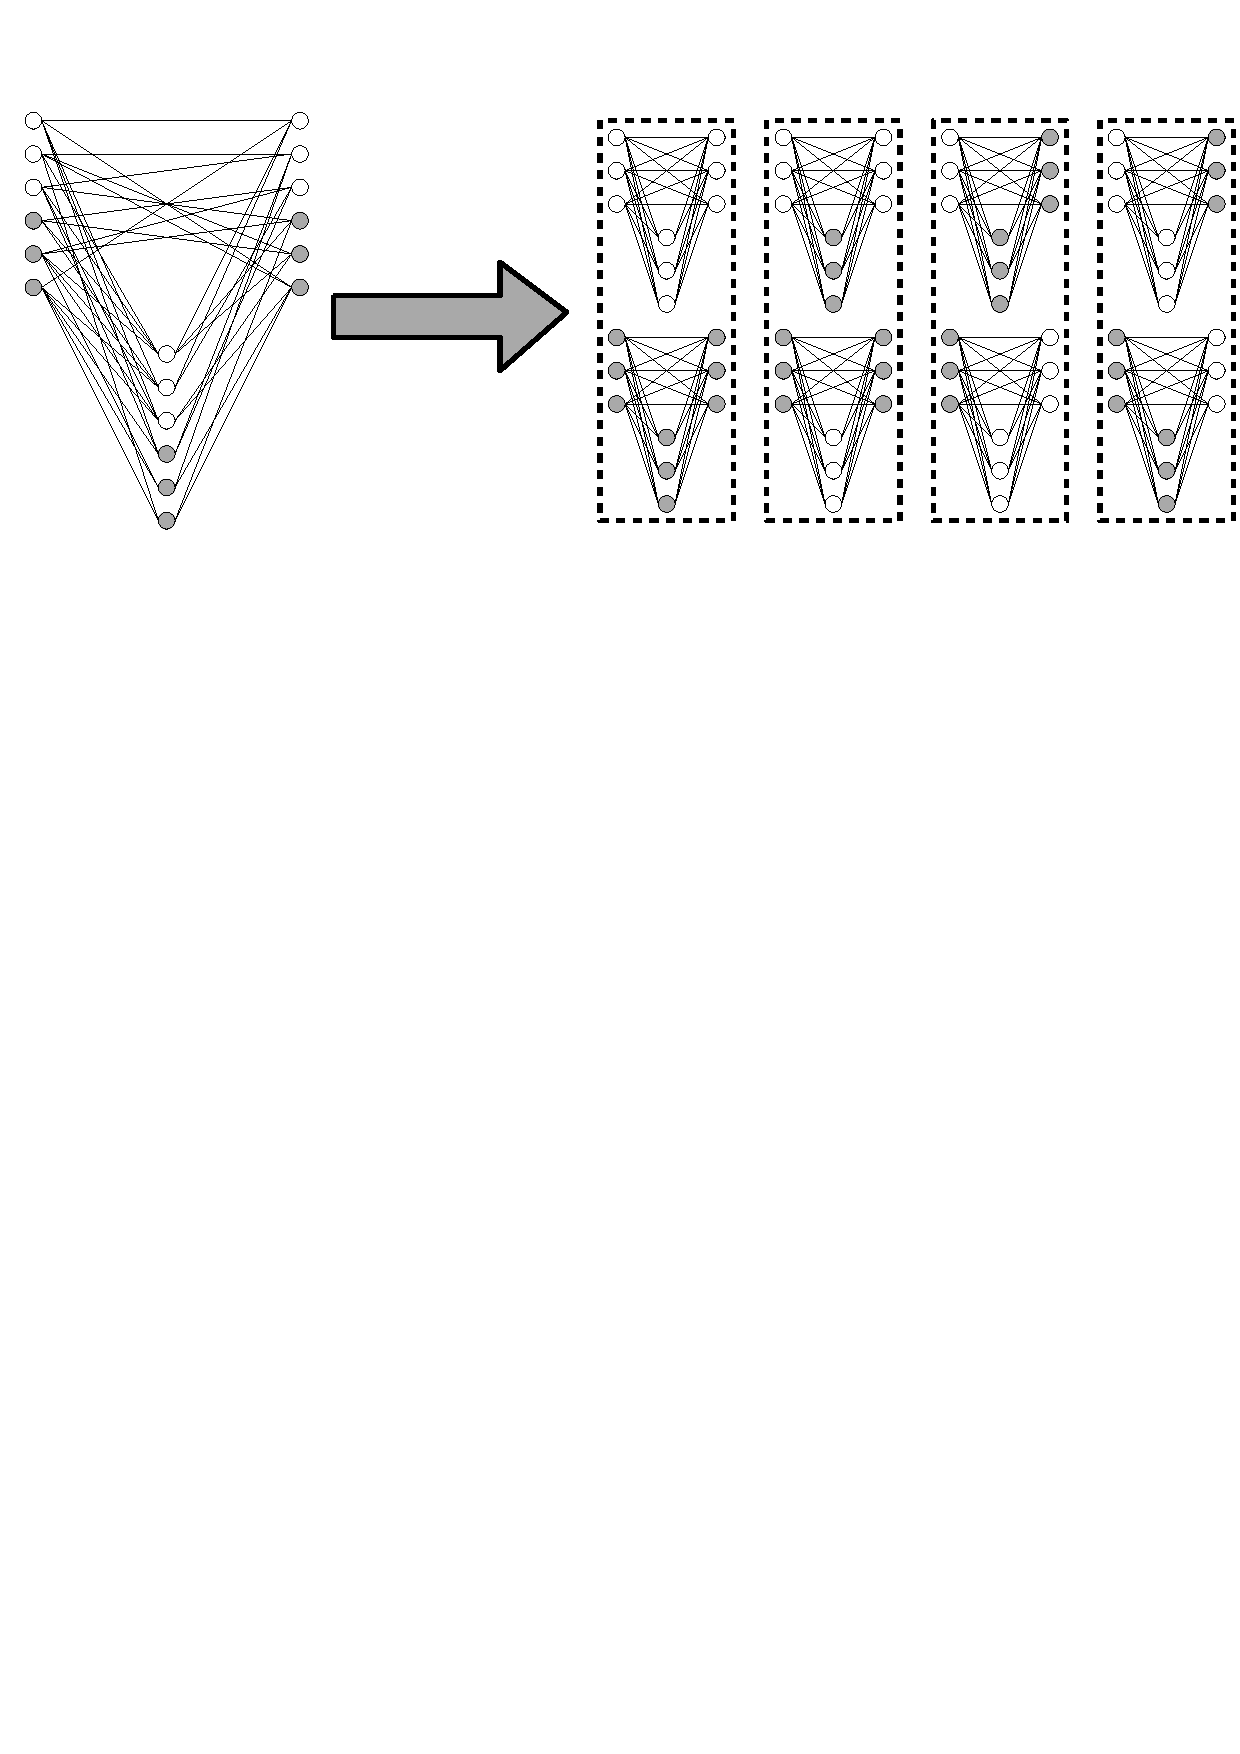
\includegraphics[scale=0.6]{fgcrypto/list-hard-fig.pdf}
		\caption{A depiction of splitting the subproblems for a case where $\ell=2$ and $k=3$.}
		\label{fig:listHardReduction}
	\end{figure}
	
	Note that producing these each of these $\ell$ instances is efficient, it takes time $O(n^2)$, which is just the input size.
	
	Next, we will show that the correct number of solutions are generated. 
	If $I$ has only one solution then exactly one $I_j$ in exactly one $S_{\vec{x}}$ has a solution. This is because any zero-$k$-clique in $I$ must involve exactly one node from each partition $P_i$. So, if there is one zero-$k$-clique it will only appear in subproblems where the node from partition $P_i$ is in  $P_i^j$ and $P^i_j$ appears in that subproblem. There is exactly one sub-problem generated with a specific choice of $k$ sub-partitions. So, exactly one $I_j$ in exactly one $S_{\vec{x}}$ has a solution.
	
	Let $S^*$ be the list $S_{\vec x}$ that contains a \zkclique. We have that the $S_{\vec{x}}$ which actually contains an instance with a solution is drawn from
	\[ \{I_1, \dots, I_x\}_{I_i \sim D_{1}, \land \forall j \neq i, I_j \sim D_{0}}.\]
	This distribution is exactly what we require for a list-problem. All that is left to show is if we have $\PFT{\ell \cdot n^k}$ adversary $\cA$ that can identify for which index $i$ there is a zero $k$-clique in $S^*$ (with probability at least 7/10), we can use $\cA$ to find the clique.
	
	%	By Lemma \ref{lem:TVDonesol} the original instance the distribution is within total variation distance of $n^k/R + n^{k-1}/R$ from planting a clique after uniformly at random picking the weight for each edge. 
	
	%	In the planted distribution, the instances in $S_{\vec{x}}$ which do not contain the planted clique have had their edges chosen uniformly at random. Thus, by Lemma \ref{lem:TVDnosol} they each have total variation distance $(n/g)^k/R$ from the distribution $D_{0}=D^{zkc}_{0}[R,n/g]$. 
	
	%	The instance which contains the planted solution itself had all edges chosen uniformly at random except for the planted clique edge. Thus, by Lemma \ref{lem:TVDonesol} it has total variation distance $(n/g)^k/R + (n/g)^{k-1}/R$ from $D_{1}= D^{zkc}_{1}[R,n/g]$. Which index within $S_{\vec{x}}$ this clique lands uniform over all the $g$ indices, because the clique nodes were picked uniformly at random. 
	
	%	The total error introduced by this process is $\leq g(n/g)^k/R+ (n/g)^{k-1}/R+n^k/R + n^{k-1}/R \leq 2n^k/R$ for $g>2$ and sufficiently large $n$. 
	%	
	%	We make no constraints on $g$ other than that $1<g<n$
	
	Now, recall that we are trying to solve a search problem: we need to be able to turn an index pointing to partitions into a witness for the original problem. According to the strong \zkclique~hypothesis, this search requires $O(n^k)$ time. However, as long as $\ell = n^{\Omega(1)}$, this is still faster in a fine-grained sense.
	
	On an input $I$ from $D_1$, algorithm $\cB$ uses $\cA$ as follows:
	\begin{itemize}
		\item Randomly partition each $P_i$ from $I$ into $\ell$ parts.
		\item For every $\vec x \in \Z_{\ell}^{k-1}$:
		\begin{itemize}
			\item Generate the list $S_{\vec x}$.
			\item Run $\cA(S_{\vec x})$ to get output $i$.
			\item Brute force search the size-$n^2$ \zkclique~instance $S_{\vec x}[i] = (P_1^i, \ldots, P_k^{i + x_k})$ for a solution. If one exists, output it, otherwise, continue.
		\end{itemize}
	\end{itemize}
	
	The first step only takes $O(\ell \cdot n)$ time since we are only divvying up $\ell n$ nodes. The second step requires a bit more analysis. The loop runs at most $\ell^{k-1}$ times. Each time the loop runs, it only takes $O(\ell \cdot n)$ time to construct $S_{\vec x}$, while $\cA$ takes $O((\ell \cdot n^{k})^{(1-\epsilon)})$ (since it is $\PFT{\ell \cdot n^k}$), and our brute force check takes $O(n^k)$ time. Putting this together, the algorithm takes a total time of 
	\[O(\ell \cdot n + \ell^{k-1} ((\ell \cdot n^{k})^{(1-\epsilon)} + n^k + \ell \cdot n) ) = O(\ell^{k-\epsilon}n^{k(1-\epsilon)} + \ell^{k-1}n^{k}) + \ell^k \cdot n.\]
	Both terms in this sum are strictly less than the hypothesized $\ell^k n^k$ time, and so $\cB$ is $\PFT{(\ell n)^k}$, contradicting the strong \zkclique~hypothesis.
	
	The reason we require $\ell(n) = n^{\Omega(1)}$ is because if it were less than polynomial in $n$, we would not get noticeable improvement through this method of splitting up the problem into several sub-problems --- the brute force step would take as long as solving the original problem via brute force.
	\qed
\end{proof}


\subsubsection{\zkclique~is Splittable}
Next we show that zero-k-clique is splittable. We start by proving this for a convenient range and then show we can use a reduction to get more arbitrary ranges. 

\paragraph{Splitting the problem over a convenient range.} Intuitively we will split the weights in half bit-wise, taking the first half of the bits of each edge weight, and then we take the second half of the bits of each edge weight to make another instance. If the $\binom{k}{2}$ weights on a $k$ clique sum to zero then the first half of all the weights sum to zero, up to carries, and the second half of all the weights sum to zero, also up to carries. We simply guess the carries. 

\newcommand{\high}[1]{{#1}^\uparrow}
\newcommand{\low}[1]{{#1}_\downarrow}
\newcommand{\ZkC}{\mathrm{Z}$k$\mathrm{C}}

\begin{lemma}
	\zkclique~is generalized splittable with error $\leq 4(\binom{k}{2} + 1) n^k/\sqrt{R}$ when $R=4^{x}$ for some integer $x$. 
	\label{lem:zkcSplitConvenientRange}
\end{lemma}
\begin{proof}
	We are given an instance of \zkclique~$I$ with $k$ partitions, $P_1, \ldots, P_k$ of $n$ nodes and with edge weights generated uniformly at random from $[0,R-1]$, where $R = 2^{2x}$ for some positive integer $x$.

	First we will define some helpful notation to describe our procedure.
	\begin{itemize}
		\item Let $\ZkC[R]$ denote the \zkclique~problem over range $R$.
		\item Let $w(P_i[a],P_j[b])$ be the weight of the edge in instance $I$ between the $a^{th}$ node in  $P_i$ and the $b^{th}$ node in $P_j$.
		\item Let $u$ be some number in the range $[0,R-1]$. Let $\high{u}$ be the high order $\lg(R)/2$ bits of the number $u$ (this will be an integer because $R$ is a power of 4). Let $\low {u}$ be the low order $\lg(R)/2$ bits of the number $u$.\\
		For the sake of notation, $\high w (P_i[a], P_j[b])$ denotes $\high{[w (P_i[a], P_j[b])]}$, and same for $\low w (P_i[a], P_j[b])$ denoting $\low {[w (P_i[a], P_j[b])]}$.
	\end{itemize}

	\newcommand{\lowI}{I_{low}}
	\newcommand{\highI}{I_{high}}
	Here is the reduction to take one instance of $\ZkC[R]$ and create a list of pairs of instances of $\ZkC[\sqrt R]$.
	%TODO: should put this in an algorithm
	\begin{enumerate}
		\item Take the $\ZkC[R]$ instance $I$ and create two instances of $\ZkC[\sqrt R]$, $\lowI$ and $\highI$ by the following:
		\begin{itemize}
			\item For every edge $(P_i[a], P_j[b])$ in $I$, let the corresponding edge in $\lowI$ have weight $\low w(P_i[a], P_j[b])$ and the edge in $\highI$ have weight $\high w(P_i[a], P_j[b])$.
		\end{itemize}
		\item For every $c \in [0,\binom k 2]$ (we need only check $\binom k 2$ possible carries):% because we are summing $\binom k 2$ numbers each of which are less than $1$):
		\begin{enumerate}
			\item Let $I_1^{c}$ be a copy of $\lowI$, but randomly permute all nodes.
			\item Let $I_2^{c}$ be a copy of $\highI$, but choose a random pair of a partitions $P_i$ and $P_j$: for all edges $e_2 \in I_2^{c}$ between $P_i$ and $P_j$, a copy of edge $e \in \highI$, let $w(e_2) = w(e) + c \mod \sqrt R$.
		\end{enumerate}
		\item Output the list $[(I_1^{(0)}, I_2^{(0)}), \ldots, (I_1^{(\binom k 2)}, I_2^{(\binom k 2)})]$
	\end{enumerate}
	For a visual aid, see figure \ref{fig:splittableRed} for a depiction of the splittable triangles. 

	\begin{figure}[h]
		\centering
		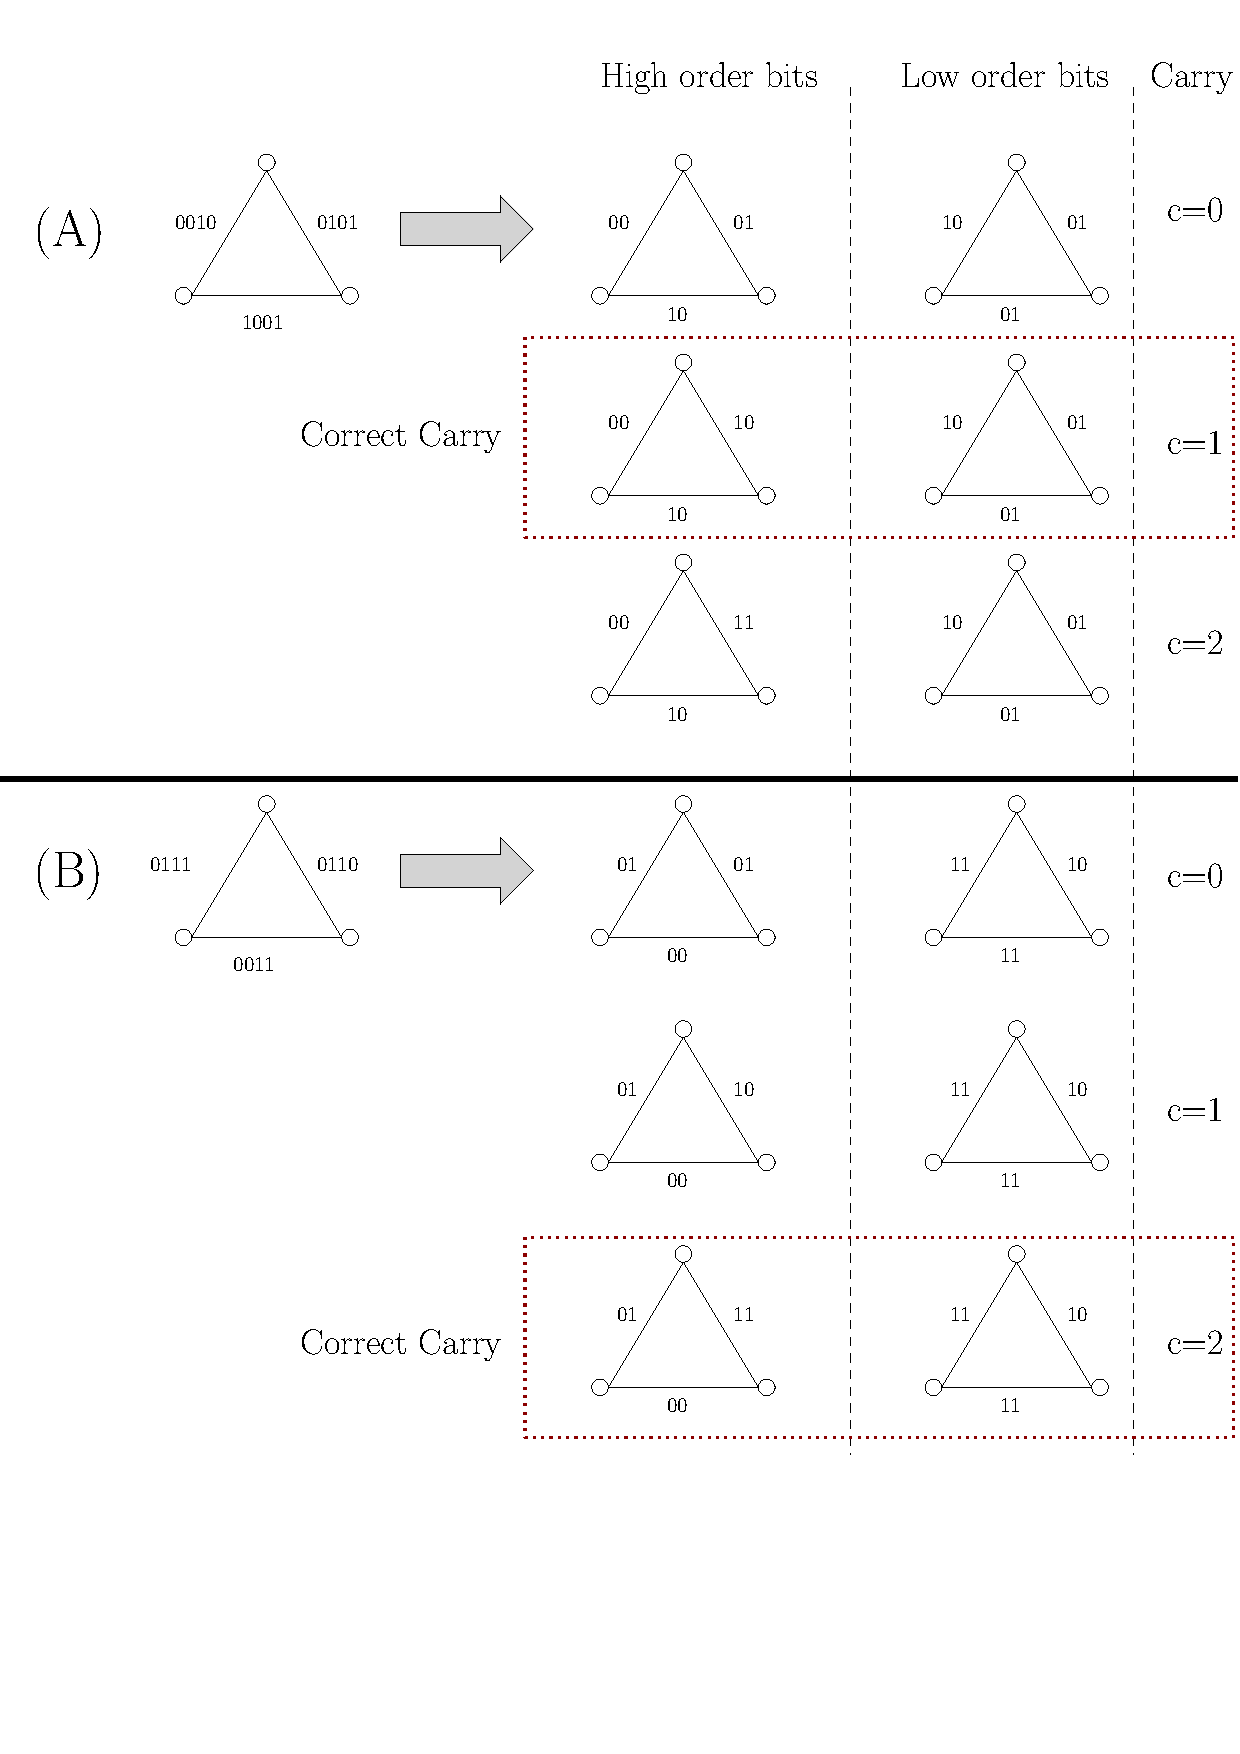
\includegraphics[scale=0.55]{fgcrypto/SplittableFig.pdf}
		\caption{An example of splitting the edges of triangles whose edges sum to $16$.}
		\label{fig:splittableRed}
	\end{figure}

	We will now show that we get the desired distributions in our list of instances depending on whether $I \sim D_0(\ZkC[R], n)$ or $I \sim D_1(\ZkC[R], n)$.
	\begin{itemize}
		\item $I \sim D_0(\ZkC[R], n)$. We need to show that every pair $(I_1^{(c)}, I_2^{(c)})$ is sampled from a distribution total variation distance $\le 2n^k/\sqrt R$ from $D_0(\ZkC[\sqrt R], n)^2$. Note that every pair is correlated very heavily with every other pair with respect to edge weights. But, within each pair, they are close to $D_0(\ZkC[\sqrt R], n)^2$.
		
		From lemma \ref{lem:TVDnosol}, this is TVD at most $\frac {n^k}{R}$ from just choosing edge-weights uniformly at random. So, consider $I' \sim \Generate(n,0)$, and do the same operations as for $I$ in the reduction: every bit in every edge weight will be chosen uniformly at random, meaning that the edge-weights in $\lowI'$ and $\highI'$ will also be uniform over $\sqrt R$. Permuting the nodes in $\lowI'$ does not change this distribution, and neither does adding (any) $c$ to a subset of edges in $\highI'$. Therefore, using lemma \ref{lem:TVDnosol}, \emph{both} $I_1'^{(c)}$ and $I_2'^{(c)}$ are TVD at most $\frac{n^k}{\sqrt R}$ from $D_0(\ZkC[\sqrt R], n)$. Since TVD is a metric, this implies that $I_1^{(c)}$ is TVD at most $n^k / \sqrt R$ from the distribution of $I_1'^{(c)}$, and thus at most $n^k / \sqrt R + n^k/ R$ from $D_0(\ZkC[\sqrt R], n)$ --- the same is true for $I_2^{(c)}$, even when conditioned on $I_1^{(c)}$. Therefore, the pair, for every $c$, is TVD at most $2(n^k / \sqrt R + n^k/ R) \le \frac{4 n^k}{\sqrt R}$.
		
		
		\item $I \sim D_1(\ZkC[R], n)$. We want to show that we get a list in which exactly one of the pairs of instances is distributed close to $D_1(\ZkC[\sqrt R], n)^2$.
		
		We will take a similar approach here, considering the planted distribution of $I$ instead of the true one. Let $I' \sim \Generate(n,1)$, so by lemma \ref{lem:TVDonesol}, $I'$ is TVD at most $2n^k/R$ from $D_1$. We will first show that $\lowI'$ is also drawn from a planted distribution over the range $\sqrt R$.
		Let $e'$ be the edge's weight that was changed to plant a zero clique. Now, for every edge except $e'_{low}$, the edges of $\lowI'$ are distributed uniformly. $e'$ is a randomly chosen edge corresponding to a randomly chosen clique in $I'$, and therefore $e'_{low}$ is also a randomly chosen edge corresponding to a randomly chosen clique in $\lowI'$. The act of making that clique sum to 0 mod $R$ also requires that the low-order bits sum to $0$ mod $\sqrt R$ --- otherwise the high-order bits cannot cancel out anything left over. Therefore, by setting $w(e')$ to the value making the clique sum to 0, we are exactly planting a clique in $\lowI'$. This distribution has TVD $\le \frac{2n^k}{\sqrt R}$ from $D_1(\ZkC[\sqrt R], n)$. Because $I_1'^{(c)}$ is just a permutation on the nodes of $\lowI'$ for every $c$, $I_1'^{(c)}$ will have TVD at most $\frac{2n^k}{\sqrt R}$ from $D_1$ as well.
		
		Now, we need that at least one of the pairs in this list to be close to $D_1(\ZkC[\sqrt R], n) \times D_1(\ZkC[\sqrt R], n) $. It will turn out that there exists a $c$ such that $I_2'^{(c)}$ will also be close to $D_1$ (whereas $I_1'^{(c)}$ is distributed close to $D_1$ for every $c$). Let $c^*$ be the correct carry --- that is for the clique planted in $I'$, $\sum_{e \in clique} \low w(e) = \sqrt R c^* \mod R$. Now, without loss of generality, we can assume that in the plant of $I'$, the edge $e^*$ chosen to complete the zero-$k$ clique was between partitions $P_i$ and $P_j$. So, considering every other edge in $I_2'^{(c^*)}$, it is distributed uniformly at random (adding $c^*$ will not change that distribution). Now, for that special clique $C^*$ that was planted in $I'$, we have that
		\begin{align*}
		\sum_{e \in C^*} w(e) &= \sqrt R \cdot \sum_{e \in C^*} \high w(e) + \sum_{e \in C^*} \low w(e)\\
		&= \sqrt R (\sum_{e \in C^*} \high w(e) + c^*)\\
		&= \sqrt R (\high w(e^*) + c^* + \sum_{e \in C^*, e \neq e^*} \high w(e)) = 0 \mod R
		\end{align*}
		Since the quantity $\sqrt R (\high w(e^*) + c^* + \sum_{e \in C^*, e \neq e^*} \high w(e))$ is 0 mod $R$, then $\high w(e^*) + c^* + \sum_{e \in C^*, e \neq e^*} \high w(e) = 0 \mod \sqrt R$.
		
		This means that $I_2'^{(c^*)}$ is drawn from $\Generate(n,1)$ over the range $\sqrt R$. Since TVD is a metric, we have that for $I \sim D_1(\ZkC[\sqrt R], n)$ (TVD at most $\frac {n^k}{R}$ from $\Generate(n, 1)$), there exists a $c^*$ such that $I_2^{(c^*)}$ is TVD at most $\frac{2n^k}{\sqrt R}$ from $D_1$ --- even when dependent on $I_1^{(c^*)}$. Therefore, the TVD of $(I_1^{(c^*)}, I_2^{(c^*)}) = \Split(I)$ to $D_1^2$ is at most $\frac{4 n^k}{\sqrt R}$.
	\end{itemize}
	Therefore, when $I \sim D_0(\ZkC[R], n)$, we get a list of pairs of instances TVD $\le 4n^k / \sqrt R$ from $D_0(\ZkC[R], n)^2$; the probability that any of these pairs here err is $\le(\binom k 2 + 1) \cdot \frac{4n^k}{\sqrt R}$ by a union bound. Similarly, when $I \sim D_1(\ZkC[R], n)$, we get there exists a pair in this list of the form $D_1(\ZkC[R], n)^2$; the probability of erring here is $\le \frac{4 n^k }{\sqrt R}.$
	
	Therefore, the total error here is $\le (\binom k 2 + 1) \cdot \frac{4n^k}{\sqrt R}$.
	\qed
\end{proof}

\paragraph{\zkclique~is Splittable Over Any Large Enough Range.}\label{sec:zkcsplittable}
Our techniques also generalize to any large enough range (even ones not of the form $4^x$). For example, if you believe that the problem is hard only over a prime range, we can prove that as well. As stated, our error is $\binom{k}{2}4^{\binom{k}{2}}3 n^k/\sqrt{R} = O(n^k/\sqrt R)$. For this to be meaningful, $R = \Omega(n^{2k})$, and in our constructions, $R$ is $\Omega(n^{6k})$. We will show in the next section why the zero $k$-clique problem is still hard over these larger ranges.

\begin{theorem}
	Zero-k-clique is generalized splittable over any range $R$, with error $\leq \binom{k}{2}4^{\binom{k}{2}}3 n^k/\sqrt{R}$. 
	\label{thm:zkcsplittable}
\end{theorem}
%TODO: go through that proof, too. is this statement correct?
\begin{proof}
	Given an instance $I$ with range $R$ we will produce $\leq \binom{k}{2}4^{\binom{k}{2}}$ instances, corresponding to guesses over what ranges the clique edge weights fall into. 
	
	Take the next smallest power $R' = \max\{2^{2x}| 2^{2x}<R \text{ and } x\in \mathbb{Z} \} $. 
	Now let $c = \lceil R/R' \rceil$. We will now create $c$ subsets of $R$ each of size $R'$.  $S_i = [R'i,R'(i+1)-1]$ for $i\in [0,c-2]$ and $S_{c-1} = [R-R' , R-1]$. Note that these subsets completely cover the range $[0, R-1]$ and are each of size $\le R'$. Let $\Delta_i = R'i$ for $i\in [0,c-2]$ and $\Delta_{c-1} = R-R'$. 
	
	Let the partitions of $I$ be $P_1, \ldots, P_k$. Let the set of edges between $P_i$ and $P_j$ be $E_{i,j}$. For all $i,j$ pairs $i\ne j$ we will choose a number between $[0,c-1]$. Call these numbers $g_{i,j}$ and the full list of them $\vec{g}$. For all possible choices of $\vec{g} \in \mathbb{Z}_{c}^{\binom{k}{2}}$ and $d \in [0, \binom{k}{2}-1]$ we will generate an instance $I_{\vec{g},d}$ over range $R'$ as follows: 
	
	For edge set $E_{i,j}$ that isn't $E_{1,2}$, for every edge in that edge set $e \in E_{i,j}$ if the weight of $e$, $w(e) \in S_{g_{i,j}}$ then set $w_{\vec{g},d}(e) = w(e) \mod R'$, if $w(e) \nin S_{g_{i,j}}$ then set $w_{\vec{g},d}$ to be a weight chosen uniformly at random from $[0, R'-1]$. Now note that these values are completely uniform over the range from $[0,R'-1]$. 
	
	For $E_{1,2}$ , for every edge in that edge set $e \in E_{1,2}$ if the weight of $e$, $w(e) \in S_{g_{1,2}}$ then set $w_{\vec{g},d}(e) = w(e) + dR \mod R'$, if $w(e) \nin S_{g_{1,2}}$ then set $w_{\vec{g}}$ to be a weight chosen uniformly at random from $[0, R'-1]$. Now note that these values are also completely uniform over the range from $[0,R'-1]$. 
	
	If no clique existed in the original instance then the chance that one is produced here is bounded by $n^k/R' \leq n^k4/R'$ by Lemma \ref{lem:TVDnosol}. Because we make so many queries this chance that any of them induce a clique is $\leq \binom{k}{2}4^{\binom{k}{2}}n^k4/R'$. 
	
	If the original instance was drawn from $D^{zkc}_{1}[R,n]$ then by Lemma \ref{lem:TVDonesol} this is only $\leq n^k/R + n^{k-2}/R$ total variation distance away from the instance generated by choosing each edge at random and then planting a clique. Then the procedure produces uniformly looking edges except for the planted edge. In the generated instance where the original zero clique edge weights are in $\vec{g}$ and the zero k-clique sums to $dR$ then the instance $I_{\vec{g},d}$ will have that planted edge set to the value such that zero k-clique from the original is a planted instance. So, that produced instance is drawn from a distribution with total variation distance $\leq n^k/R' + n^{k-2}/{R'}$ from $D^{zkc}_{1}[R',n]$. 
	
	Then we use the splitting procedure from Lemma \ref{lem:zkcSplitConvenientRange} to generate two instances from each of our generated instances. The probability of a no instance becoming a yes instance is $\leq \binom{k}{2}4^{\binom{k}{2}}3 n^k/\sqrt{R}$, if there is a yes instance then it will generate a yes instance and have total variation distance at most $\leq \binom{k}{2}4^{\binom{k}{2}}3 n^k/\sqrt{R}$ from $D^{zkc}_{1}[\sqrt{R'},n]^2$. \qed
\end{proof}

%%\subsection{Larger Ranges for \zkclique~are as Hard as Smaller Ranges.}
%We note that our constructions work for a large range: $R = \Omega(n^{6k})$. This theorem states that finding zero $k$-cliques over smaller ranges is as hard as finding them over larger ones.
%So, if you believe that \zkclique~is hard over a range where an uniformly sampled instance is expected to have one solution (e.g. a small range like $O(n^k)$), we can show that this implies larger ranges, which are used extensively in our constructions, are also hard.
%
%\begin{theorem}
%	\Strongzkc for range $R=n^{c k}$ is implied by the \RandomZKC if $c>1$ is a constant.
%	\label{thm:rangeExtendThm}
%\end{theorem}
%\begin{proof}
%	Create $n^{(1-1/c)}$ random partitions of the nodes where each partition is of size $n^{1/c}$. Then generate $n^{(1-1/c)k}$ graphs by choosing every possible choice of $k$ partitions.
%	
%	This results in $n^{(1-1/c)k}$ problems of size  $n^{1/c}$ with range $n^k$. 
%	
%	If an algorithm $A$ violated \Strongzkc for range $n^{c k}$ then it must have some running time of the form $O(n^{k-\delta})$ for $\delta > 0$. We could run $A$ on all $n^{(1-1/c)k}$ problems, resulting in a running time of $n^{k/c-\delta/c}n^{(1-1/c)}k = O(n^{k-\delta/c})$ for the Random Edge problem. If we find a valid zero-$k$-clique then we return $1$. If we don't we return $0$ with probability $1/2$ and $1$ with probability $1/2$.
%	
%	Let $p_1$ be the probability that any one of the $n^{k/c}$ has exactly one zero clique, conditioned on $val(I)=1$ (that there is at least one solution). 
%	
%	If \Strongzkc is violated then we return the correct answer with the probability at least $p_1 \frac{1}{100} + (1-p_1/100)/2 = 1/2+p_1\frac{1}{200}$. So, we now want to lower bound the value of $p_1$. 
%	
%	%Let $p_0'$ ,$p_1'$ and $p_{\geq 2}'$ be the probabilities that a single instance of size $n^{k/c}$ has zero, one or at least two cliques respectively.
%	
%	The probability that there are more than $2$ cliques in a subproblem of size  $n^{1/c}$, conditioned on there being at least one clique is at most $n^{-k(1-1/c)}$. Because to generate the distribution of problems of size $n^{1/c}$ with at least one clique one can plant a clique (randomly choose $k$ nodes and randomly choose $\binom{k}{2}-1$ edge weights, then choose the final edge weight such that this is a zero $k$-clique). The expected number of cliques other than the planted clique is $\frac{n^{1/c}-1}{n^k}$ and the number of cliques other than the planted clique is a non-negative integer.
%	
%	So conditioned $val(I)=1$ we have that $p_1\geq 1-n^{-k(1-1/c)}$. So the probability of success, conditioned on $val(I)=1$  is at least $p_1/100 \geq 1/200$.
%	
%	%So 
%	%$$(p_1'+p_{\geq 2}')n^{-k(1-1/c)}\geq p_{\geq 2}'.$$ 
%	%Which means 
%	%$$2p_1' n^{-k(1-1/c)} \geq p_1' \frac{n^{-k(1-1/c)}}{1-n^{-k(1-1/c)}} \geq p_{\geq 2}'.$$
%	
%	%We finally 
%	
%	%We will now determine how often we are correct. Let $p_0$, $p_1$ and $p_{\geq 2}$ be the probability that the original instance has $0$, $1$ or at least $2$ zero-$k$-cliques respectively. 
%	
%	%The probability that there are more than $2$ cliques in a subproblem of size  $n^{1/c}$, conditioned on there being at least one clique is $\leq n^{-k(1-1/c)}$. To generate the distribution of problems of size $n^{1/c}$ with at least one clique one can plant a clique (randomly choose $k$ nodes and randomly choose $\binom{k}{2}-1$ edge weights, then choose the final edge weight such that this is a zero $k$-clique). The expected number of cliques other than the planted clique is $ n^{-k(1-1/c)}$ and the number of cliques other than the planted clique is a non-negative integer. 
%	
%	%We have that $p_0+p_1+p_{\geq 2}=1$ and $p_1\geq p_{\geq 2} n^{-k(1-1/c)}$. So $p_0+p_1\geq 1-n^{-k(1-1/c)}$.
%	
%	
%	%We add error $n^{-k(1-1/c)}$, however, this is $o(\frac{1}{\lg(n)})$.
%\end{proof}

\section{Fine-Grained One-Way Functions}\label{sec:fg-owfs}
% !TEX root = ../main.tex

%\section{Fine-Grained One-Way Functions}\label{sec:fg-owfs}

In this section, we give a construction of fine-grained OWFs (FGOWF) based on plantable $T(n)$-\ACIH~problems. We first show that even though the probability of inversion may be constant (we call this ``medium'' fine-grained one-way), we can do some standard boosting in the same way weak OWFs can be transformed into strong OWFs in the traditional sense. Then, given such a plantable problem, we will prove that $\Generate(n,1)$ is a medium $T(n)$-FGOWF. Then, from this medium FGOWF, we can compile a strong FGOWF using this boosting trick. Then, since \zkclique~is plantable (see Theorem \ref{thm:zkcPlantable}), this implies that assuming \zkclique~is hard yields fine-grained OWFs.

Finally, we discuss the possibility of fine-grained hardcore bits and pseudorandom generators. It turns out that the standard Goldreich-Levin \cite{hardCoreBitsAndXorLemmaFromGL} approach to creating hardcore bits works in a similar fashion here, but requires some finessing; it will not work for \emph{all} fine-grained OWFs.

We will be using $\tilde{O}(\cdot)$ to suppress sub-polynomial factors of $n$ (as opposed to only $\lg(n)$ factors). 

\subsection{Weak and Strong OWFs in the Fine-Grained Setting}

Traditional cryptography has notions of weak and strong OWFs. Weak OWFs can be inverted most of the time, but a polynomial-fraction of the time, they cannot be. These weak OWFs can be compiled into strong OWFs (showing that weak OWFs imply strong OWFs), where there is a negligible chance that the resulting strong OWF is invertible over the choice of inputs.

Here we will briefly define ``medium'' $T(n)$-FGOWFs, and show how they can imply a ``strong'' $T(n)$-FGOWF, where ``strong'' refers to definition \ref{def:fg-owf}

\begin{definition}
	A function $f$ is a medium $T(n)$-FGOWF if there exists a sub-polynomial function $Q(n)$ such that for all $\PFT{T(n)}$ adversaries $\cA$,
	\[ \Pr_{x \getsr \{0,1\}^n}\bigl[ \cA(f(x)) \in f\inv(f(x)) \bigr] \le 1 - \frac 1 {Q(n)}. \]
\end{definition}

\begin{claim}\label{clm:medium-strong-owf}
	Medium $T(n)$-FGOWFs imply strong $T(n)$-FGOWFs for any polynomial $T(n)$ that is at least linear.
\end{claim}
\begin{proof}
	The structure of this proof will follow Yao's original argument augmenting weak OWFs to strong ones. Intuitively, we are able to use this argument because sub-polynomial functions compose well with each other.
	
	Assume for the sake of contradiction that no strong $T(n)$-FGOWF exists. Then, there exists some function $p’(n)$ such that $p’(n)$ is sub-polynomial and for all functions $f$ computable in $T(n)^{1-\epsilon}$ time there exists a $PFT_{T(n)}$ adversary that can invert the function $f$ with probability $1-\frac{1}{p’(n)}$.
	
	Let $f$ be a medium $T(n)$-FGOWF, where the probability any $\PFT{T(n)}$ adversary inverts it is $1 - \frac 1 {Q(n)}$. The basic idea will be to produce $g$ that is just a concatenation of many $f$s, just as in the traditional cryptographic case.
	
	For any positive-integer function $c(n)$, let $g(x_1 || \dots || x_{c(n)}) = f(x_1)||$ $\dots ||f(x_{c(n)})$, where $||$ denotes concatenation.
	Let $c(n) = 4 \left( Q(n)r(n) \right)^2$ (or the ceiling of $4 \left( Q(n)r(n) \right)^2$, if not an integer). 	Where $r(n)$ is a subpolynomial function such that $r(n) \ge p’(c(n) \cdot n)$. Note that $p’(n)$ is subpolynomial, and that as a result some such function $r(n)$ exists. Specifically, setting $r(n) = p'(n^2)$ satisfies both criteria.
	
	Now note that $c(n) \cdot n = \~O(n)$, and so $T(c(n) \cdot n) = \~O(T(n))$. Furthermore, $g$ is a $T(c(n) \cdot n) = O(T(n))$-FGOWF since $c(n)$ is subpolynomial.
	
	Now, for sake of contradiction, let $\cA$ be a $\PFT{T(n)}$ such that there exists a subpolynomial function $p'$ where
	\[\Pr\bigl[\cA(g(x_1 || \dots || x_c)) \in g^{-1}(g(x_1 || \dots || x_c))\bigr] \ge \frac 1 {p'(c(n) \cdot n)}.\]
	
	
	Let $p(n) = p'(c(n) \cdot n)$. Because $c(n)\cdot n = O(n^2)$ and $p'(n)$ is sub-polynomial, $p'(c(n) \cdot n) = p(n)$ is also sub-polynomial. Therefore,
	\[\Pr\bigl[\cA(g(x_1 || \dots || x_c)) \in g^{-1}(g(x_1 || \dots || x_c))\bigr] \ge \frac 1 {p(n)}.\]

	We will define a $\PFT{T(n)}$ function $\cA_0$ that makes a single call to $\cA$: on input $y = f(x)$
	\begin{enumerate}
		\item Choose $i \getsr [c(n)]$.
		\item Let $z_i = y$
		\item For all $j \in [c(n)]$, $j \neq i$, $x_j \getsr \{0,1\}^n$ and $z_j = f(x_j)$.
		\item Run $\cA$ on $(z_1, \dots, z_{c(n)})$ to get output $(x_1, \dots, x_{c(n)})$ if $\cA$ succeeds.
		\item If $\cA$ succeeded, output $x_i$.
	\end{enumerate}
	
	Because all operations in $\cA_0$ are either calling $\cA$ (once) or take time $O(n\cdot c(n))$,\footnote{It does not make much sense for $T(n)$ to be sublinear for our contexts} $\cA_0$ is a $\PFT{T(n)}$ algorithm. Now, we will let $\cB$ be an algorithm calling $\cA_0$ $d(n) = 4c(n)^2 (n)p(n)Q(n)$ times, returning a valid inversion of $f(x)$ if $\cA$ succeeded at least once.
	
	We will call $x \in \{0,1\}^n$ 'good' if $\cA_0$ inverts it with probability at least $\frac 1 {2c^2(n)p(n)}$; $x$ is 'bad' otherwise. Notice that if $x$ is good, then $\cB$, which runs $\cA$ many times, succeeds with high probability:
	
	\[ \Pr\left[\cB(f(x)) \mbox{ fails} | x\mbox{ is good}\right] \le \left(1 - \frac 1{2c^2(n)p(n)}\right)^{d(n)} \sim e^{-2Q(n)} < \frac 1 {2Q(n)}. \]
	
	
	We will show that there are at least $2^n(1 - \frac{1}{2p(n)})$ good elements.
	
	
	\begin{claim}
		There are at least $2^n(1 - \frac{1}{2p(n)})$ good elements.
	\end{claim}
	\begin{proof}
		For a contradiction, assume there are at least $2^n(\frac{1}{2p(n)})$ bad elements. We will end up contradicting the inversion probability of $\cA$ (which is at least $1/p(n)$). For notation, let $\vec x = (x_1, \dots, x_{c(n)}) \in \{0,1\}^{n\cdot c(n)}$, and $\vec x$ will be chosen uniformly at random over the input space.
		\begin{align*}
		\Pr_{\vec x}[\cA(\vec z = g(\vec x)) \mbox{ succeeds}] &= \Pr[\cA(\vec z)\mbox{ succeeds} \land \exists \mbox{bad }x_j]\\
		&\qquad + \Pr\left[\cA(\vec z)\mbox{ succeeds} \land \mbox x_j \mbox{ good }\forall j \in [c(n)] \right]
		\end{align*}
		
		Now, for all $j \in [c(n)]$,
		\begin{align*}
		\Pr_{\vec x}[\cA(\vec z) \mbox{ succeeds} \land x_j\mbox{ is bad}] &\le \Pr_{\vec x}[\cA(\vec z) \mbox{ succeeds} |  x_j\mbox{ is bad}]\\
		%\cdot \Pr_{x_j}[ x_j\mbox{ is bad}]\\
		&\le c(n) \Pr_{\vec x}[\cA_0(f(x_j))\mbox{ succeeds} | x_j\mbox{ is bad}]\\
		&\le \frac{c(n)}{2c^2(n)p(n)} = \frac{1}{2c(n)p(n)}
		\end{align*}
		So, if we just union bound over all $j$, we get
		\[ \Pr_{\vec x}[\cA(\vec z) \mbox{ succeeds} \land \mbox{some } x_j \mbox{ are bad}] \le \sum_{j = 1}^{c(n)} \Pr_{\vec x}[\cA_0(f(x_j))\mbox{ succeeds} \land x_j\mbox{ is bad}] \le \frac{1}{2p(n)}. \]
		

		
		And one more quick upper bound yields
		
		\begin{align*}
	\Pr[\cA(\vec z) \mbox{ succeeds} \land \mbox{all } x_j \mbox{ are good}] &\le \Pr_{\vec x}[\mbox{all $x_j$ good}]\\
	&< \left(1 - \frac{1}{2p(n)}\right)^{c(n)}\\
	&\leq e^{-2\left(Q(n)r(n)\right)^2 / p(n)}\\
	&\leq e^{- 2\left(Q(n)\right)^2 \cdot p(n)} < \frac 1 {2p(n)}.
		\end{align*}
		
		Finally, this yields the contradiction to the claim that there are at least $2^n(\frac{1}{2p(n)})$ bad elements:
		\begin{align*}
		\Pr_{\vec x}[\cA(\vec z) \mbox{ succeeds}] < \frac{1}{p(n)}.
		\end{align*}\qed
	\end{proof}

	Note that $p(n)\geq Q(n)$ because $1/Q(n)$ is the maximum probability of inverting a single copy of $f(\cdot)$, where as $1/p(n)$ is assumed (for contradiction) to be the probability that a function inverts $c(n)$ copies of $f(\cdot)$ simultaneously. So, there are at most $2^n(\frac{1}{2Q(n)})$ bad elements.

	Now that we know there is a high probability that we hit a good $x$, we can finish the rest of this proof.
	\begin{align*}
	\Pr_{x}[\cB(f(x)) \mbox{ fails}] &= \Pr[\cB(f(x)) \mbox{ fails} | x \mbox{ is good}] \Pr_x[x \mbox{ is good}]\\
	&\qquad + \Pr[\cB(f(x)) \mbox{ fails} | x \mbox{ is bad}] \Pr_x[x \mbox{ is bad}]\\
	&\le\Pr[\cB(f(x)) \mbox{ fails} | x \mbox{ is good}] \Pr_x[x \mbox{ is good}] + \Pr_x[x \mbox{ is bad}]\\
	&\le \frac{1}{2Q(n)}\left(1 - \frac 1 {2Q(n)}\right) + \frac{1}{2Q(n)} < \frac 1 {Q(n)}
	\end{align*}
	Thus, the chance that $\cB$ actually has of inverting $f$ is strictly greater than $1 - \frac 1 {Q(n)}$, contradicting the claim that $f$ was medium-hard with respect to $Q(n)$.\qed
\end{proof}

\paragraph{Weaker Fine-Grained OWFs.} Now, because we are in the fine-grained setting, we can talk about gaps. There is a notion of weak-OWFs in cryptography where we can say if there exists \emph{any} polynomial such that we can invert with probability $1 - 1/\poly$, we can construct strong OWFs. We want a similar notion for fine-grained OWFs. Here we can't just choose any polynomial --- we have to choose a polynomial that respects the gap.

Formally, for an $T(n)$-FGOWF $f$ that has $\PFT{T(n)}$ adversaries inverting it with probability $1 - 1/P(n)$ for some $P(n)$, we can get that a $\PFT{T(n)}$ adversary can invert $f$ with probability $(1 - 1/P(n))^{c(n)}$. Now, as long as there exists $\delta'$ such that $T(n)^{1-\delta}P(n) = T(n)^{1-\delta'}$, there is still a gap ($\delta' < \delta$) even if we compute $f$ $P(n)$ times to evaluate $f$. Therefore, we are able to get a strong fine-grained OWF from a weak one, as long as it's not \emph{too} weak.

\subsection{Building Fine-Grained OWFs from Plantable Problems}\label{sec:building-fgowfs}

Here we show that one can generate fine-grained one way functions from plantable problems. Recall the definition of Plantable states that there exists an algorithm $\Generate(n,b)$ where when $b=0$, an instance of the problem \emph{without} a solution is generated, and when $b=1$, an instance of a problem \emph{with one} solution is generated with probability at least $1 - \epsilon$. This probabilistic element, $\epsilon$, is actually a bound on the total variation distance of the distributions we are actually aiming to sample from: $\Generate(n,0)$ and $\Generate(n,1)$ have total variation distance at most $\epsilon$ from $D_0(P,n)$ and $D_1(P,n)$ respectively.

\begin{theorem}\label{thm:FGOWFs-exist}	%\label{thm:plantableOWF}
	If there exists a Plantable $T(n)$-\ACIH~problem where $G(n)$ is $\PFT{T(n)}$ with error some constant $\epsilon < 1/3$, then $T(n)$-FGOWFs exist.
	\footnote{We would like to thank Chris Brzuska and his reading group for finding a bug in the original version of this proof. To correct this bug, we added the word `constant' to the theorem statement, removed our severe abuse of notation, and fixed the proof accordingly.}
\end{theorem}
\begin{proof}
	Let $P$ be a Plantable $T(n)$-\ACIH~problem where $G(n) = T(n)^{1-\delta}$ for some constant $\delta>0$. So, the (randomized) algorithm $\Generate(n,1)$ is $\PFT{T(n)}$ and outputs an instance $I$ that has at least one solution --- we write this as $\Generate(n,1; r)$ when explicitly noting which randomness was used.
	
	We want to show that being able to invert $\Generate(n,1; r)$, over the distribution from $r$, in a fine-grained sense, as solving the \ACIH~problem $P$. Let $\epsilon$ be the upper bound on the total variation distance between $\Generate(n,1)$ and $D_1(P,n)$, as per Definition \ref{def:plantable}.
	
	For sake of contradiction, assume that no \emph{medium} $T(n)$-FGOWF exist. So, we can invert $\Generate(n,1)$ with any probability $1 - \frac 1 {Q(n)}$ for any sub-polynomial $Q(n)$. Let $\cA$ be a $\PFT{T(n)}$ algorithm that inverts $\Generate(n,1)$ with probability $\gamma > 1 - \frac{1}{\log(n)}$ (note that $\log(n)$ is significant). We will show that this violates the assumption that $P$ is a $T(n)$-\ACIH~problem.
	
	We now construct a $\PFT{T(n)}$ algorithm $\cB$ that distinguishes between $I \sim D_0(P,n)$ and $I \sim D_1(P,n)$ with probability greater than $2/3$, violating the hardness assumption on $P$.
	\begin{itemize}
		\item Given $I$ from distribution $D$, $\cB$ gives $I$ to $\cA$.
		\item $\cA$ outputs $r$.
		\item If $\Generate(n,1;r) == I$, output $1$. Otherwise, output $0$.
	\end{itemize}
	
	
	%Andrea Edit
	We will now compute the probability that $\cB$ distinguishes between inputs from $D_1$ and $D_0$. Recall that $D$ is just sampling with $D_0$ with probability $1/2$, and otherwise samples from $D_1$. For the sake of brevity let the notation $I \in D_0$ and $I\in D_1$ convey that $I$ is in the support of $D_0$ and the support of $D_1$ respectively. We have
	\begin{align*}
	\Pr_{I \sim D}[\cB(I)\mbox{ distinguishes }D_0\text{ from }D_1] &= \Pr_{I \sim D_1}[\cB(I) = 1] \cdot \Pr_{I \sim D}[I \in D_1] \\
	&\qquad + \Pr_{I \sim D_0}[\cB(I) = 0]\cdot \Pr_{I \sim D}[I \in D_0]\\
	&= \frac 1 2 \Pr_{I \sim D_1}[\cB(I) = 1] + \frac 1 2 \Pr_{I \sim D_0}[\cB(I) = 0].
	\end{align*}
	First, we note that $\Pr_{I \sim D_0}[\cB(I) = 0] = 1$ because $\Generate(n,1; r)$ is guaranteed to produce a witness for all randomness $r$. This means that any $I$ sampled from $D_0$ is not in the image of $\Generate(n,1)$, and therefore, $\cA$ cannot produce a valid inverse.
	
	Then, we use the fact that $D_1$ is close in total variation distance to $\Generate(n,1)$ to show that $\Pr_{I \sim D_1}[\cB = 1] \ge \gamma - 2\epsilon$. Let $p_{G_1}$ be the pdf of $\Generate(n,1)$ and $p_{D_1}$ be the pdf of $D_1$. Let $\cI$ be the set of all instances of the problem. Let $S = \{I \in \Img(\Generate(n,1)) : \Generate(n,1;\cA(I)) = I \}$ be the set of instances produced by $\Generate$ that $\cA$ can successfully invert. Recall that $\TVD(D_1, \Generate(n,1)) \leq \epsilon$ means $\sum_{I \in \cI} \vert p_D(I) - p_G(I) \vert \leq 2 \epsilon$ by the definition of $\TVD$.
	\begin{align*}
	2\epsilon &\ge \sum_{I \in \cI} \vert p_{D_1}(I) - p_{G_1}(I) \vert\\
	&\ge \sum_{I \in S} \vert p_{D_1}(I) - p_{G_1}(I) \vert \\
	&\ge \sum_{I \in S} \left[p_{D_1}(I) \right] - \sum_{I \in S} \left[p_{G_1}(I) \right].
	\end{align*}
	This implies $ \sum_{I \in S} \left[p_{G_1}(I) \right] \ge \sum_{I \in S} \left[p_{D_1}(I) \right] - 2\epsilon$, and therefore $\Pr_{I \sim D_1}[\cB = 1] \ge \gamma - 2\epsilon$.
	
		
	%Andrea Edit
    Notice that since $\epsilon$ is constant and less than $\frac 1 3$, $\frac 1 3 - \alpha = \epsilon$ for some constant $\alpha>0$.
	Putting this together, we have that
	\begin{align*}
	\Pr_{I \sim D}[\cB(I)\mbox{ distinguishes }D_0\text{ from }D_1] &\ge \frac 1 2 \cdot (\gamma - 2\epsilon) + \frac 1 2\\
	&= \frac \gamma 2 - \epsilon + \frac 1 2\\
	&= 1 - \frac{1}{2\log(n)} - \epsilon\\
	&\ge 1 - \frac{1}{2\log(n)} - \left(\frac 1 3 - \alpha \right)\\
	&> \frac 2 3.
	\end{align*}
 Note that $\frac 1 {2\log(n)}$ is less (asymptotically) that any constant $\alpha$, the sum of these terms is greater than $\frac 2 3$.
	
	So, assuming $P$ is $T(n)$-\ACIH, i.e. no adversary has better than a constant chance less than 1 of being able to invert $\Generate(n,1; r)$, then $\Generate$ is a medium $T(n)$-FGOWF. By Claim \ref{clm:medium-strong-owf}, this implies strong $T(n)$-FGOWFs exist.
	\qed
\end{proof}

Note that \kSum-$R$ and \zkclique-$R$ are plantable with error less than $1/3$ the when $R > 6 n^k$ by Theorem \ref{thm:zkcPlantable} and Theorem \ref{thm:ksumPlantable}, these are both plantable and therefore can be used to build these fine-grained OWFs.

\subsection{Fine-Grained Hardcore Bits and Pseudorandom Generators}\label{sec:fg-hardcore-bits}
One way functions serve as the building block for a lot of symmetric encryption, and are (usually) implied by any other cryptographic primitive, from collision-resistant hash functions to symmetric-key encryption, to any flavor of public key encryption, and so on. The next step to building more cryptographic primitives with one-way functions is to see if we can use them to construct pseudorandom generators. While we do not yet have a construction of a fine-grained pseudorandom generator that can generate some sub-polynomial many pseudorandom bits\footnote{Note that due to the nature of being fine-grained, we cannot generate polynomially-many bits without additional assumptions}, we take the first steps, showing how to get hardcore bits.

\begin{definition}\label{def:fg-hcb}
	A function $b$ is a fine-grained hardcore (FGHC) predicate for a $T(n)$-FGOWF if for all $\PFT{T(n)}$ adversaries $\cA$,
	\[ \Pr_{x \getsr \{0,1\}^n}[ \cA(f(x)) = b(x) ] \le \frac 1 2 + \insig(n). \]
\end{definition}

Recall that in traditional cryptography, any OWF implies the existence of another OWF with a hardcore bit with the Goldreich-Levin (GL) construction \cite{hardCoreBitsAndXorLemmaFromGL}. The bad news: the GL construction required a security reduction with $O(n)$ evaluations of the one-way function. Given how we define problems to be $T(n)$-\ACIH~hard, this security reduction would not be $\PFT{T(n)}$.


\begin{theorem}[Fine-Grained Goldreich-Levin]\label{thm:fine-grained-GL}
	Let $f$ be an $\fgowf{T(n)}$ acting on strings $(x, y)$, where $|x| = n$ and $|y| = Q(n)$ for some subpolynomial $Q$, and assume there exists a $\PFT{T(n)}$~algorithm $\cL$ such that
	\[\Pr[\cL(f(x,y), y) \in f^{-1}(f(x,y))] \ge \sig(n).\]
	Then, the function $f':~(x,y,r) \mapsto f(x,y)||r$ where $|r| = |y|$ has the hardcore bit $y \cdot r$.
\end{theorem}
\begin{proof}	
	Here we just trace through the GL reduction and show that as long as $|y|$ is sub-polynomial, the reduction will go through.
	
	First, the size of $y$, $Q(n)$, cannot be any subpolynomial, it must be large enough so that it is as hard to guess $y$ as it is to invert $f$ (because guessing $y$ yields a significant chance of inverting $f$). If $f$ is $T(n)$-hard to invert, then the time it takes to randomly guess bits, $2^{Q(n)}$, must be at least $T(n)$. Since $T(n)$ is at least linear, we can assume $Q(n) \ge \log(n)$.
	
	For a contradiction, assume that a $\PFT{T(n)}$ adversary $\cA$ has a significant advantage $\epsilon$ in determining $r \cdot y$ when given $f(x,y), r$. We will show this implies $\cB$, a $\PFT{T(n)}$ algorithm using $\cA$, can invert $f$ with significant probability.
	
	$\cB$ behaves as follows with parameter $m = 2Q(n)/\epsilon$ on input $x' = f(x,y)$:
	\begin{itemize}
		\item For every $i \in [Q(n)]$:
		\begin{enumerate}
			\item Choose $\log(m)$ pairs $(b_1, r_1), \dots, (b_{\log(m)}, r_{\log(m)}) \getsr \{0,1\} \times \{0,1\}^{Q(n)}$.
			\item For every $I$ in the powerset of $[\log(m)]$, let $b'_I = \sum_{j \in I}b_j \mod 2$.
			\item For every $I$ in the powerset of $[\log(m)]$, let $r_I = \sum_{j \in I}r_j \mod 2$.
			\item For every $I$ in the powerset of $[\log(m)]$,
			\begin{itemize}
						\item Let $s_I \gets e_i \xor r_I$ where $e_i$ is the $i^{th}$ standard basis vector ($e_i$ is all zeros except for one $1$ in the $i^{th}$ index).
						\item Let $g_I \gets b'_I \xor \cA(x'||s_I)$
			\end{itemize}
			\item Let $z_i = $ the Majority bit over all $2^{\log(m)}$ bits $g_I$.%\mathsf{Majority}($%\{g_I\}_{I \subset [\log(m)]})$
		\end{enumerate}
		\item Output $z = z_1, \dots, z_{Q(n)}$.
	\end{itemize}
	
	First, consider the set $S = \left\{ (x,y) | \Pr_r[\cA(f(x,y)||r) = r\cdot y] \ge \frac 1 2 + \frac \epsilon 2 \right\}$. A quick calculation yields $|S| > \epsilon\cdot 2^{n-1}$.
	
	So, assume that our input $(x,y) \in S$. Now, assume that every pair we chose in step 1 has the property $b_i = r_i \cdot y$ (we correctly guessed the bit in question). This event occurs with probability $1/m$.
	
	Next, notice that each pair of $s_I,$ and $s_{J}$ ($I \neq J$) are independent, and so the whole set is pairwise independent. So, if $(x, y)\in S$, $\cA$ will return the correct bit given $f(x,y)||r_I$ at least an $\epsilon/2$-fraction of the time for independent $r$'s. Because of the pairwise independence, a Chebyshev bound yields $\cA$ will return the correct bit a majority of the time after the $m$ queries (so $\mathsf{Majority}(\{g_I\})$ outputs the correct bit $y_i$) with probability at least $1-\frac 1 {m(\epsilon/2)^2}$.
	
	Finally, we put all of these pieces together to get
	\begin{align*}
	\Pr[\cB(f(x,y)) = y] & \ge \Pr[\cB(f(x,y)) = y | (x,y)\in S ] \cdot \frac \epsilon 2\\
	&= \frac \epsilon 2 \left( 1 - \Pr[\exists i \mbox{ s.t. } y_i \neq z_i | (x,y) \in S] \right)\\
	&\ge \frac \epsilon 2 \left(1 - Q(n)\Pr[y_i \neq z_i | (x,y) \in S]\right)\\
	&\ge \frac \epsilon 2 \left(1 - Q(n)\Pr[y_i \neq z_i | (x,y) \in S \land \mbox{guessed all $b_i$ correctly}]\cdot \frac 1 m\right)\\
	&\ge \frac \epsilon 2 \left(1 - \frac {Q(n)}{m} \cdot \frac{1}{m(\epsilon/2)^2} \right)\\
	&= \frac \epsilon 2 - \frac{4Q(n)}{m^2\epsilon}
	\end{align*}
	
	Recall we set $m = 2Q(n)/\epsilon$, and since $\epsilon$ is significant and $Q$ is subpolynomial, $m$ is also subpolynomial. Importantly, because $\cB$ runs in $O(Q(n) \cdot m T(n)^{1-\delta})$, $\cB$ is $\PFT{T(n)}$.
	
	Therefore, the probability that $\cB$ succeeds in finding $y_i$ (and hence inverting $f(x,y)$ with significant probability), with probability $\frac \epsilon 2 - \frac{4 Q(n)\epsilon}{4Q^2(n)} \ge  \frac \epsilon 2 - \frac{4\epsilon}{Q(n)}$. Recall that $Q(n)$ is at least linear in $n$, and so we can assume $Q(n) > 16$. This implies the probability $\cB$ succeeds is $\frac \epsilon 4$. 
	
	Because $\epsilon$ is significant, $\cB$ breaks the fine-grained one-wayness of $f$. This is a contradiction. Therefore, $\epsilon$ must be insignificant.
	\qed
\end{proof}

\subsubsection{Hardcore bits from \kSum~and \zkclique}
For both of these problems, planting a solution is exactly choosing some number of values ($k$ for \kSum, and the edge weights of a $k$-clique for \zkclique) and  changing one of them so that the values now give a solution.

\begin{corollary}
	Assuming either the Weak \kSum~hypothesis or weak \zkclique~hypothesis, there exist FGOWFs with fine-grained hardcore bits.
	\label{cor:hardcorebitkclique}
\end{corollary}
\begin{proof}
	This is straightforward due to the nature of planting for both of these hypotheses. Informally, planting for these problems is choosing a location within the given instance to put a solution. If an adversary learns where that solution is supposed to be, generating an instance without that specific solution is easy.
	
	First, let's prove this for \kSum. The reason \kSum~is plantable is because $\Generate(n,1)$ chooses $k$ indices at random in the \kSum~instance, and then changes the value one of them to make those $k$ instances form a solution the \kSum. This randomness requires specifying $k$ instances out of $kn$, and an edge-weight. Let $y$ be the $k\log(n)$ bits required to describe the $k$ locations of the solution; $y$ is part of the total randomness $r$ used in $\Generate(n,1)$. Without loss of generality, we can write $r = y||r'$. Let $f'(y||r', s) = \Generate(n,1; y||r')|| s$. Since $|y|$ is sub-polynomial, by Theorem \ref{thm:fine-grained-GL}, the bit $y \cdot s$ is hardcore for $f'$.
	
	Now, let's make the same argument for \zkclique. As before, $\Generate(n,1;r)$ can be written as $\Generate(n,1;y||r')$ where $y$ is the location of the zero $k$-clique generated. This location is just $k \cdot \log(n)$ bits; one coordinate from $n$ for each of the $k$ partitions in the graph. Therefore, we can define $f'(y||r', s) = \Generate(n,1;y||r') || s$, which, by Theorem \ref{thm:fine-grained-GL}, has the hardcore bit $y \cdot s$.
	\qed
\end{proof}

%\xxx{Rio: To deal with at a later point. Maybe just some discussion.}
%\begin{claim}
%	Suppose $f$ is a medium or strong $\fgowf{T(n)}$ acting on $(x,y)$ where $x = n$ and $y = Q(n)$ for some subpolynomial $Q$, and let $b$ be a predicate on $(x,y)$ such that for all $\PFT{T(n)}$ adversaries $\cA$, $\Pr[\cA(f(x,y)) = b(x,y)] \le \frac 1 2 + \frac 1 {Q'(n)}$ for any subpolynomial $Q'$, then there exists a strong $\fgowf{T(n)}$ $f'$ with a strong hardcore bit $b'$.
%\end{claim}
%\begin{proof}
	%	This is just an application of the computational XOR lemma \cite{Vaz87} in combination with the techniques from claim \ref{thm:medium-strong-owf}.
	%	
	%	Recall the technique from claim \ref{thm:medium-strong-owf}: $f'$ consisted of concatenating $f$ together many times. How many times depends on whether or not $f'$ is easy to invert. If $\Pr[\cA(f(x)) \in f\inv(f(x))] = 1 - \frac 1 {\hat Q(n)}$ (so $f$ could be medium or strong since in both cases $\hat Q$ is sub-polynomial), then let $Q^*(n) = \max(Q'(n), \hat Q(n)) \cdot \log^2(n)$. Let $f' = f || \dots || f$, concatenated $Q^*(n)$ times. Then, $f'$ is definitely now a strong $\fgowf{T(n)}$, and also will have the following hardcore bit $b'$:
	%	\[b'((x_1, y_1) \dots, (x_{Q^*(n)}, y_{Q^*(n)})) = b(y_1) \xor \dots \xor b(y_{Q^*(n)}).\]
	%	
	%	Any $\PFT{T(n)}$ algorithm $\cA$ will be able to distinguish the vector $(b(y_1), \dots, b(y_{Q^*(n)})$
	%	\xxx{Rio: I'm having a very tough time figuring this out for whatever reason.}
	%TODO: figure this out
%\end{proof}
%%
%\paragraph{A note on fine-grained pseudorandom generators.}
%\xxx{Rio: I'm still looking into this. It's complicated...}
%TODO: constructions from GL and hc bits

%TODO: Hill construction? What about https://people.seas.harvard.edu/~salil/research/OWFtoPRG-stoc10.pdf

%\begin{definition}
%	A function $f$ is a nearly-weak $k,k'$-FGOWF if there exists a function $Q(n) \le O(n^{k-k'-\delta})$ for a constant $\delta > 0$ such that for all $\PFT{n^k}$ adversaries $\cA$,
%	\[ \Pr_{x \getsr \{0,\}^n}[ \cA(f(x)) \in f\inv(f(x)) ] \le 1 - \frac 1 {Q(n)}. \]
%\end{definition}
%
%\begin{claim}
%	Nearly-weak $k,k'$-FGOWFs imply strong $k$-FGOWFs.
%\end{claim}
%\begin{proof}
%	%TODO: it's gonna look like the previous proof
%\end{proof}
%
%%\remove{
%\xxx{There are some problems with these definitions. Need to work out where $\delta'$ comes in etc.}
%
%Just like in the usual cryptographic setting we have weak and strong OWFs (and weak OWFs imply strong OWFs), we have our own fine-grained version of weak and strong OWFs -- one will imply the other. There will be two versions: a `gap preserving' one-way function we will call a medium OWF, and an $\epsilon$-weak OWF.
%
%%TODO: there are some problems with these definitions...
%
%\paragraph{Definitions } 
%These functions will define the $\epsilon(n,\delta')$ to be different functions. In our first definition $\epsilon$ won't even depend on $\delta'$. It asks that the adversary have a sub-polynomial error in $n$.
%
%\begin{definition}[$d$-medium one-way functions]
%	A function $f: \{0,1\}^n \to \{0,1\}^*$ is $d$-medium one-way if $f(x)$ can be computed in $O(t(n))$ time and for all adversaries $\cA$ taking $O(t(n)^{g-\delta'})$ time for some $\delta'>0$, there exists a sub-polynomial function $
%	\epsilon(n)$ such that,
%	\[ \Pr_{x \gets \{0,1\}^n}\left[ \cA(f(x)) \in f\inv(x) \right] \le 1 - \frac 1 {\epsilon(n)} \]
%	%TODO: where does \delta' factor into this definition?
%	%%Andrea: I don't think it does. I think that we beleive that we can construct functions where, when \delta'>0 for any delta, the success is thus bounded. 
%\end{definition}
%
%In the above definition we force the adversary to err quite a bit. What about adversaries that err only $\frac{1}{\text{poly}(n)}$? Well, given that computing $f(n)$ takes $t(n)$ time and inverting $f(n)$ takes $t(n)^g$ time if the adversary errs, for example, $\frac{1}{t(n)^{g+1}}$ of the time, we could not detect this in $t(n)^g$ time. 
%
%But, the difference between inverting and solving gives us some space to work with, and in that space we can have certain amounts of error. 
%
%\begin{definition}
%	A function $f: \{0,1\}^n \to \{0,1\}^*$ is $(d,\epsilon)$-weak one-way if $f(x)$ can be computed in $O(t(n))$ time and for all adversaries $\cA$ taking $O(t(n)^{d-\delta'})$ time, there exists a function $g(n) = o(t(n)^{d-1-\epsilon})$ such that
%	\[ \Pr_{x \gets \{0,1\}^n}\left[ \cA(f(x)) \in f\inv(x) \right] \le 1 - \frac 1 {g(n)} \]
%\end{definition}
%
%\paragraph{Implications } 
%\begin{theorem}
%	The existence of a $d$-medium one-way function, $f$, implies the  existence of a $(d, n^{-c})$-one-way function, $f'$, for all constants $c$.
%\end{theorem}
%\begin{proof}
%	Let the probability of correct inversion of $f$ be upper bounded by $1-\frac 1 {g(n)}$. 
%	
%	We can draw $2cg(n)\lg(n)$  independent samples $x_1, \ldots , x_{2cg(n)\lg(n)}$ from $\{0,1\}^n$. Now, our new one way function is $f'(x_1|x_2| \ldots |x_{2cg(n)\lg(n)}) = f(x_1)||f(x_2)||\ldots||f(x_{2cg(n)\lg(n)})$. Correctly inverting the function $f'$ requires inverting $2cg(n)\lg(n)$ samples. The probability of correct inversion of this new function will be 
%	$(1-\frac 1 {g(n)})^{2g(n)\cdot c\lg(n)} < $
%	
%\end{proof}
%
%\begin{theorem}
%	The existence of a $(d,\epsilon)$-weak one-way function implies the  existence of a $(d/(d-\epsilon), n^{-c})$-one-way function for all constants $c$.
%\end{theorem}
%\begin{proof}
%	
%	\xxx{We build this proof by doing many repetitions of the medium one way functions. Repeating the function $cg(n)\lg(n)$ times achieves this while preserving the polynomial gap.}
%\end{proof}

%\xxx{Rio: removed explicit discussion about explicit $k$-SUM construction}
%\subsection{One Way Functions}

%\begin{theorem}
%If an problem is hypothesized to take  $\tilde{\Omega}(t(n)^{1+\delta})$ time for some $\delta>0$ time to find a solution with probability $\geq 1/3$  and is plantable in $t(n)$ time with error $< 2/3$ then a fine grained one way function exists. 
%\end{theorem}
%\begin{proof}
%	\xxx{TODO: but you know, its not so hard to prove this}
%\end{proof}

%Given $I,(a,b,c)$ and, $(w_{a,b}, w_{b,c})$ let $I'$ be an instance of $I$ with three edge weights changed. Specifically, set $w(e_{a,b})= w_{a,b}$, $w(e_{b,c})= w_{b,c}$ and, $w(e_{c,a})= -w_{a,b}-w_{b,c}$.
%
%\begin{definition}
%Let $I$ be an instance of $0$ k-clique
%Let $f_{kClique}$ be the function 
%$$f_{kClique}(I,(a,b,c),(w_{a,b}, w_{b,c})) =
%\begin{cases}
%\emptyset , & \text{if }e(a,b), e(b,c),\text{or } e(c,a) \text{ are involved in a }0 \text{-triangle in I} \\
%\emptyset , & \text{if }e(a,b), e(b,c),\text{or } e(c,a) \text{ are involved in }> \text{1  }0 \text{-triangles in I'} \\
%I', & \text{else}
%\end{cases}
%$$
%\end{definition}
%
%\xxx{TODO: can we get away with not checking for the null characters? It will still be hard over the distribution when the inputs are average case 0 solutions. Then computing $f$ will be $O(n^2)$ this doesn't matter unless $k>4$.}
%
%\begin{theorem}
%The function $f_{kClique}$ is a fine-grained one way function over the distribution of inputs drawn uniformly from $k$-Clique instances with $0$ solutions given the average case $0$-k Clique assumption. 
%\label{thm:kcliqueOWF}
%\end{theorem}
%\begin{proof}
%Computing $f_{kClique}$ takes $n^{k-2}$ time when the instance $I$ has $n$ nodes. 
%
%Let $D_I$ be the uniform distribution over $0$-k clique instances with $0$ solutions. \\
%Let $D_{a,b,c)}$ be the uniform distribution of triples with each value chosen uniformly from $[1,n]$.\\
%Let $D_{w}$ be the distribution from Lemma \ref{lem:kcliquePlant} that generates average case solutions. \\
%Let $D_{in}$ be the distribution made by sampling $I$ from $D_I$, $(a,b,c)$ from $D_{(a,b,c)}$ and $(w_{a,b},\ldots)$ from $D_{w}$.
%
%Let the Adversary have a $\epsilon$ probability of inverting the function when the input to the function is chosen from $D_{in}$.
%
%We will then use the adversary to distinguish a random $0$ solution instance from a $1$ solution instance. If we are given an instance $\hat{I}$ then we give the adversary this instance and ask for an inversion. 
%
%If the instance has $0$ solutions the adversary will be unable to invert (no $(a,b,c)$ triple will form a $0$-triangle). If the instance has $1$ solution, this is by Lemma \ref{lem:kcliquePlant} going to be the same distribution as applying the function to the distribution from $D_{in}$. 
%
%Thus, the Adversary will invert the function and find the $0$-k clique an $\epsilon$ fraction of the time. If the Adversary fails we will guess $0$ solutions, if the Adversary succeeds we will guess $1$ solution. 
%
%Given that  $\hat{I}$ has a $1/2$ chance of being a $0$ input then we guess correctly $1/2+\epsilon$ of the time. 
%
%Thus, the Adversary can not invert the function correctly with probability $\geq 1/3$.
%\end{proof}

\section{Fine-Grained Key Exchange}\label{sec:FineGrainedKeyExchange}
% !TEX root = ../main.tex

%\section{Fine-Grained Key Exchange}
%\label{sec:FineGrainedKeyExchange}

Now we will explain a construction for a \emph{key exchange} using general distributions. We will then specify the properties we need for problems to generate a secure key exchange. We will finally generate a key exchange using the strong \zkclique~hypothesis.

\newcommand{\keyER}{KER}

Before doing this, we will define a class of problems as being Key Exchange Ready (KER).

\begin{definition}[Key Exchange Ready (KER)]
	A problem $P$ is $\ell(n)$-\keyER~ with generate time $G(n)$, solve time $S(n)$ and lower bound solving time $T(n)$ if
	\begin{itemize}
		\item there is an algorithm which runs in $\tilde\Theta(S(n)))$ time that determines if an instance of $P$ of size $n$ has a solution or not,
		\item the problem is $(\ell(n), \delta_{LH})$-\ACLH~where $\delta_{LH} \le \frac 1 {34}$,
		\item is Generalized Splittable with error $\leq 1/(128 \ell(n))$ to the problem $P'$ and,
		\item $P'$ is plantable in time $G(n)$ with error $\leq 1/(128 \ell(n))$.
		\item $\ell(n)T(n) \in \~ \omega\left(\ell(n)G(n) + \sqrt{\ell(n)}S(n)\right)$, and
		\item there exists an $n'$ such that for all $n \ge n'$, $\ell(n) \ge 2^{14}$.
	\end{itemize}
\end{definition}

\subsection{Description of a Weak Fine-Grained Interactive Key Exchange}

The high level description of the key exchange is as follows. Alice and Bob each produce $\ell(n) - \sqrt{\ell(n)}$ instances using $\Generate(n,0)$ and $\sqrt{\ell(n)}$ generate instances with $\Generate(n,1)$. Alice then shuffles the list of $\ell(n)$ instances so that those with solutions are randomly distributed. Bob does the same thing (with his own private randomness). Call the set of indices that Alice chooses to plant solutions $S_A$ and the set Bob picks $S_B$. The likely size of $S_A \cap S_B$ is $1$. The index $S_A \cap S_B$ is the basis for the key.

Alice determines the index $S_A \cap S_B$ by brute forcing all problems at indices $S_A$ that Bob published. Bob can brute force all problems at indices $S_B$ that Alice published and learn the set  $S_A \cap S_B$. 

If after brute forcing for instances either Alice or Bob find a number of solutions not equal to 1 then they communicate this and repeat the procedure (using interaction). They only need to repeat a constant number of times. 

More formally our key exchange does the following:
\begin{construction}[Weak Fine-Grained Interactive Key Exchange]\label{const:fg-interactive-keyxc}
	A fine-grained key exchange for exhanging a single bit key.
	\begin{itemize}
		\item $\setup(1^n)$: output $\mpk= (n, \ell(n))$ and $\ell(n)>2^{14}$.
		\item $\keygen(\mpk)$: Alice and Bob both get parameters $(n,\ell)$.
		\begin{itemize}
			\item Alice generates a random $S_A \subset [\ell]$, $|S_A| = \sqrt \ell$. She generates a list of instances $\vec I_A = (I_A^1, \ldots, I_A^\ell)$ where for all $i \in S_A$, $I_i = \Generate(n,1)$ and for all $i \nin S_A$, $I_A^i = \Generate(n,0)$ (using Alice's private randomness). Alice publishes $\vec I_A$ and a random vector $\vec v \getsr \{0,1\}^{ \log \ell }$.
			\item Bob computes $\vec I_B = (I_B^1, \ldots, I_B^\ell)$ similarly: generating a random $S_B \subset [\ell]$ of size $\sqrt \ell$ and for every instance $I_j \in \vec I_B$, if $j \in S_B$, $I_j = \Generate(n,1)$ and if $j \nin S_B$, $I_j = \Generate(n,0)$. Bob publishes $\vec I_B$.
		\end{itemize}
		\item Compute shared key: Alice receives $\vec I_B$ and Bob receives $\vec I_A$.
		\begin{itemize}
			\item Alice computes what she believes is $S_A \cap S_B$: for every $i \in S_A$, she brute force checks if $I_B^i$ has a solution or not. For each $i$ that does, she records in list $L_A$. 
			\item Bob computes what he thinks to be $S_B \cap S_A$: for every $j \in S_B$, he checks if $I_A^j$ has a solution. For each that does, he records it in $L_B$.
		\end{itemize}
		\item Check: Alice takes her private list $L_A$: if $|L_A| \neq 1$, Alice publishes that the exchange failed. Bob does the same thing with his list $L_B$: if $|L_B| \neq 1$, Bob publishes that the exchange failed. If either Alice or Bob gave or recieved a failure, they both know, and go back to the $\keygen$ step.
		
		If no failure occurred, then $|L_A| = |L_B| = 1$. Alice interprets the index $i \in L_A$ as a vector and computes $i \cdot \vec v$ as her key. Bob uses the index in $j \in L_B$ and also computes $j \cdot \vec v$. With high probability, $i = j$ and so the keys are the same.
	\end{itemize}
\end{construction}


\subsection{Correctness and Soundness of the Key Exchange}
We want to show that with high probability, once the key exchange succeeds, both Alice and Bob get the same shared index.

\begin{lemma}\label{lem:keyxc-is-correct}
	After running construction \ref{const:fg-interactive-keyxc}, Alice and Bob agree on a key $k$ with probability at least $1 - \frac{1}{10,000 \ell e}$.
\end{lemma}
\begin{proof}
	Since we are allowing interaction, the only way Alice and Bob can fail is if one of Alice's $\Generate(n,0)$ contains a solution that overlaps with $S_B$, one of Bob's $\Generate(n,0)$ contains a solution that overlaps with $S_A$, \emph{and} $S_A \cap S_B = \emptyset$.
	
	First, let's compute $p_0 = \Pr[S_A \cap S_B = \emptyset]$. We have $p_0 = \prod_{i = 0}^{\sqrt \ell} \left(\frac{\ell - \sqrt \ell - i}{\ell} \right)$, the chance that every time Bob chooses an element for $S_B$, he does not choose an element in $S_A$. Rearranging this expression, we have
	\[ p_0 = \prod_{i = 0}^{\sqrt \ell-1} \left(\frac{\ell - \sqrt \ell - i}{\ell} \right) = \prod_{i=0}^{\sqrt \ell-1} (1 - \frac{\sqrt{\ell} + i}{\ell})
	\le \prod_{i=0}^{\sqrt{\ell} - 1} \left( 1 - \frac{1}{\sqrt{\ell}} \right)
	= \left( 1 - \frac{1}{\sqrt{\ell}} \right)^{\sqrt{\ell}} \approx \frac{1}{e}
	\]
	
	Now, assuming that $S_A$ and $S_B$ do not intersect, we need to compute the probability that \emph{both} Alice and Bob see an incorrectly generated instance (generated by $\Generate(n,0)$, but contains a solution). Let $\epsilon_{plant} \le \frac{1}{100 \ell}$ be the planting error. Since there is no overlap between $S_A$ and $S_B$, these probabilities are independent. The probability that $S_A$ overlaps is at most $ \sqrt \ell \epsilon_{plant} \le \frac{1}{100 \sqrt \ell}$ via a union bound over all $\sqrt \ell$ instances corresponding to the indices in $S_A$. Therefore, the probability that this happens for both Alice and Bob is at most $ \frac{1}{10,000\ell} = \left(\frac{\sqrt \ell }{10,000\ell}\right)^2$.
	
	Thus, the probability that this event occurs is at most $\frac{1}{10,000 \ell e}$, and it is the only way the protocol ends without Alice and Bob agreeing on a key.
	
	Therefore, the probability Alice and Bob agree on a key at the end of the protocol is $1 - \frac{1}{10,000 \ell e}$. \qed
\end{proof}
%\begin{proof-sketch}
%	We notice that the only way Alice and Bob fail to exchange a key is if they \emph{both} generate a solution accidentally in each other's sets (that is Alice generates exactly one accidental solution in $S_B$ and Bob in $S_A$), and $S_A \cap S_B = \emptyset$. All other `failures' are detectable in this interactive case and simply require Alice and Bob to run the protocol again. So, we just bound the probability this happens, and since $\epsilon_{plant} \le \frac{1}{100 \sqrt \ell}$, we get the bound $1 - \frac{1}{10,000 \ell e}$. The full proof can be found in Appendix \ref{sec:proof-of-correctness}.
%\end{proof-sketch}

%\subsection{Proof of Soundness}
We next show that the key-exchange results in gaps in running time and success probability between Alice and Bob and Eve. Then, we will show that this scheme can be boosted in a fine-grained way to get larger probability gaps (a higher chance that Bob and Alice exchange a key and lower chance Eve gets it) while preserving the running time gaps. 

First, we need to show that the time Alice and Bob take to compute a shared key is less (in a fine-grained sense) than the time it takes Eve, given the public transcript, to figure out the shared key. This includes the number of times we expect Alice and Bob to need to repeat the process before getting a usable key.

\paragraph{Time for Alice and Bob.}

\begin{lemma}\label{lem:alice-bob-time}
	If a problem $P$ is $\ell(n)$-\keyER~ with plant time $G(n)$, solve time $S(n)$ and lower bound $T(n)$ when $\ell(n)>100$,
	then Alice and Bob take expected time $O(\ell G(n) + \sqrt{\ell} S(n))$ to run the key exchange.
\end{lemma}
\begin{proof}
	First, we will compute a bound on the number of times Alice and Bob need to repeat the key exchange before they match on exactly one index. Alice and Bob repeat any time there isn't exactly one overlap between $S_A$ and $S_B$ or the key exchange fails, as described in the proof of Lemma \ref{lem:keyxc-is-correct}. Since the probability of the bad event happening is small, $\le 1/(10,000 e \ell)$, we will ignore it. Instead, saying
	\begin{align*}
	\Pr[&\mbox{Key Exchange Stops after this round}]\\
	&= \Pr[\mbox{bad event}] + \Pr[\mbox{Exactly one overlap} | \mbox{ no bad event}] \cdot\Pr[\mbox{no bad event}]\\
	&\ge \frac 1 2 \Pr[\mbox{Exactly one overlap} | \mbox{ no bad event}] = \Pr[\mbox{ Exactly one overlap}]/2.
	\end{align*}
	
	\paragraph{Computing the probability that there is exactly one overlap.} Let $p_0$ and $p_1$ be the probability that there are zero overlaps and exactly 1 overlap respectively. First, using similar techniques as in the proof of Lemma \ref{lem:keyxc-is-correct}, we show that $p_0 \ge \frac 1 {e^2}$
	\[ 
	p_0 %= \prod_{i = 0}^{\sqrt \ell-1} \left(\frac{\ell - \sqrt \ell - i}{\ell} \right)
	= \prod_{i=0}^{\sqrt \ell-1} (1 - \frac{\sqrt{\ell} + i}{\ell})
	\ge \prod_{i=0}^{\sqrt{\ell} - 1} \left( 1 - \frac{2\sqrt{\ell}}{\ell} \right)
	= \left( 1 - \frac{2}{\sqrt{\ell}} \right)^{\sqrt{\ell}} \approx \frac{1}{e^2}.
	\]
	A combinatorial argument also tells us that $p_0 = \binom{\ell - \sqrt{\ell}}{\sqrt{\ell}} / \binom{\ell}{\sqrt{\ell}}$ since there are $\binom{\ell}{\sqrt{\ell}}$ possible ways to choose $S_A$ independent of $S_B$, but if we want to ensure no overlap between $S_A$ and $S_B$, we need to avoid the $\sqrt{\ell}$ locations in $S_B$, hence $\binom{\ell - \sqrt{\ell}}{\sqrt{\ell}}$ choices for $S_A$. Then, we have $p_1 = \sqrt{\ell} \cdot \binom{\ell - \sqrt{\ell}}{\sqrt{\ell} - 1} / \binom{\ell}{\sqrt{\ell}}$ because there are $\sqrt{\ell}$ places to choose from to overlap $S_A$ with $S_B$, and then we must avoid the $\sqrt{\ell} - 1$ locations in $S_B$ for the rest of the $\sqrt{\ell}$ elements in $S_A$.
	
	Now we will compute a bound on $p_1$ by first showing $\frac{p_1}{p_0} \ge 1$:
	\begin{align*}
	\frac{p_1}{p_0} &= \frac{\sqrt \ell \binom{\ell - \sqrt \ell}{\sqrt \ell - 1}}{\binom \ell {\sqrt \ell}} \cdot \frac{\binom \ell {\sqrt \ell}}{ \binom {\ell - \sqrt \ell}{\sqrt \ell} }\\
	&= \frac{\sqrt \ell (\ell - \sqrt \ell)!}{(\sqrt \ell - 1)!(\ell - 2\sqrt \ell + 1)!} \cdot \frac{(\sqrt \ell)!(\ell - 2\sqrt \ell)!}{(\ell - \sqrt \ell)!}\\
	&= \frac{(\sqrt \ell)^2}{\ell - 2 \sqrt \ell + 1} = \frac{\ell}{\ell - 2\sqrt \ell + 1} \ge 1
	\end{align*}
	Now, we have that $p_1 = \frac{p_1}{p_0} \cdot p_0 \ge 1 \cdot \frac{1}{e^2} \ge 1 / 10$.
	
	Finally, putting this all together, the probability that Alice and Bob stop after a round of the protocol is at least $\frac 1 {20}$. And so, we expect Alice and Bob to stop after a constant number of rounds. Each round consists of calling $\Generate$ $\ell$ times and solving $\sqrt{\ell}$ instances; so, each round takes $\ell G(n) + \sqrt{\ell}S(n)$ time. Therefore, Alice and Bob take $O(\ell G(n) + \sqrt{\ell}S(n))$.
	\qed
\end{proof}
%\begin{proof-sketch}
%	It is easy to see that one iteration of the key exchange protocol requires $\ell G(n)$ time to generate the $\ell$ problems, and then $\sqrt{\ell}S(n)$ time to brute-force solve $\sqrt{\ell}$ instances of $P$. However, we need to prove that we only iterate this key-exchange a constant number of times. This part is a simple application of the birthday paradox, showing that we expect $S_A$ and $S_B$ to intersect in exactly one place with constant probability, and then applying the accuracy of our planting functionality (which succeeds with probability $1 - \epsilon_{plant}$).
%	The full proof can be found in Appendix \ref{sec:proof-of-soundness}.
%\end{proof-sketch}

\paragraph{Time for Eve.}

\begin{lemma}\label{lem:eve-time}
	If a problem $P$ is $\ell(n)$-\keyER~ with plant time $G(n)$, solve time $S(n)$ and lower bound $T(n)$ when $\ell(n)\ge 2^{14}$,
	then an eavesdropper Eve, when given the transcript $\vec I_T$, requires $\~\Omega(\ell(n) T(n))$ time to solve for the shared key with probability $\frac{1}{2}+\sig(n)$.
\end{lemma}
\begin{proof}
	This proof requires two steps: first, if Eve can figure out the shared key in time $\PFT{\ell(n)T(n)}$ time with advantage $\delta_{Eve}$, then she can also figure out the index in $\PFT{\ell(n)T(n)}$ time with probability $\delta_{Eve}/4$. Then, if Eve can compute the index with advantage $\delta_{Eve}/4$, we can use Eve to solve the list-version of $P$ in $\PFT{\ell(n)T(n)}$ with probability $\delta_{Eve}/16$, which is a contradiction to the list-hardness of our problem.
	
	\paragraph{Finding a bit finds the index.} This is just the Goldreich-Levin (GL) trick used in classical cryptography to convert OWFs to OWFs with a hardcore bit. We have to be careful in this scenario since the security reduction for GL requires polynomial overhead ($O(N^2)$). However, this is only because we are trying to find $N$ bits based off of linear combinations of those bits. If instead we were trying to find $\poly \log N$ bits, we would only require $\poly\log N$ time to do so with this trick. $i \in \ell(n)$ is an index, so $|i| = \log(\ell(n))$. Because $\ell(n)$ is polynomial in $n$, $|i|$ is polynomial in the $\log$ of $n$, therefore, using the same techniques as used in the proof of Theorem \ref{thm:fine-grained-GL}, being able to determine $i \xor r$ with $\delta$ advantage allows us to determine $i$ in the same amount of time, with probability $\delta/4$.
	
	\paragraph{Finding the index solves $P$} Now, let $\vec I = ( I_1, \ldots, I_\ell )$ be an instance of the list problem for $P$: for a random index $i$, $I_i \gets D_1$, and for all other $j \neq i, I_j \gets D_0$.
	Because $P$ is generalized splittable, we can take every $I_i$ and turn it into a list of $m$ instances. With probability $1 - \ell \epsilon_{split}$, we turn $\vec I$ to $m$ different instances: for every $c \in [m]$, $\vec I^{(c)} = ( (I_1^{(1,c)}, I_1^{(2,c)}), \ldots  (I_\ell^{(1,c)}, I_\ell^{(2, c)} ))$.
	For all $c$ and $j \neq i$, $(I_j^{(1, c)}, I_j^{(2,c)}) \sim D_0 \x D_0$, and for at least one $c^* \in [m]$, $( I_i^{(1, c^*)}, I_i^{(2,c^*)} ) \sim D_1 \x D_1$. Because $P$ is plantable, for $\sqrt \ell - 1$ random coordinates $h \in [\ell]$, for all $c \in [m]$, we will change $I_h^{(1, c)}$ to $I_h'^{(1, c)} \sim \Generate(n,1)$, and for $\sqrt \ell - 1$ random coordinates $g \in [\ell]$, disjoint from all $h$'s, for every $c \in [m]$, we will similarly plant solutions in the second list, changing $I_g^{(2, c)}$ to $I_g'^{(2, c)} \sim \Generate(n,1)$.
	
	Note that there are $\ell$ instances and Eve returns a single index. We can verify the correctness by brute forcing a single instance in the list instance. When $\ell$ is polynomial in $n$ then the time to brute force is polynomially smaller than the time required to solve the list instance. We will need to brute force $m$ of these instances (one for each of the $m$ produced pairs of lists). When $\ell/m = n^{-\Omega(1)}$, the total time for all the brute forces is polynomially smaller than the time required for solving a single list instance. This is how we deal with the ``dummy'' instances produced with by the splittable construction. 
	
	Now, notice that we have changed the list version of the problem into $m$ different lists of pairs of instances, $\left\{ \left(\vec I_1^{(c)}, \vec I_2^{(c)}\right) \right\}_{c \in [m]}$, and there exists a $c^*$ such that the $c^*$'th list is distributed, with probability $O(1 - 1/\sqrt \ell)$, indistinguishably to the transcript of a successful key exchange between Alice and Bob. We planted $\sqrt \ell - 1$ solutions into random indices, and as long as we avoided the index with the solution (which happens with probability $1 - \frac 2 {\sqrt \ell}$), the rest of the pairs will be of the form $D_0 \x D_0$ with exactly one coordinate of overlapping instances with solutions. That coordinate will be the same as the index in the list problem with the solution.
	
	So, since we are assuming Eve can run in $\PFT{\ell(n) T(n)}$ time and we can create instances that look like key-exchange transcripts from list-problems, we can run Eve on each of these $m$ different list-pair problems, and as long as she answers correctly for the $c^*$ instance, we can solve our original problem in time $O((\ell(n)T(n))^{1 - \delta})$ for $\delta > 0$. This is a contradiction to the hardness of the list problem, meaning Eve's time is bounded by $\Omega(\ell(n) T(n))$.
	
	Analyzing the error in this case, when the key exchange succeeds, the total variation distance between an instance of the list problem being split and the original key-exchange transcript is bounded above by the following two sides:
	\begin{itemize}
		\item For the $c^*$ that splits the $D_1$ instance of the list into one sampled from $D_1 \x D_1$, this succeeds with probability $1 - \epsilon_{split} \cdot \ell$.
		\item Given that we successfully split, the distance between the generated pairs of lists \emph{after} we plant $\sqrt{\ell} - 1$ instances with a solution between this and the idealized list of $(D_b, D_{b'})$ instances with one $(D_1, D_1)$, $\sqrt{\ell} - 1$ of the form $(D_1, D_0)$ and $\sqrt{\ell}-1$ of the form $(D_0, D_1)$ is at most $\frac{2}{\sqrt \ell} + (1 - \frac 2 {\sqrt \ell})(\sqrt \ell \cdot \epsilon_{plant}) \le \frac{2}{\sqrt \ell} + \sqrt{\ell}\epsilon_{plant}$.
		\item For the generated instances generated in a successful key exchange transcript, the error between this and the idealized list-pairs (described above) is at most $\ell \cdot \epsilon_{plant}$.
		\item Recall that $\epsilon_{plant}, \epsilon_{split} \le \frac{1}{100 \ell}$ and that $\ell \ge 2^{14}$. So, combined, the key-exchange transcript distribution and splitting the list-hard problem distribution are indistinguishable with probability at most
		\begin{align*}
		1 &- (\epsilon_{split} \ell  + \frac{2}{\sqrt \ell} + \sqrt{\ell} \epsilon_{plant} + \ell \epsilon_{plant})\\
		&= 1 - (\ell(\epsilon_{split} + \epsilon_{plant}) + \sqrt{\ell} \epsilon_{plant} + \frac{2}{\sqrt \ell})\\
		&\ge 1 - (\ell(\frac 2 {128 \ell}) + \frac{1}{128 \sqrt \ell} + \frac 2 {\sqrt \ell})\\
		&\ge 1 - (\frac{2}{128} + \frac{2}{128} + \frac{1}{128^2}) = 1 - \frac{1}{32} - \frac{1}{2^{14}}\\
		&> 1 - \frac{1}{31}
		\end{align*}
	\end{itemize}
	Therefore, the total variation distance between key-exchange transcripts and the transformed ACLH instances is at most $\frac 1 {31}$.
	
	Now, recall that if we have a $\PFT{\ell(n)T(n)}$ algorithm $E$ that resolves the single-bit key with advantage $\delta$, then there exists a $\PFT{\ell(n) T(n)}$ algorithm $E^*$ that resolves the index of the key exchange transcript with probability $\delta/4$. Let $Transf$ be the algorithm that transforms an ACLH instance $\vec I$ to the key-exchange transcript (with TVD from a successful key-exchange transcript of $\frac 1 {34}$) Therefore, the probability that we fool Eve into solving our ACLH problem is
	\[ \Pr[ E^*(Transf(\vec I)) = i ] \ge \delta/4 - \frac 1{31} \ge \frac{1}{16} - \frac 1 {31} > \frac 1 {34} \]
	Now, since the ACLH problem $P$ allows for $\PFT{\ell(n)T(n)}$ adversaries to have advantage at most $\frac 1 {34}$, this is a contradiction. Therefore, there does not exist a $\PFT{\ell(n)T(n)}$ eavesdropping adversary that can resolve the single bit key with advantage $\frac 1 4$ (so resolving the key with probability $1/2 + 1/4 = 3/4$).
\end{proof}
We note that the range, $R \approx n^{6k}$ in the above corollary may be considered to be ``too large'' if you believe the hardness in the problem comes from a range where were are expected to get one solution with probability 1/2 ($R = O(n^k)$). So, in the next corollary, we address that problem, getting the key exchange using this much smaller range.
%\begin{proof-sketch}
%	This is proved in two steps. First, if Eve can determine the shared key in time $\PFT{\ell(n)T(n)}$ with advantage $\delta_{Eve}$, then she can also figure out the index in $\PFT{\ell(n)T(n)}$ time with probability $\delta_{Eve}/4$. Second, if Eve can compute the index with advantage $\delta_{Eve}/4$, we can use Eve to solve the list-version of $P$ in $\PFT{\ell(n)T(n)}$ with probability $\delta_{Eve}/16$, which is a contradiction to the list-hardness of our problem. This first part follows from a fine-grained Goldreich-Levin hardcore-bit theorem, Theorem \ref{thm:fine-grained-GL}.
%	
%	The second part, proving that once Eve has the index, then she can solve an instance of $P$, uses the fact that $P$ is list-hard, generalized splittable, and plantable. Intuitively, since $P$ is already list hard, we will start with a list of average problem instances $(I_1, \ldots, I_{\ell})$, and our goal will be to have Eve tell us which instance (index) has a solution. We apply the splittable property to this list to get lists of pairs of problems. For one of these lists of pairs, there will exist an index where both instances have solutions. These lists of pairs will \emph{almost} look like the transcript between Alice and Bob during the key exchange: if $I$ had a solution then there should be one index such that both instances in a pair have a solution. Now, we just need to plant $\sqrt{\ell} - 1$ solutions in the left instances and $\sqrt{\ell} - 1$ on the right, and this will be indistinguishable from a transcript between Alice and Bob. If Eve can find the index of the pair with solutions, we can quickly check that she is right (because the instances inside the list are relatively small), and simply return that index.
%	
%	The full proof can be found in Appendix \ref{sec:proof-of-soundness}.
%\end{proof-sketch}

Now, we can put all of these together to get a weak fine-grained key exchange. We will then boost it to be a strong fine-grained key exchange (see the Definition \ref{def:fgkeyxc} for weak versus strong in this setting).

\begin{theorem}\label{thm:fg-pkc}
	If a problem $P$ is $\ell(n)$-\keyER~ with plant time $G(n)$, solve time $S(n)$ and lower bound $T(n)$ when $\ell(n)\ge2^{14}$,
	then construction \ref{const:fg-interactive-keyxc} is a $((\ell(n)T(n), \alpha, \gamma)$-$\mathsf{FG}\mbox{-}\mathsf{KeyExchange}$, with $\gamma \le \frac{1}{10,000 \ell(n)e}$ and $\alpha \le \frac 1 4$.
	\label{thm:ATTimpPKE}
\end{theorem}
\begin{proof}
	This is a simple combination of the correctness of the protocol, and the fact that an eavesdropper must take more time than the honest parties. We have that the $\Pr[b_A = b_B] \ge 1 - \frac{1}{10,000 \ell e}$, implying $\gamma \le \frac{1}{10,000 \ell e}$ from Lemma \ref{lem:keyxc-is-correct}. We have that Alice and Bob take time $O(\ell(n) G(n) + \sqrt{\ell(n)}S(n))$ and Eve must take time $\~\Omega(\ell(n)T(n))$ to get an advantage larger than $\frac 1 4$ by Lemmas \ref{lem:alice-bob-time} and \ref{lem:eve-time}. Because $P$ is \keyER~, $\ell(n)T(n) \in \~\omega\left(\ell(n)G(n) + \sqrt{\ell(n)}S(n)\right)$, implying there exists $\delta > 0$ so that $\ell(n)G(n) + \sqrt{\ell(n)}S(n) \in \~O(\ell(n)T(n)^{1 - \delta})$. So, we have correctness, efficiency and security.
\end{proof}

Next, we are going to amplify the security of this key exchange using parallel repetition, drawing off of strategies from \cite{DNR04} and \cite{BIN97}.
%TODO: fix the intro part

\begin{theorem}\label{thm:amplifyKeyXC}
	If a weak $\fgkeyxc{\ell(n)T(n)}{\alpha}{\gamma}$ exists where $\gamma = O\left(\frac{1}{n^c}\right)$ for some constant $c>0$, but $\alpha = O(1)$, then a $\strongfgkeyxc{\ell(n)T(n)}$ also exists.
\end{theorem}
\begin{proof}
	Using techniques from \cite{BIN97}, we will phrase breaking this key exchange as an eavesdropper as an honest-verifier two-round parallel repetition game. The original game as a $\PFT{\ell(n)T(n)}$ prover $P$ and verifier $V$. $V$ generates an honest transcript of the key exchange between Alice and Bob and sends this transcript to $P$. Note that the single-bit key sent in this protocol is uniformly distributed. $P$ wins if $P$ can output the key correctly. Now, because any eavesdropper running $\PFT{\ell(n)T(n)}$ only has advantage $\alpha$ of determining the key, the prover $P$ has probability at most $\frac 1 2 + \alpha$ of winning this game. Let $\beta = \frac 1 2 + \alpha$. By Theorem 4.1 of \cite{BIN97}, if we instead have $V$ generate $m$ parallel repetitions ($m$ independent transcripts of the key exchange), then the probability that $P$ can find \emph{all} of the keys in $\PFT{\ell(n)T(n)}$ is less than $\frac{16}{1 - \beta} \cdot e^{-m (1 - \beta^2)/256}$ (which is larger than $\frac{32}{(1 - \beta)} \cdot e^{-mc(1 - \beta^2) / 256}$).
	
	Let $m = \frac{512}{1 - \beta^2} \cdot \log(n)$, which is sub-polynomial in $n$ because $\beta$ is at least constant. and we get that the probability the prover succeeds in finding all $m$ keys is at most $\beta' = O\left( \frac{1}{n^2} \right)$. Now, we need this to work while there is some error $\gamma$. Note that $\gamma$ is at most $1/n^c$, so the probability we get an error in any of the $m$ instances of the key exchange is $\left( 1 - \gamma \right)^{d\cdot \log(n)}$ for some constant $d$. Asymptotically, this is $e^{-\gamma d \log(n)} = n^{-\gamma d}$. This is where we required $\gamma$ to be so small: because $\gamma = O(1/n^c)$, this probability of failure is $o(\sqrt{\gamma})$, which is still insignificant.
	
	Now, we need to turn this $m$ parallel-repetition back into a key exchange. We will first do that by employing our fine-grained Goldreich-Levin method: the weak key-exchange will be run $m$ times in parallel and Alice will additionally send a uniformly random $m$-length binary vector, $\vec r$. The key will be the $m$ keys, $\vec k = (k_1, \ldots, k_m)$ dot-producted with $\vec r$: $\vec k \cdot \vec r$. Because $m$ is sub-polynomial in $n$ and the Goldreich-Levin security reduction only requires $\~O(m^2)$ time, $\vec k \cdot \vec r$ is a fine-grained hard-core bit for the transcript. Therefore, an eavesdropper will have advantage at most $\frac 1 2 + \insig(n)$ in determining the shared key.
\end{proof}

\begin{remark} It is not obvious how to amplify correctness \emph{and} security of a fine-grained key exchange at the same time. If we have a weak $\fgkeyxc{\ell(n)T(n)}{\alpha}{\gamma}$, where $\alpha = \insig(n)$ but $\gamma = O(1)$, then we can use a standard repetition error-correcting code to amplify $\gamma$. That is, we can run the key exchange $\log^2(n)$ times to get $\log^2(n)$ keys (most of which will agree between Alice and Bob), and to send a message with these keys, send that message $\log^2(n)$ times. With all but negligible probability, the decrypted message will agree with the sent message a majority of the time.
Since with very high probability the adversary cannot recover any of the keys in $\PFT{\ell(n)T(n)}$ time, this repetition scheme is still secure.

As shown in Theorem \ref{thm:amplifyKeyXC}, we can also amplify a key exchange that has constant correctness and polynomial soundness to one with $1 - \insig(n)$ correctness and polynomial soundness. However, it is unclear how to amplify both at the same time in a fine-grained manner.
\end{remark}

\begin{corollary}\label{cor:strongFGKeyXc}
	If a problem $P$ is $\ell(n)$-\keyER, then a $\strongfgkeyxc{\ell(n)T(n)}$ exists.
\end{corollary}
\begin{proof}
	The probability of error in Construction \ref{const:fg-interactive-keyxc} is at most $\frac{1}{10,000 \ell(n) e}$, and $\ell(n) = n^{\Omega(1)}$ (due to the fact that $\ell(n)$ comes from the definition of list-hard, Definition \ref{def:aclh}. The probability a $\PFT{\ell(n)T(n)}$ eavesdropper has of resolving the key is $\frac 1 2 + \alpha$ where $\alpha\leq \frac 1 4$. This means our $\beta \leq \frac 3 4 = O(1)$. Since the clauses in theorem \ref{thm:amplifyKeyXC} are met, a $\strongfgkeyxc{\ell(n)T(n)}$ exists.
\end{proof}

Finally, using the fact that Alice and Bob do not use each other's messages to produce their own in Construction \ref{const:fg-interactive-keyxc}, we prove that we can remove all interaction through repetition and get a $T(n)$-fine-grained public key cryptosystem.

\begin{lemma}\label{lem:non-interactive-const}
	Construction \ref{const:fg-interactive-keyxc} does not need interaction.
\end{lemma}
\begin{proof}
	There is a constant probability that the construction fails at each round. So, Alice and Bob will simply run the protocol $c\cdot\log(n)$ times in parallel and take the key generated from the first successful exchange. There are two errors to keep track of: the chance that Alice and Bob's $S_A$ and $S_B$ do not intersect in exactly one spot and the probability that an instance was generated with a false-positive. Since $\epsilon_{plant}$ is so small ($O(1/n^{\Omega(1)})$), we do not need to worry about the false-positives (the chance of generating one is insignificant). So, the error we are concerned with is the chance that none of the $c \log(n)$ instances of the key exchange end up having $S_A$ and $S_B$ overlapping in exactly 1 entry. This happens with probability at most $\Pr[\mbox{no overlap } c\log(n) \mbox{ times}] = \left( \Pr[\mbox{no overlap once}] \right)^{c \log n} \leq O(1/n^c)$, which is also insignificant. Therefore, the chance this key exchange fails is at most $1 - (\frac{c\log(n)}{10,000 \ell e} + \frac{1}{n^c}) = 1 - \insig(n)$.
\end{proof}

\begin{theorem}\label{thm:fg-pkc-exists}
	 If a problem $P$ is $\ell(n)$-\keyER, then a $\ell(n) \cdot T(n)$-fine-grained public key cryptosystem exists.
\end{theorem}
\begin{proof}
	First, consider an amplified, non-interactive version of Construction \ref{const:fg-interactive-keyxc} (combination of Corollary \ref{cor:strongFGKeyXc} and lemma \ref{lem:non-interactive-const}): Alice and Bob run the protocol $m$ times in parallel, where $m = \subpoly(n)$.
	The $m$-bit key they agree is the vector of keys exchanged. We now define the three algorithms for a fine-grained public key cryptosystem.
	\begin{itemize}
		\item $\keygen(1^n)$: run Bob's half of the non-interactive protocol $m$ times, generating $m$ collections of $c\log(n)$ lists of $\ell(n)$ instances of $P$: $\{(\vec I_B^{(1,i)}, \ldots,$ $\vec I_B^{(c\log(n), i)} )\}_{i \in [m]}$. Each list $\vec I_B^{(j,i)}$ has a random set $S_B^{(j,i)} \subset [\ell]$ where instances $I_k \in \vec I_B^{(j,i)}$ are from $\Generate(n,1)$ if $k \in S_B^{(j,i)}$ and from $\Generate(n,0)$ otherwise. The public key is $pk = \{(\vec I_B^{(1,i)}, \ldots, \vec I_B^{(c\log(n), i)} )\}_{i \in [m]}$ and the secret key is $sk = \{(S_B^{(1,i)}, \ldots, S_B^{(c\log(n),i)})\}_{i \in m}$.
		\item $\enc(pk, \vec m \in \{0,1\}^m)$: run Alice's half of the protocol $m$ times, solving for the shared key, and then encrypting a message under that key. More formally, generate $m$ lists of $c\log(n)$ sets $S_A^{(j,i)} \subset [\ell]$ such that $|S_A^{(j,i)}| = \sqrt{\ell}$. Then, generate lists of instances $\vec I_A^{(j,i)}$ for $i \in \{1,\ldots, m\}$ and $j \in \{1, \ldots, c\log(n)\}$, where for every instance $I_{k}^{(j,i)} \in \vec I_A^{(j,i)}$, $I_{k}^{(j,i)} = \Generate(n,1)$ if $k \in S_A^{(j,i)}$ and otherwise use $\Generate(n,0)$. Then, for all of these $m \cdot c\log(n)$ instances, generate a random vector $\vec r^{i,j}$ of length $\log(\ell)$ for the final part of the key exchange. Now, for each of these $m$ instances, compute the shared key as in Construction the non-interactive version \ref{const:fg-interactive-keyxc} (see lemma \ref{lem:non-interactive-const}), to get a vector of keys $\vec k = (k_1, \ldots, k_m)$. If any of these exchanges fail, output $\bot$.
		Finally, let the ciphertext $ct = \left( \{((\vec I_A^{i,1}, \vec r^{i, 1}), \ldots, (\vec I_A^{i,c\log(n)}, \vec r^{i, c \log(n)}))\}_{i \in [m]}, \vec k \xor \vec m \right)$.
		\item $\dec(sk, ct)$: Bob computes the shared key and decrypts the message. Formally, let $ct = \left(\{((\vec I_A^{i,1}, \vec r^{i, 1}), \ldots, (\vec I_A^{i,c\log(n)}, \vec r^{i, c \log(n)}))\}_{i \in [m]}, \vec c^*  \right)$. Bob computes the shared key just like Alice to get $\vec k$, and then decrypts the message with $\vec k \xor c^* = \vec m'$. Output the $m$-bit message $\vec m'$.
	\end{itemize}

	Now we will prove this is indeed a fine-grained public key cryptosystem. First, because the key exchange took Alice and Bob $\PFT{\ell(n)T(n)}$ time, this scheme is efficient, requiring at most $(\ell(n)T(n))^{1 - \delta} \cdot m \cdot (c \log n) = \~O(\ell(n)T(n)^{(1 - \delta)})$ for constant $\delta > 0$.
	
	Next, the scheme is correct. This comes directly from the fact that the key exchange succeeds with probability $1 - \insig(n)$.
	
	Lastly, the scheme is secure. This is a simple reduction from the security game to an eavesdropper. For sake of contradiction, let Eve be a $\PFT{\ell(n)T(n)}$ adversary that can win the CPA-security game as in Definition \ref{def:fg-pkc} with probability $\frac 1 2 + \epsilon$ where $\epsilon = \sig(n)$. Eve can then directly win the key exchange with the same advantage because the message and public key the challenger gives to Eve contains a key exchange (contains multiple key exchanges, but we can simulate all but one).
\end{proof}

\begin{corollary}
	Given the \strongzkc~over range $R = \ell(n)^2 n^{2k}$, there exists a\\ $\fgkeyxc{\ell(n)T(n)}{1/4}{\insig(n)}$, where Alice and Bob can exchange a sub-polynomial-sized key in time $\tilde{O}\left(n^{k}\sqrt{\ell(n)} + n^2\ell(n)\right)$ for every polynomial $\ell(n)= n ^{\Omega(1)}$.
	
	There also exists a $\ell(n)T(n)$-fine-grained public-key cryptosystem, where we can encrypt a sub-polynomial sized message in time $\tilde{O}\left(n^{k}\sqrt{\ell(n)} + n^2\ell(n)\right)$.
	
	Both of these protocols are optimized when $\ell(n) = n^{2k-4}$.
	\label{cor:kcliqueKeyExchange}
\end{corollary}
\begin{proof}
	This comes from the fact that \strongzkc implies that \zkclique~is a KER problem by Theorem \ref{thm:zkcsplittable}, Theorem \ref{thm:zkcAvgListHard}, and Theorem \ref{thm:zkcPlantable}.  So we can use construction \ref{const:fg-interactive-keyxc} to get the key-exchange by Theorem \ref{thm:ATTimpPKE} and Claim \ref{clm:medium-strong-owf}. %We can also use it to get the fine-grained public-key cryptosystem by theorem \ref{thm:fg-pkc}.
	
	The optimization comes from minimizing $\tilde{O}\left(n^{k}\sqrt{\ell(n)} + n^2\ell(n)\right)$, which is simply to set $n^k \sqrt{\ell(n)} = n^2 \ell(n)$. This results in $\ell(n) = n^{2k - 4}$.
	
	The gap between honest parties and dishonest parties is computed as follows. Honest parties take $H(n) = \~O(\ell(n)n^2) = \~O(n^{2k - 2})$. Dishonest parties take $E(n) = \~O(\ell(n)n^k) = \~O(n^{3k - 4})$. We have that $E(n) = H(n)^t$ where $t = \frac{3k-4}{2k-2}$, which approaches $1.5$ as $k \to \infty$. So, we have close to a 1.5 gap between honest parties and dishonest ones as long as we assume $T(n) = n^{k}$.
\end{proof}

The \zThclique~hypothesis (the Zero Triangle hypothesis) is generally better believed than the \zkclique~hypothesis for larger $k$. Note that even with the strong \zThclique~hypothesis we get a key exchange with a gap in the running times of Alice and Bob vs Eve. In this case, the gap is $t = 5/4 = 1.2$.

Also, since the \zkclique-hypothesis may be more believable over a smaller range, say $R = n^k$, we can combine Corollary \ref{cor:kcliqueKeyExchange} and Theorem \ref{thm:rangeExtendThm} to get the below result: even with a relatively small range, we can still build a fine-grained public-key cryptosystem.

\begin{corollary}
	Given the \strongzkc~over range $R = n^{k}$, there exists a $\ell(n)T(n)$-fine-grained public-key cryptosystem, where we can encrypt a sub-polynomial sized message in time $\tilde{O}\left(n^{k}\sqrt{\ell(n)} + n^2\ell(n)\right)$.
\end{corollary}
%\section{Key Exchange Proofs}\label{sec:keyExchangeProofs}
%Here we put the technical proofs of our key exchange. While the intuition for these proofs is straightforward, getting the details and constants correct requires more careful attention.

\subsection{Proof of Correctness}\label{sec:proof-of-correctness}
First, we will prove Lemma \ref{lem:keyxc-is-correct}. We have restated the lemma below.
\begin{lemma}
	After running construction \ref{const:fg-interactive-keyxc}, Alice and Bob agree on a key $k$ with probability at least $1 - \frac{1}{10,000 \ell e}$.
\end{lemma}
\begin{proof}
	Since we are allowing interaction, the only way Alice and Bob can fail is if one of Alice's $\Generate(n,0)$ contains a solution that overlaps with $S_B$, one of Bob's $\Generate(n,0)$ contains a solution that overlaps with $S_A$, \emph{and} $S_A \cap S_B = \emptyset$.
	
	First, let's compute $p_0 = \Pr[S_A \cap S_B = \emptyset]$. We have $p_0 = \prod_{i = 0}^{\sqrt \ell} \left(\frac{\ell - \sqrt \ell - i}{\ell} \right)$, the chance that every time Bob chooses an element for $S_B$, he does not choose an element in $S_A$. Rearranging this expression, we have
	\[ p_0 = \prod_{i = 0}^{\sqrt \ell-1} \left(\frac{\ell - \sqrt \ell - i}{\ell} \right) = \prod_{i=0}^{\sqrt \ell-1} (1 - \frac{\sqrt{\ell} + i}{\ell})
	\le \prod_{i=0}^{\sqrt{\ell} - 1} \left( 1 - \frac{1}{\sqrt{\ell}} \right)
	= \left( 1 - \frac{1}{\sqrt{\ell}} \right)^{\sqrt{\ell}} \approx \frac{1}{e}
	\]
	
	Now, assuming that $S_A$ and $S_B$ do not intersect, we need to compute the probability that \emph{both} Alice and Bob see an incorrectly generated instance (generated by $\Generate(n,0)$, but contains a solution). Let $\epsilon_{plant} \le \frac{1}{100 \ell}$ be the planting error. Since there is no overlap between $S_A$ and $S_B$, these probabilities are independent. The probability that $S_A$ overlaps is at most $ \sqrt \ell \epsilon_{plant} \le \frac{1}{100 \sqrt \ell}$ via a union bound over all $\sqrt \ell$ instances corresponding to the indices in $S_A$. Therefore, the probability that this happens for both Alice and Bob is at most $ \frac{1}{10,000\ell} = \left(\frac{\sqrt \ell }{10,000\ell}\right)^2$.
	
	Thus, the probability that this event occurs is at most $\frac{1}{10,000 \ell e}$, and it is the only way the protocol ends without Alice and Bob agreeing on a key.
	
	Therefore, the probability Alice and Bob agree on a key at the end of the protocol is $1 - \frac{1}{10,000 \ell e}$. \qed
\end{proof}

\subsection{Proof of Soundness}\label{sec:proof-of-soundness}

Here we will go over the full proofs that an adversary, Eve, must take more time that Alice and Bob to obtain the exchanged key. First, we upper bound the time Alice and Bob take. Then, we lower-bound the time Eve requires to break the key exchange assuming that we have a $\ell(n)$-\keyER~ problem $P$.

%The following Lemma is related to the birthday paradox. In the sense that we are measuring 

\begin{lemma}
	If a problem $P$ is $\ell(n)$-\keyER~ with plant time $G(n)$, solve time $S(n)$ and lower bound $T(n)$ when $\ell(n)>100$,
	then Alice and Bob take expected time $O(\ell G(n) + \sqrt{\ell} S(n))$ to run the key exchange based on $P$.
\end{lemma}
\begin{proof}
	First, we will compute a bound on the number of times Alice and Bob need to repeat the key exchange before they match on exactly one index. Alice and Bob repeat any time there isn't exactly one overlap between $S_A$ and $S_B$ or the key exchange fails, as described in the proof of Lemma \ref{lem:keyxc-is-correct}. Since the probability of the bad event happening is small, $\le 1/(10,000 e \ell)$, we will ignore it. Instead, saying
	\begin{align*}
	\Pr[&\mbox{Key Exchange Stops after this round}]\\
	&= \Pr[\mbox{bad event}] + \Pr[\mbox{Exactly one overlap} | \mbox{ no bad event}] \cdot\Pr[\mbox{no bad event}]\\
	&\ge \frac 1 2 \Pr[\mbox{Exactly one overlap} | \mbox{ no bad event}] = \Pr[\mbox{ Exactly one overlap}]/2.
	\end{align*}
	
	\paragraph{Computing the probability that there is exactly one overlap.} Let $p_0$ and $p_1$ be the probability that there are zero overlaps and exactly 1 overlap respectively. First, using similar techniques as in the proof of Lemma \ref{lem:keyxc-is-correct}, we show that $p_0 \ge \frac 1 {e^2}$
	\[ 
	 p_0 %= \prod_{i = 0}^{\sqrt \ell-1} \left(\frac{\ell - \sqrt \ell - i}{\ell} \right)
	 = \prod_{i=0}^{\sqrt \ell-1} (1 - \frac{\sqrt{\ell} + i}{\ell})
	\ge \prod_{i=0}^{\sqrt{\ell} - 1} \left( 1 - \frac{2\sqrt{\ell}}{\ell} \right)
	= \left( 1 - \frac{2}{\sqrt{\ell}} \right)^{\sqrt{\ell}} \approx \frac{1}{e^2}.
	\]
	A combinatorial argument also tells us that $p_0 = \binom{\ell - \sqrt{\ell}}{\sqrt{\ell}} / \binom{\ell}{\sqrt{\ell}}$ since there are $\binom{\ell}{\sqrt{\ell}}$ possible ways to choose $S_A$ independent of $S_B$, but if we want to ensure no overlap between $S_A$ and $S_B$, we need to avoid the $\sqrt{\ell}$ locations in $S_B$, hence $\binom{\ell - \sqrt{\ell}}{\sqrt{\ell}}$ choices for $S_A$. Then, we have $p_1 = \sqrt{\ell} \cdot \binom{\ell - \sqrt{\ell}}{\sqrt{\ell} - 1} / \binom{\ell}{\sqrt{\ell}}$ because there are $\sqrt{\ell}$ places to choose from to overlap $S_A$ with $S_B$, and then we must avoid the $\sqrt{\ell} - 1$ locations in $S_B$ for the rest of the $\sqrt{\ell}$ elements in $S_A$.
	
	Now we will compute a bound on $p_1$ by first showing $\frac{p_1}{p_0} \ge 1$:
	\begin{align*}
	\frac{p_1}{p_0} &= \frac{\sqrt \ell \binom{\ell - \sqrt \ell}{\sqrt \ell - 1}}{\binom \ell {\sqrt \ell}} \cdot \frac{\binom \ell {\sqrt \ell}}{ \binom {\ell - \sqrt \ell}{\sqrt \ell} }\\
	&= \frac{\sqrt \ell (\ell - \sqrt \ell)!}{(\sqrt \ell - 1)!(\ell - 2\sqrt \ell + 1)!} \cdot \frac{(\sqrt \ell)!(\ell - 2\sqrt \ell)!}{(\ell - \sqrt \ell)!}\\
	&= \frac{(\sqrt \ell)^2}{\ell - 2 \sqrt \ell + 1} = \frac{\ell}{\ell - 2\sqrt \ell + 1} \ge 1
	\end{align*}
	Now, we have that $p_1 = \frac{p_1}{p_0} \cdot p_0 \ge 1 \cdot \frac{1}{e^2} \ge 1 / 10$.
	
	Finally, putting this all together, the probability that Alice and Bob stop after a round of the protocol is at least $\frac 1 {20}$. And so, we expect Alice and Bob to stop after a constant number of rounds. Each round consists of calling $\Generate$ $\ell$ times and solving $\sqrt{\ell}$ instances; so, each round takes $\ell G(n) + \sqrt{\ell}S(n)$ time. Therefore, Alice and Bob take $O(\ell G(n) + \sqrt{\ell}S(n))$.
	\qed
\end{proof}

Now, proving a lower bound on Eve's time.
\begin{lemma}
	If a problem $P$ is $\ell(n)$-\keyER~ with plant time $G(n)$, solve time $S(n)$ and lower bound $T(n)$ when $\ell(n)\ge 2^{14}$,
	then an eavesdropper Eve, when given the transcript $\vec I_T$, requires $\~\Omega(\ell(n) T(n))$ to solve for the shared key.
\end{lemma}
\begin{proof}
	This proof requires two steps: first, if Eve can figure out the shared key in time $\PFT{\ell(n)T(n)}$ time with advantage $\delta_{Eve}$, then she can also figure out the index in $\PFT{\ell(n)T(n)}$ time with probability $\delta_{Eve}/4$. Then, if Eve can compute the index with advantage $\delta_{Eve}/4$, we can use Eve to solve the list-version of $P$ in $\PFT{\ell(n)T(n)}$ with probability $\delta_{Eve}/16$, which is a contradiction to the list-hardness of our problem.
	
	\paragraph{Finding a bit finds the index.} This is just the Goldreich-Levin (GL) trick used in classical cryptography to convert OWFs to OWFs with a hardcore bit. We have to be careful in this scenario since the security reduction for GL requires polynomial overhead ($O(N^2)$). However, this is only because we are trying to find $N$ bits based off of linear combinations of those bits. If instead we were trying to find $\poly \log N$ bits, we would only require $\poly\log N$ time to do so with this trick. $i \in \ell(n)$ is an index, so $|i| = \log(\ell(n))$. Because $\ell(n)$ is polynomial in $n$, $|i|$ is polynomial in the $\log$ of $n$, therefore, using the same techniques as used in the proof of Theorem \ref{thm:fine-grained-GL}, being able to determine $i \xor r$ with $\delta$ advantage allows us to determine $i$ in the same amount of time, with probability $\delta/4$.
	
	\paragraph{Finding the index solves $P$} Now, let $\vec I = ( I_1, \ldots, I_\ell )$ be an instance of the list problem for $P$: for a random index $i$, $I_i \gets D_1$, and for all other $j \neq i, I_j \gets D_0$.
	Because $P$ is generalized splittable, we can take every $I_i$ and turn it into a list of $m$ instances. With probability $1 - \ell \epsilon_{split}$, we turn $\vec I$ to $m$ different instances: for every $c \in [m]$, $\vec I^{(c)} = ( (I_1^{(1,c)}, I_1^{(2,c)}), \ldots  (I_\ell^{(1,c)}, I_\ell^{(2, c)} ))$.
	For all $c$ and $j \neq i$, $(I_j^{(1, c)}, I_j^{(2,c)}) \sim D_0 \x D_0$, and for at least one $c^* \in [m]$, $( I_i^{(1, c^*)}, I_i^{(2,c^*)} ) \sim D_1 \x D_1$. Because $P$ is plantable, for $\sqrt \ell - 1$ random coordinates $h \in [\ell]$, for all $c \in [m]$, we will change $I_h^{(1, c)}$ to $I_h'^{(1, c)} \sim \Generate(n,1)$, and for $\sqrt \ell - 1$ random coordinates $g \in [\ell]$, disjoint from all $h$'s, for every $c \in [m]$, we will similarly plant solutions in the second list, changing $I_g^{(2, c)}$ to $I_g'^{(2, c)} \sim \Generate(n,1)$.
	
	Note that there are $\ell$ instances and Eve returns a single index. We can verify the correctness by brute forcing a single instance in the list instance. When $\ell$ is polynomial in $n$ then the time to brute force is polynomially smaller than the time required to solve the list instance. We will need to brute force $m$ of these instances (one for each of the $m$ produced pairs of lists). When $\ell/m = n^{-\Omega(1)}$, the total time for all the brute forces is polynomially smaller than the time required for solving a single list instance. This is how we deal with the ``dummy'' instances produced with by the splittable construction. 
	
	Now, notice that we have changed the list version of the problem into $m$ different lists of pairs of instances, $\left\{ \left(\vec I_1^{(c)}, \vec I_2^{(c)}\right) \right\}_{c \in [m]}$, and there exists a $c^*$ such that the $c^*$'th list is distributed, with probability $O(1 - 1/\sqrt \ell)$, indistinguishably to the transcript of a successful key exchange between Alice and Bob. We planted $\sqrt \ell - 1$ solutions into random indices, and as long as we avoided the index with the solution (which happens with probability $1 - \frac 2 {\sqrt \ell}$), the rest of the pairs will be of the form $D_0 \x D_0$ with exactly one coordinate of overlapping instances with solutions. That coordinate will be the same as the index in the list problem with the solution.
	
	So, since we are assuming Eve can run in $\PFT{\ell(n) T(n)}$ time and we can create instances that look like key-exchange transcripts from list-problems, we can run Eve on each of these $m$ different list-pair problems, and as long as she answers correctly for the $c^*$ instance, we can solve our original problem in time $O((\ell(n)T(n))^{1 - \delta})$ for $\delta > 0$. This is a contradiction to the hardness of the list problem, meaning Eve's time is bounded by $\Omega(\ell(n) T(n))$.
	
	Analyzing the error in this case, when the key exchange succeeds, the total variation distance between an instance of the list problem being split and the original key-exchange transcript is bounded above by the following two sides:
	\begin{itemize}
		\item For the $c^*$ that splits the $D_1$ instance of the list into one sampled from $D_1 \x D_1$, this succeeds with probability $1 - \epsilon_{split} \cdot \ell$.
		\item Given that we successfully split, the distance between the generated pairs of lists \emph{after} we plant $\sqrt{\ell} - 1$ instances with a solution between this and the idealized list of $(D_b, D_{b'})$ instances with one $(D_1, D_1)$, $\sqrt{\ell} - 1$ of the form $(D_1, D_0)$ and $\sqrt{\ell}-1$ of the form $(D_0, D_1)$ is at most $\frac{2}{\sqrt \ell} + (1 - \frac 2 {\sqrt \ell})(\sqrt \ell \cdot \epsilon_{plant}) \le \frac{2}{\sqrt \ell} + \sqrt{\ell}\epsilon_{plant}$.
		\item For the generated instances generated in a successful key exchange transcript, the error between this and the idealized list-pairs (described above) is at most $\ell \cdot \epsilon_{plant}$.
		\item Recall that $\epsilon_{plant}, \epsilon_{split} \le \frac{1}{100 \ell}$ and that $\ell \ge 2^{14}$. So, combined, the key-exchange transcript distribution and splitting the list-hard problem distribution are indistinguishable with probability at most
		\begin{align*}
		1 &- (\epsilon_{split} \ell  + \frac{2}{\sqrt \ell} + \sqrt{\ell} \epsilon_{plant} + \ell \epsilon_{plant})\\
		&= 1 - (\ell(\epsilon_{split} + \epsilon_{plant}) + \sqrt{\ell} \epsilon_{plant} + \frac{2}{\sqrt \ell})\\
		&\ge 1 - (\ell(\frac 2 {128 \ell}) + \frac{1}{128 \sqrt \ell} + \frac 2 {\sqrt \ell})\\
		&\ge 1 - (\frac{2}{128} + \frac{2}{128} + \frac{1}{128^2}) = 1 - \frac{1}{32} - \frac{1}{2^{14}}\\
		&> 1 - \frac{1}{31}
		\end{align*}
	\end{itemize}
	Therefore, the total variation distance between key-exchange transcripts and the transformed ACLH instances is at most $\frac 1 {31}$.
	
	Now, recall that if we have a $\PFT{\ell(n)T(n)}$ algorithm $E$ that resolves the single-bit key with advantage $\delta$, then there exists a $\PFT{\ell(n) T(n)}$ algorithm $E^*$ that resolves the index of the key exchange transcript with probability $\delta/4$. Let $Transf$ be the algorithm that transforms an ACLH instance $\vec I$ to the key-exchange transcript (with TVD from a successful key-exchange transcript of $\frac 1 {34}$) Therefore, the probability that we fool Eve into solving our ACLH problem is
	\[ \Pr[ E^*(Transf(\vec I)) = i ] \ge \delta/4 - \frac 1{31} \ge \frac{1}{16} - \frac 1 {31} > \frac 1 {34} \]
	Now, since the ACLH problem $P$ allows for $\PFT{\ell(n)T(n)}$ adversaries to have advantage at most $\frac 1 {34}$, this is a contradiction. Therefore, there does not exist a $\PFT{\ell(n)T(n)}$ eavesdropping adversary that can resolve the single bit key with advantage $\frac 1 4$ (so resolving the key with probability $1/2 + 1/4 = 3/4$).
	\qed
\end{proof}

We note that the range, $R \approx n^{6k}$ in the above corollary may be considered to be ``too large'' if you believe the hardness in the problem comes from a range where were are expected to get one solution with probability 1/2 ($R = O(n^k)$). So, in the next corollary, we address that problem, getting the key exchange using this much smaller range.

We will now provide the proof for Corollary \ref{cor:kcliqueKeyExchange}. We will repeat The text of the Corollary here. 

\textbf{Corollary \ref{cor:kcliqueKeyExchange}.}
\emph{	Given the \strongzkc~ over range $R = \ell(n)^2 n^{2k}$, there exists a\\ $\fgkeyxc{\ell(n)T(n)}{1/4}{\insig(n)}$, where Alice and Bob can exchange a sub-polynomial-sized key in time $\tilde{O}\left(n^{k}\sqrt{\ell(n)} + n^2\ell(n)\right)$ for every polynomial $\ell(n)= n ^{\Omega(1)}$.}
	
\emph{	There also exists a $\ell(n)T(n)$-fine-grained public-key cryptosystem, where we can encrypt a sub-polynomial sized message in time $\tilde{O}\left(n^{k}\sqrt{\ell(n)} + n^2\ell(n)\right)$.}
	
\emph{	Both of these protocols are optimized when $\ell(n) = n^{2k-4}$.}
	
\begin{proof}
	This comes from the fact that \strongzkc implies that \zkclique~is a KER problem by Theorem \ref{thm:zkcsplittable}, Theorem \ref{thm:zkcAvgListHard}, and Theorem \ref{thm:zkcPlantable}.  So we can use construction \ref{const:fg-interactive-keyxc} to get the key-exchange by Theorem \ref{thm:ATTimpPKE} and Claim \ref{clm:medium-strong-owf}. %We can also use it to get the fine-grained public-key cryptosystem by theorem \ref{thm:fg-pkc}.
	
	The optimization comes from minimizing $\tilde{O}\left(n^{k}\sqrt{\ell(n)} + n^2\ell(n)\right)$, which is simply to set $n^k \sqrt{\ell(n)} = n^2 \ell(n)$. This results in $\ell(n) = n^{2k - 4}$.
	
	The gap between honest parties and dishonest parties is computed as follows. Honest parties take $H(n) = \~O(\ell(n)n^2) = \~O(n^{2k - 2})$. Dishonest parties take $E(n) = \~O(\ell(n)n^k) = \~O(n^{3k - 4})$. We have that $E(n) = H(n)^t$ where $t = \frac{3k-4}{2k-2}$, which approaches $1.5$ as $k \to \infty$. So, we have close to a 1.5 gap between honest parties and dishonest ones as long as we assume $T(n) = n^{k}$.
	\qed
\end{proof}

\begin{corollary}
	Given the \strongzkc~over range $R = n^{k}$, where $\ell(n)$ is polynomial, there exists a $\fgkeyxc{\ell(n)T(n)}{1/4}{\insig(n)}$, where Alice and Bob can exchange a sub-polynomial-sized key in time $\tilde{O}\left(n^{k}\sqrt{\ell(n)} + n^2\ell(n)\right)$ for every polynomial $\ell(n)= n ^{\Omega(1)}$.
	
	There also exists a $\ell(n)T(n)$-fine-grained public-key cryptosystem, where we can encrypt a sub-polynomial sized message in time $\tilde{O}\left(n^{k}\sqrt{\ell(n)} + n^2\ell(n)\right)$.
	
	Both of these protocols are optimized when $\ell(n) = n^{2k-4}$.
	\label{cor:kcliqueKeyExchangeRange}
\end{corollary}
\begin{proof}
	Using Corollary \ref{cor:kcliqueKeyExchange} and Theorem \ref{thm:rangeExtendThm} we can use the hardness of \strongzkc~ over range $R = n^{k}$ to show hardness for \strongzkc~ over range $R = \ell(n)^2n^{2k}$.
	\qed
\end{proof}

\section{A Key Exchange Approaching the \texorpdfstring{$N^2$}{} Gap}\label{sec:n2-gap-keyxc}
In this section, we discuss how to build a fine-grained key exchange with a gap approaching $N^2$. More formally, we build a $\fgkeyxc{\ell(n)T(n)}{1/4}{\insig(n)}$ using the \strongzkc~over range $R = n^{8k}$, so that honest parties take time $\~O(n^{k+2})$ and any dishonest party must take time at least $\~\Omega(n^{2k})$. In this construction, $\ell(n) = 2n^k$ and $T(n) = n^k$. This will yield a gap of $N$ to $N^{2 - 4/(k+2)}$. This is an improvement over the previous construction, which had a gap of $N$ to $N^{1.5 - \delta(k)}$. However, this construction requires using more specific properties of \zkclique.

The construction here will be very similar to Construction \ref{const:fg-interactive-keyxc}, but instead of using the property of an instance having a solution vs an instance \emph{not} having one to find a matching index, Alice and Bob will use the \emph{location} of their planted \zkclique's. Recall that $\Generate(n,1)$ produces a witness. Alice and Bob will essentially be comparing witnesses.

Due to the nature of the security reduction, we make assume the \strongzkc, but use $\hat R = \sqrt R$ in our construction.

\begin{construction}[Better Fine-Grained Key Exchange]\label{const:better-keyxc}
	A fine-grained key exchange for exchanging a single bit key using properties of \zkclique.
	\begin{itemize}
		\item $\setup(1^n)$: output $\mpk= (n, \ell)$ where $\ell = 2n^k$ and $\hat R = \sqrt(R)$ (in this case, $\hat R = n^{4k}$).
		\item $\keygen(\mpk)$: Alice and Bob both get $n$ and $\ell$.
		\begin{itemize}
			\item Alice first generates a random subset $S_A \subset [\ell]$ where for each $i \in [\ell]$, $i \in S_A$ with probability $\frac 1 2$. She generates a list of \zkclique instances over range $\hat R$: $\vec I_A = (I_A^1, \ldots, I_A^\ell)$ where for all $i \in S_A$, $I_A^i = \Generate(n,1)$ and for all $i \nin S_A$, $I_A^i = \Generate(n,0)$ (using Alice's private randomness). For each $i \in S_A$, Alice also receives the witness (zero clique) for $I_A^i$: $w_A^i = wit(I_A^i)$. Alice publishes $\vec I_A$ and a random vector $\vec v \getsr \{0,1\}^{ \log \ell }$.
			\item Bob computes $\vec I_B = (I_B^1, \ldots, I_B^\ell)$ similarly: generating a random $S_B \subset [\ell]$ such that $i \in S_B$ with probability $\frac 1 2$, and for every instance $I_B^j \in \vec I_B$, if $j \in S_B$, $I_B^j = \Generate(n,1)$ and if $j \nin S_B$, $I_j = \Generate(n,0)$. Bob publishes $\vec I_B$ and keeps the set of witnesses $w_B^j$ for every $j \in S_B$.
		\end{itemize}
		\item Compute shared key: Alice receives $\vec I_B$ and Bob receives $\vec I_A$.
		\begin{itemize}
			\item For every $i \in S_A$, Alice checks if $w_A^i$ is also a witness for $I_B^i$. If $w_A^i = wit(I_B^i)$ then she records $i \in L_A$.
			\item For every $j \in S_B$, Bob checks if $w_B^j$ is also a witness for $I_A^j$. If $w_B^j = wit(I_A^j)$ then he records $j \in L_B$.
		\end{itemize}
		\item Check: Alice takes her private list $L_A$: if $|L_A| \neq 1$, Alice publishes that the exchange failed. Bob does the same thing with his list $L_B$: if $|L_B| \neq 1$, Bob publishes that the exchange failed. If either Alice or Bob gave or received a failure, they both know, and go back to the $\keygen$ step.
		
		If no failure occurred, then $|L_A| = |L_B| = 1$. Alice interprets the index $i \in L_A$ as a vector and computes $i \cdot \vec v$ as her key. Bob uses the index in $j \in L_B$ and also computes $j \cdot \vec v$. With high probability, $i = j$ and so the keys are the same.
	\end{itemize}
\end{construction}

\subsection{Proof of Correctness}
As noted in Section \ref{sec:FineGrainedKeyExchange}, there could be problems with the instances generated: some of the $\Generate(n,0)$ could fail and have a solution, and similarly $\Generate(n,1)$ could not be the right distribution. Since we are dealing with the specifics of the \zkclique~problem, we will analyze the failure probability from that perspective.

\begin{lemma}\label{lem:n2-keyxc-correct}
	After running Construction \ref{const:better-keyxc}, Alice and Bob agree on a key $k$ with probability at least $1 - \frac{\ell^2}{2\hat R^2} \ge 1 - \frac{2}{n^{6k}}$.
\end{lemma}
\begin{proof}
	Since this is a Las Vegas algorithm, the only way this could fail is if an event occurred such that both Alice and Bob's list $L_A$ and $L_B$ each had size exactly 1 and $L_A \neq L_B$.
	
	First, let's compute the probability that at a given index $i$, Alice and Bob's planted witnesses match. This happens if both Alice and Bob decide to plant (independently with probability $\frac 1 2$), and the locations they plant are equal. Let's denote this event as $\mathsf{witEq}_i$.
	\begin{align*}
	\Pr[\mathsf{witEq}_i] &= \Pr[\mbox{Alice and Bob plant} \land w_A^i = w_B^i]\\
	&= \frac{1}{4} \cdot \Pr[w_A^i = w_B^i \vert \mbox{Alice and Bob plant}]\\
	&= \frac {1}{4n^k}
	\end{align*}
	
	Next, let $\mathsf{NoMatch}$ be the event that none of the planted witnesses match each other (so there is no intended solution).
	\begin{align*}
	\Pr[\mathsf{NoMatch}] &= 1 - \Pr[\exists i \mbox{s.t.} \mathsf{witEq}_i]\\
	&\le 1 - \sum_{i = 1}^{\ell} \Pr[\mathsf{witEq}_i]\\
	&= 1 - \ell \cdot \frac{1}{4n^k}\\
	&= 1 - \frac{2n^k}{4n^k} = \frac 1 2.
	\end{align*}
	
	Now, let $\mathsf{AtoB}_i$ be the event that Alice plants at index $i$ and matches with a non-planted clique on Bob's side, and $\mathsf{BtoA}_j$ be the event that Bob plants at index $j$ and matches with a non-planted clique on Alice's side. These probabilities are symmetric. Notice if we assume that there is no match and that Alice has planted at index $i$, the probability of the following event occurring is exactly the probability that a randomly weighted $k$-clique is a zero-$k$-clique.
	\begin{align*}
	\Pr[\mathsf{AtoB}_i \vert \mathsf{NoMatch}] &\le \Pr[\mathsf{AtoB}_i \vert \mathsf{NoMatch} \land \mbox{Alice plants at } i]\\
	&= \frac{1}{\hat R}.
	\end{align*}
	
	Let $\mathsf{Bad}$ be the event that Alice and Bob agree on separate indices as the key (that is, the exchange fails). Putting this together with the above calculations, we have that
	\begin{align*}
	\Pr[\mathsf{Bad}] &\le \Pr[\mathsf{NoMatch} \land \not\exists i,j \mbox{ s.t. } \mathsf{AtoB}_i \land \mathsf{BtoA}_j]\\
	&= \Pr[\mathsf{NoMatch}] \cdot \Pr[\exists i,j \mbox{ s.t. } \mathsf{AtoB}_i \land \mathsf{BtoA}_j \vert \mathsf{NoMatch}]\\
	&\le \frac{1}{2} \cdot \Pr[\exists i \mbox{ s.t. } \mathsf{AtoB}_i \land \exists j \mbox{ s.t. } \mathsf{BtoA}_j \vert \mathsf{NoMatch}]\\
	&\le \frac 1 2 \cdot \Pr[\exists i \mbox{ s.t. } \mathsf{AtoB}_i \vert \mathsf{NoMatch}] \cdot \Pr[\exists j \mbox{ s.t. } \mathsf{BtoA}_j \vert \mathsf{NoMatch}]\\
	&\le \frac 1 2 \cdot \left(\sum_{i=1}^\ell \Pr[\mathsf{AtoB}_i \vert \mathsf{NoMatch}]  \right)\cdot 
	\left(\sum_{j=1}^\ell \Pr[\mathsf{BtoA}_j \vert \mathsf{NoMatch}] \right)\\
	&\le \frac 1 2 \cdot \left( 1 - \frac{\ell}{\hat R} \cdot \frac{\ell}{\hat R}
	\right)\\
	&\le \frac{1}{2} \cdot \frac{\ell^2}{\hat R^2} = \frac{1}{2} \cdot \frac{4n^{2k}}{n^{8k}} = \frac{2}{n^{6k}}.
	\end{align*}
\end{proof}


\subsection{Proof of Soundness}

\paragraph{Time for Alice and Bob.}
Here we will show that the key exchange algorithm terminates in time $\~O(n^{k+2})$ by computing the time Alice and Bob take, and then because this is a Las Vegas type of algorithm, show that Alice and Bob will not have to repeat the exchange many times before a key is agreed upon with very high probability.
\begin{lemma}\label{lem:n2-alice-bob-time}
	Alice and Bob take expected $\~O(n^{k+2})$ time to run Construction \ref{const:better-keyxc}, and will terminate in $\~O(n^{k+2})$ time with probability $1 - \negl(n)$.
\end{lemma}
\begin{proof}
	As in Construction \ref{const:fg-interactive-keyxc}, Alice and Bob repeat all of the steps each time they report a failure. So, we will compute a lower bound on the probability that there is no failure: this is the chance that both there is exactly one intended match between witnesses and no unintended matches.
	
	First, let us compute the probability that there is exactly one index $i$ such that $w_A^i = w_B^i$. Notice that the chance that for an index $i$, that Alice and Bob agree is the chance that they both decide to plant a solution at $i$ and they planted in the same place: $\frac{1}{4} \cdot \frac{1}{n^k} = \frac{1}{4n^k}$. So, the probability that their intended plants match at exactly one index is
	\begin{align*}
	\Pr[\mbox{exactly one intended intersection}] &= \binom \ell 1 \cdot \Pr[\mbox{agree at index } \ell]
	\\&\qquad \prod_{i=1}^{\ell - 1}\Pr[\mbox{don't agree at index }i]\\
	&= \ell \left(1 - \frac 1 {2n^k} \right)^{\ell - 1} \frac{1}{4n^k} \\
	&\ge 2n^k\left(1 - \frac 1 {2n^k} \right)^{2n^k} \cdot \frac 1 {4n^k}\\
	&\sim \frac 1 e \cdot \frac 1 2 = \frac{1}{2e}.
	\end{align*}
	
	Now, we will compute the probability that there are no unintended matches. Recall from the proof of \ref{lem:n2-keyxc-correct} that if we ignore any edge of the planted clique, all other edge weights in the graph are uniform and independent. Let $\mathsf{NoMatch}_i$ be the event that $w_A^i \neq w_B^i$ or that one of these witnesses does not exist. So if we again let$\mathsf{AtoB}_i$ be the event that Alice plants at index $i$ and matches with a non-planted clique on Bob's side, and $\mathsf{BtoA}_j$ be the event that Bob plants at index $j$ and matches with a non-planted clique on Alice's side, we have
	\begin{align*}
	\Pr[ \mathsf{AtoB}_i] &= \Pr[\mathsf{NoMatch}_i]\Pr[\mathsf{AtoB}_i \vert \mathsf{NoMatch}_i] + 0\\
	&\le 1 \cdot \Pr[\mathsf{AtoB}_i \vert \mathsf{NoMatch}_i] = \frac{1}{\hat R}.
	\end{align*}
	
	Computing the probability that there are no unintended matches for either Alice or Bob, we get the following union bound:
	\begin{align*}
	\Pr[\mbox{no unintended matches}] &\le 1 - \Pr[\mbox{ exists unintended match}]\\
	&\ge 1 - \sum{i = 1}^\ell \left( \Pr[\mathsf{AtoB}_i \vert \mathsf{NoMatch}_i] + \Pr[\mathsf{BtoA}_i \vert \mathsf{NoMatch}_i] \right)\\
	&\ge 1 - \frac{2\ell}{\hat R} \ge 1 - \frac{4n^k}{n^{4k}} = 1 - \frac{4}{n^{3k}}.
	\end{align*}
	
	Finally, putting these probabilities together, we get the probability that Alice and Bob do not fail after a round is
	\begin{align*}
	\Pr[\mbox{Alice and Bob stop}] &\ge \Pr[\mbox{1 intended match} \land \mbox{no unintended matches}]\\
	&= \Pr[\mbox{1 intended match}] \cdot \Pr[\mbox{no unintnded matches} | \mbox{1 intended}]\\
	&\ge \Pr[\mbox{1 intended match}] \cdot \Pr[\mbox{no unintnded matches}]\\
	&\ge \frac{1}{2e} \cdot \left(1 - \frac{4}{n^{3k}} \right)\\
	&\ge \frac{1}{4e}.
	\end{align*}
	
	Therefore, Alice and Bob are expected to terminate in a constant number of rounds, and will terminate with all-but-negligible probability after $\polylog(n)$ rounds.
\end{proof}

\paragraph{Time for Eve.}
Now we prove that assuming \strongzkc~over range $R = n^{8k}$, then an eavesdropper requires $\~\Omega(n^{2k})$ time to solve for the shared key with probability at least $\frac{1}{2}+\sig(n)$.

\begin{lemma}\label{lem:n2-eve-time}
	Assuming the \strongzkc~over range $R \geq n^{8k}$, an eavesdropper Eve, when given the transcript $\vec I_T$ from Construction \ref{const:better-keyxc}, requires $\~\Omega(n^{2k})$ time to solve for the shared key with probability $\frac{3}{4}$.
\end{lemma}
\begin{proof}
	This proof will be very similar to the proof of Lemma \ref{lem:eve-time}. There are two parts: first is the Goldreich-Levin (GL) trick from Theorem \ref{thm:fine-grained-GL} showing that identifying the single bit of the key implies Eve can also solve for the shared index that Alice and Bob used, and the second is to use this index to solve an instance of \zkclique drawn from $D_1$ (i.e. find an witness/zero-$k$-clique).
	
	Just as in the proof of Lemma \ref{lem:eve-time}, we can use Theorem \ref{thm:fine-grained-GL} to show that if Eve has advantage $\delta_{eve}$ in distinguishing between a key of $1$ and a key of $0$, then we can use Eve to build $\cA$ that can reconstruct the index in $L_A \cap L_B$ with probability $\delta_{eve}/4$.
	
	Now, let $\cA$ be an algorithm that when given a random transcript of Alice and Bob's completed key exchange can output the index that Alice and Bob agreed upon with probability $\delta_{\cA}$. That is, $\cA$ outputs an index $i \in [\ell]$ such that $I_A^i$ and $I_B^i$ each have one \zkclique~ and $wit(I_A^i) = wit(I_B^i)$.
	
	Recall that \zkclique~is List-Hard and should not be solvable in time less than $\Omega(\ell(n)n^{k})$ with probability greater than $1/100$; we will use $\cA$ to solve the list problem of \zkclique. Let $\vec I = ( I_1, \ldots, I_\ell )$ be an instance of the list problem for \zkclique: for a random index $i$, $I_i \gets D_1$, and for all other $j \neq i, I_j \gets D_0$.
	\zkclique~is also correlated splittable, as proved in Section \ref{sec:zkcsplittable} with error $\epsilon_{split} \leq \binom{k}{2}4^{\binom{k}{2}}3 n^k/\sqrt{R}$. Recall also that $\epsilon_{plant} \leq 2n^k/\sqrt R$ when we plant over the range $\hat R = \sqrt{R}$.
	
	Let $\cB$ be our List-Problem adversary that will use $\cA$. As in Lemma \ref{lem:eve-time}, we will take our list problem, split each instance, and plant in some of those instances before we hand what should look like a transcript to $\cA$. $\cA$ will then return an index, which $\cB$ can brute-force check in time $O(n^k)$. This process is as follows:
	\begin{enumerate}
		\item Adversary $\cB$ gets a list problem of \zkclique: $\vec I = ( I_1, \ldots, I_\ell )$.
		\item $\cB$ splits $\vec I$ via $\Split_{Cor}$ to get $m = \binom k 2$ pairs of lists: $\vec I^{(c)} = ( (I_{1,0}^{(c)}, I_{1,1}^{(c)}), \ldots,  (I_{\ell,0}^{(c)}, I_{\ell,1}^{(c)}))$ for every $c \in [m]$.
		\item For every $i \in \ell$, $\cB$ chooses with probability $\frac 1 2$ to add $i$ to set $S_{plantA}$, and with the same probability add $i$ to $S_{PlantB}$.
		Then for each $c \in [m]$ and every $i \in S_{plantA}$ and $j \in S_{PlantB}$, $\cB$ replaces $I_{i, 0}^{(c)}$ with $\Generate(n,1)$ and $I_{j, 1}^{(c)}$ with $\Generate(n,1)$.
		
		\item For every $c \in [m]$, $\cB$ gives the planted $\vec I^{(c)}$ to $\cA$. If $\cA$ returns a index $j$, $\cB$ brute force checks if $I_j$ has a zero-$k$-clique. If so, $\cB$ returns $j$.
		
		If none of these indices work, $\cB$ returns failure symbol $\bot$.
	\end{enumerate}
	
	Before we go to the next part of the proof, we will define what an Ideal (successful) Transcript between Alice and Bob looks like. Alice and Bob produce lists of \zkclique~instances where for every $i \in S_A$ and $j \in S_B$, $I_A^i, I_B^j \sim D_1$, and for every $i \not\in S_A$ and $j \not\in S_B$ we have $I_A^i, I_B^j \sim D_0$. Moreover, there exists a single $i^*$ so that $wit(I_A^{i^*}) = wit(I_B^{i^*})$ --- this does not hold true for any other index.
	
	Let $i^*$ represent the index in the list problem with a solution.
	
	\paragraph{TVD of List-Hard Problem Transformation to Ideal Transcript.}
	Recall there exists a $c^*$ such that $\vec I^{(c^*)}$ is a list of pairs where there exists an index $i$ such that $(I_{i,0}^{(c^*)}, I_{i,1}^{(c^*)})$ is TVD $\epsilon_{split}$ from $D_{\Cor}$ and for all $j \neq i$, $(I_{j,0}^{(c^*)}, I_{j,1}^{(c^*)})$ is TVD $\epsilon_{split}$ from $D_0\times D_0$. This gives $\vec I^{(c^*)}$ TVD at most $\ell \epsilon_{split}$ from an ideal distribution at this step.
	
	Now, let us take the ideal distribution from the step above and plant. With probability $\frac 1 2$, we will \emph{not} plant over index $i^*$ on Alice's side, and with the same probability will not plant over $i^*$ on Bob's side. So with probability at least $\frac 1 4$, we have not planted over $i^*$, preserving $(I_{j,0}^{(c^*)}, I_{j,1}^{(c^*)})\sim D_{\Cor}$.
	
	Assuming we did not plant over $i^*$, we plant at most $2\ell -2 < 2\ell$ instances, which puts us at most $2\ell \epsilon_{plant}$ TVD from the ideal distribution. Notice that this final ideal distribution is the ideal transcript distribution.
	
	So, still assuming that we did not plant over $i^*$. Then, the TVD from the ideal distribution is
	\begin{align*}
	\ell \epsilon_{split} + 2\ell \epsilon_{plant} &\le 1 - \left(2n^k \cdot \frac{ 4^{k^2} \cdot k^2 \cdot 3n^{k}}{\sqrt{R}} + \frac{4n^{2k}}{\sqrt R } \right)\\
	&\le \frac{4^{k^2} k^2 \cdot 6n^{2k}}{n^{4k}} + \frac{4}{n^{2k}}\\
	&= \insig(n)
	\end{align*}
	
	\paragraph{TVD of Real Transcript to Ideal Transcript.} First, we will assume that there is exactly one $i^*$ in $S_A \cap S_B$ such that $wit(I_A^{i^*}) = wit(I_B^{i^*})$; this happens with probability at least $\frac{1}{2e}$ as per the proof of Lemma \ref{lem:n2-alice-bob-time}. Then, the TVD between this transcript and an Ideal Transcript is at most
	\[2\ell \epsilon_{plant} \leq \frac{4n^{2k}}{\sqrt R} = \insig(n). \]
	
	\paragraph{Finishing the proof.}
	In order to make a `real'-looking transcript, $\cB$ needs to produce failed key exchange messages between Alice and Bob. This is easy to do -- just simulate their exchanges (which is an exact simulation of the real distribution) until one will succeed in producing a key. Then, replace the successful one with the reduction-generated transcript.
	
	So, assume that when planting in the reduction, we do not plant over $i^*$, which happens with probability $\frac 1 2$. Let $\Pi_{Reduction}$ indicate the distribution of the reduction transcript, $\Pi_{Real}$ be the distribution of the real transcript, and $\Pi_{Ideal}$ be the distribution of an Ideal Transcript. Then, the total variation distance between the reduction-generated transcript and a real transcript is
	\begin{align*}
	\TVD(\Pi_{Reduction}, \Pi_{Real}) &\le \TVD(\Pi_{Reduction}, \Pi_{Ideal}) + \TVD(\Pi_{Ideal}, \Pi_{Real})\\
	&\le 2\cdot \insig(n) = \insig(n).
	\end{align*}
	
	Since $\cA$ succeeds on $\delta_{\cA}$-fraction of Real Transcripts, she will succeed on at least $\delta_{\cA} - \insig(n)$ Reduction Transcripts. Since $\delta_{\cA}$ is $\frac{1/4}{4} = \frac{1}{16}$, thanks to the GL trick described before, $\cB$ can solve the search problem with probability at least $\frac{1}{17} < \frac{1}{16} - \insig(n)$ \emph{if} $\cB$ does not plant over $i^*$. This event happens with probability $\frac{1}{4}$, so the chance that $\cB$ is able to solve the list-hard problem is at least $\frac{1}{68}$.
	This is greater than $\frac{1}{100}$, violating the \strongzkc.
\end{proof}

\paragraph{Weak and Strong Key Exchange and Public Key Cryptosystem}
Much like our original construction, we will now prove that Construction \ref{const:better-keyxc} is a weak key exchange (see Definition \ref{def:fgkeyxc}). Then, because of Theorem \ref{thm:amplifyKeyXC}, we will be able to amplify it to get a strong key exchange.

\begin{theorem}\label{thm:n2-weak-keyxc}
	Given the strong \zkclique over range $R \ge n^{4k}$, there exists a
	$\fgkeyxc{n^{2k}}{1/4}{1/n^{5k}}$, where Alice and Bob can exchange a sub-polynomial-sized key in time $\tilde{O}\left(n^{2k + 2}\right)$ for every polynomial $\ell(n)= n^{\Omega(1)}$.
\end{theorem}
\begin{proof}
	This is just a combination of the above lemmas. The probability that the algorithm is correct \emph{and} runs in time $\~O(n^{k+2})$ is $1 - \frac{1}{n^{6k}} - \negl(n) \ge 1 - \frac{1}{n^{5k}}$, by combining Lemmas \ref{lem:n2-alice-bob-time} and \ref{lem:n2-keyxc-correct}. Then, Lemma \ref{lem:n2-eve-time} states that any eavesdropper requires time at least $\~\Omega(n^{2k})$ to have a $\frac 1 4$ advantage in guessing the shared key.
\end{proof}

Now, an eavesdropper having a $\frac 1 4$ advantage at guessing a shared key is too much. Fortunately, we can amplify the soundness of the protocol via Theorem \ref{thm:amplifyKeyXC}.

\begin{corollary}
	Given the \strongzkc over range $R \ge n^{8k}$, there exists a
	$\strongfgkeyxc{n^{2k}}$.
\end{corollary}
\begin{proof}
	Theorem \ref{thm:n2-weak-keyxc} shows that there exists a $\fgkeyxc{n^{2k}}{1/4}{1/n^{5k}}$. This means that we can apply Theorem \ref{thm:amplifyKeyXC} and get a $\fgkeyxc{n^2}{\insig(n)}{\insig(n)}$.
\end{proof}

Finally, as before, we can compile our interactive key exchange into one that does not involve interaction.
\begin{corollary}
	Given the \strongzkc~over range $R = n^{8k}$, exists a $\ell(n)T(n)$-fine-grained public-key cryptosystem, where we can encrypt a sub-polynomial sized message in time $\tilde{O}\left(n^{k}\sqrt{\ell(n)} + n^2\ell(n)\right)$.
	
	Both of these protocols are optimized when $\ell(n) = n^{2k-4}$.
	\label{cor:n2-pkc}
\end{corollary}
\begin{proof}
	
\end{proof}

\subsection{Generalizing \zkclique~Properties}
Note that it is certainly possible to abstract the property of \zkclique~used in this construction to generalize it to other problems. However, at some point we are over-complicating these properties. We choose to write this construction with respect to \zkclique, and leave formally describing the extra properties required for future work in the case that there are other problems that can be used in this kind of key exchange.





